\subsection{Termalizzazione}

\vspace*{\fill}

\begin{figure}[htbp]
    \centering
    \begin{minipage}{0.45\textwidth}  
      \centering
      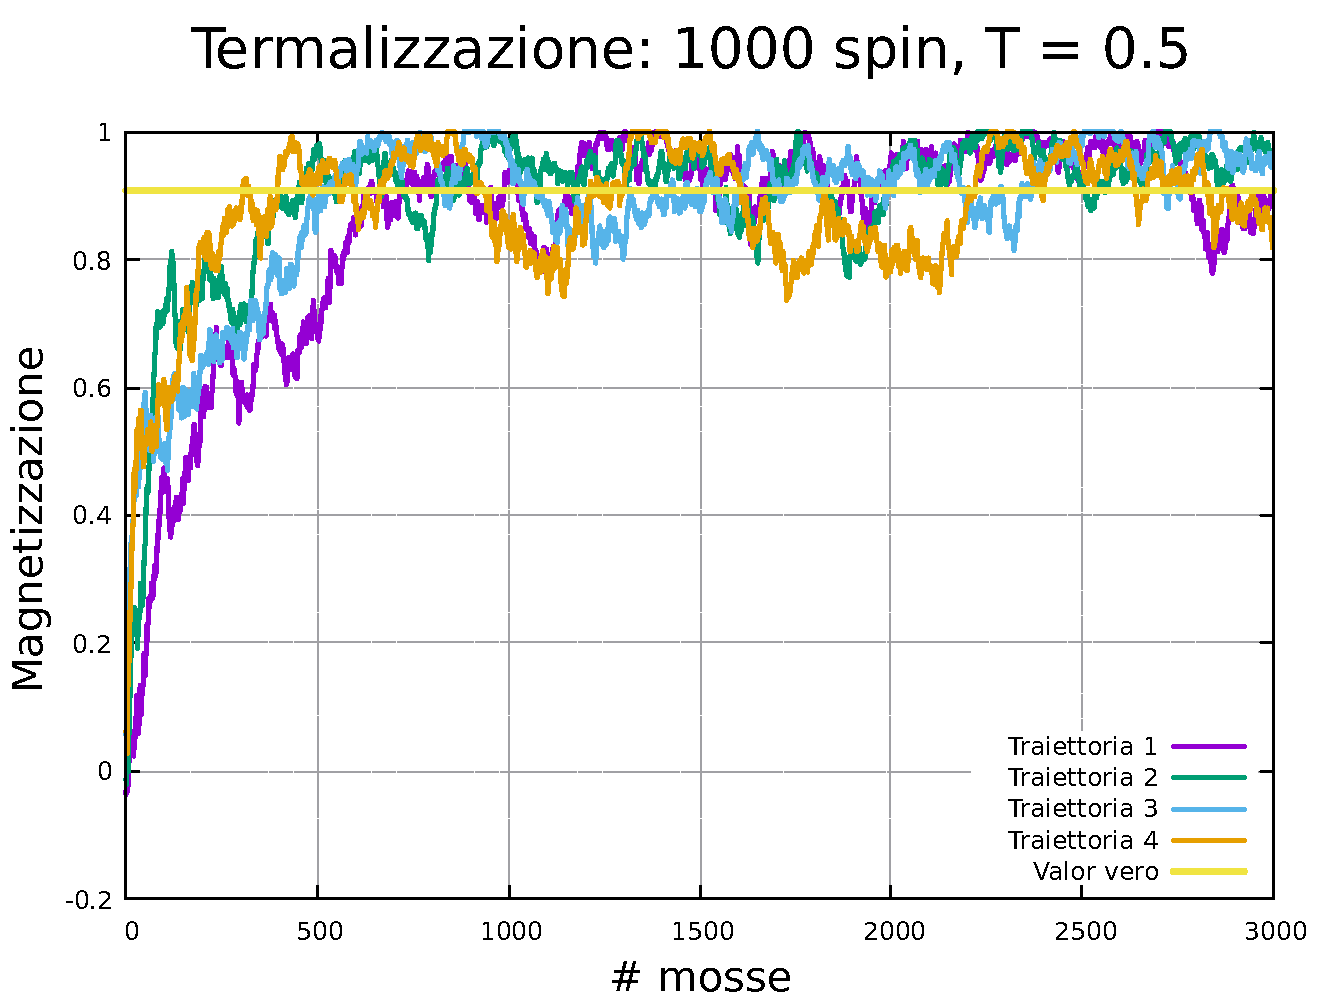
\includegraphics[page=1, width=\textwidth]{Immagini/simIsing1D/magn0.02/term/term_1000_0.5.pdf}
      \caption{$T\,=\,0.5$}
    \end{minipage}\hfill
    \begin{minipage}{0.45\textwidth}  
      \centering
      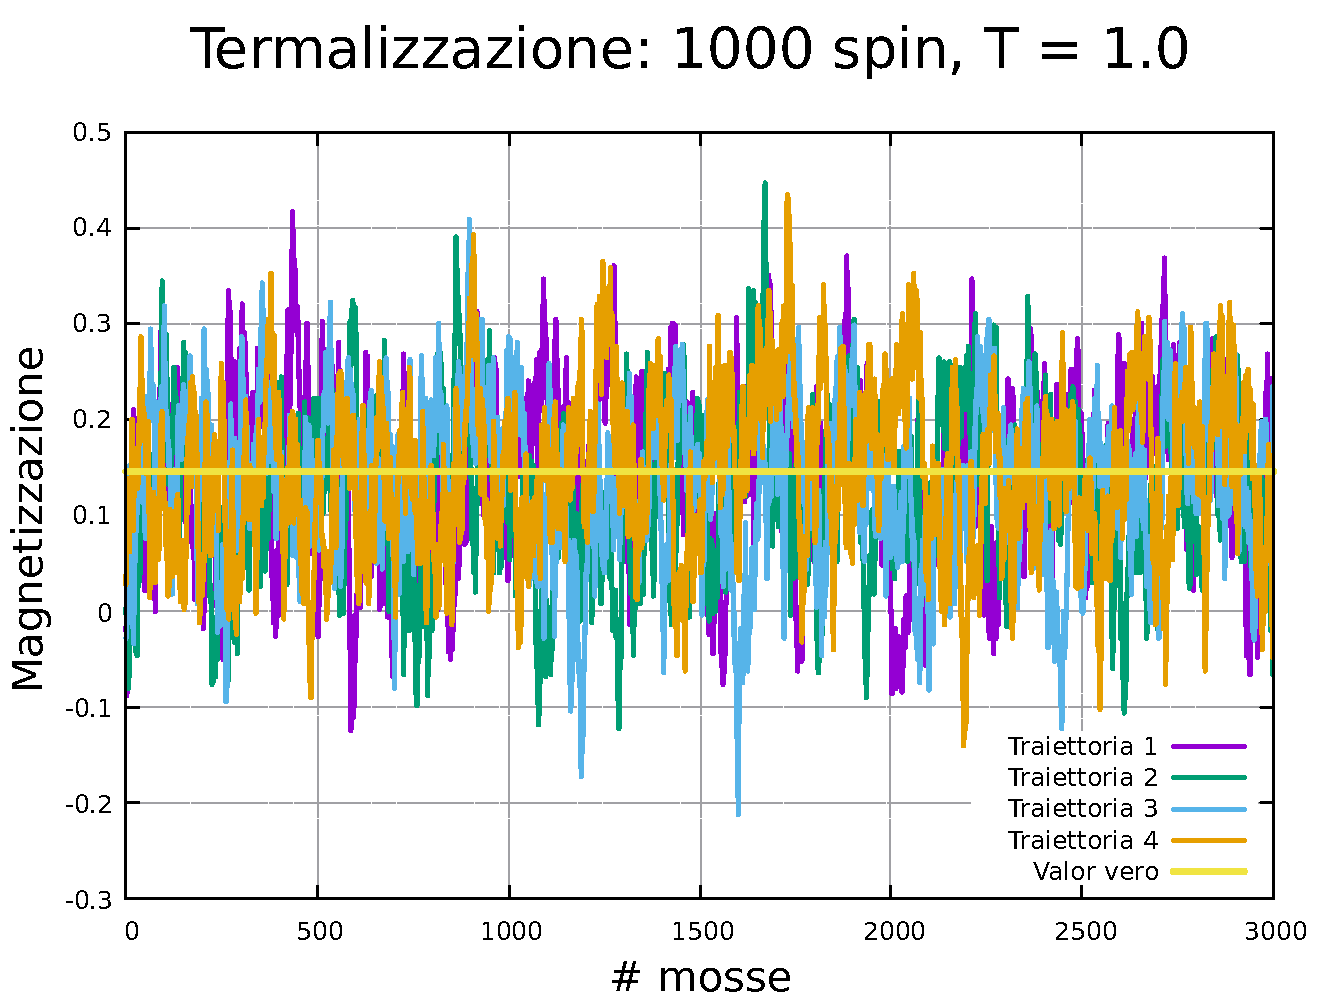
\includegraphics[page=1, width=\textwidth]{Immagini/simIsing1D/magn0.02/term/term_1000_1.0.pdf}
      \caption{$T\,=\,1.0$}
    \end{minipage}
    \vskip\baselineskip 
  
    \begin{minipage}{0.45\textwidth}  
      \centering
      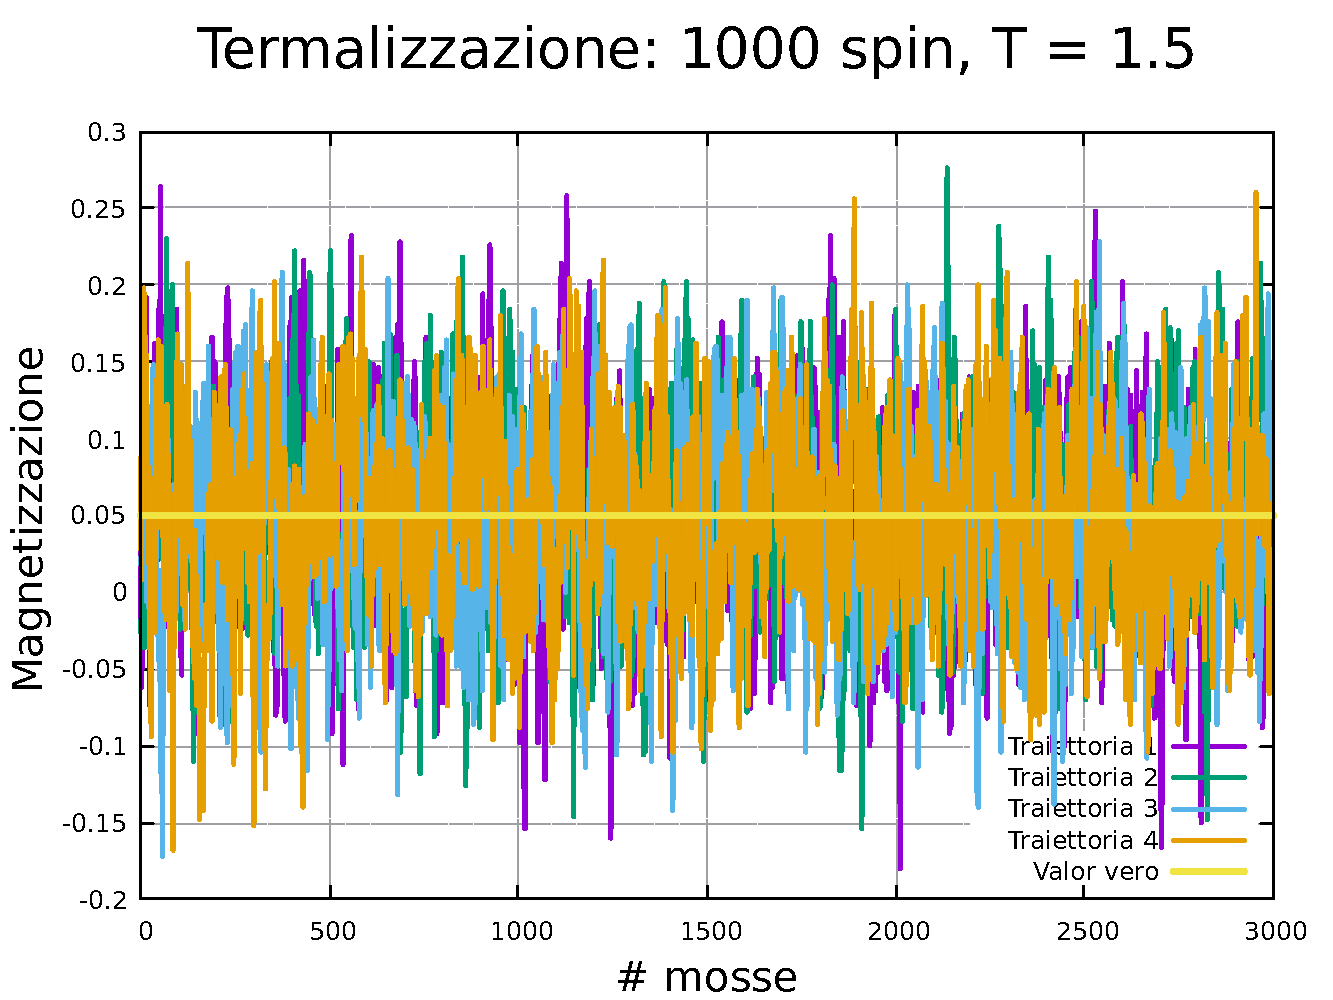
\includegraphics[page=1, width=\textwidth]{Immagini/simIsing1D/magn0.02/term/term_1000_1.5.pdf}
      \caption{$T\,=\,1.5$}
    \end{minipage}\hfill
    \begin{minipage}{0.45\textwidth}  
      \centering
      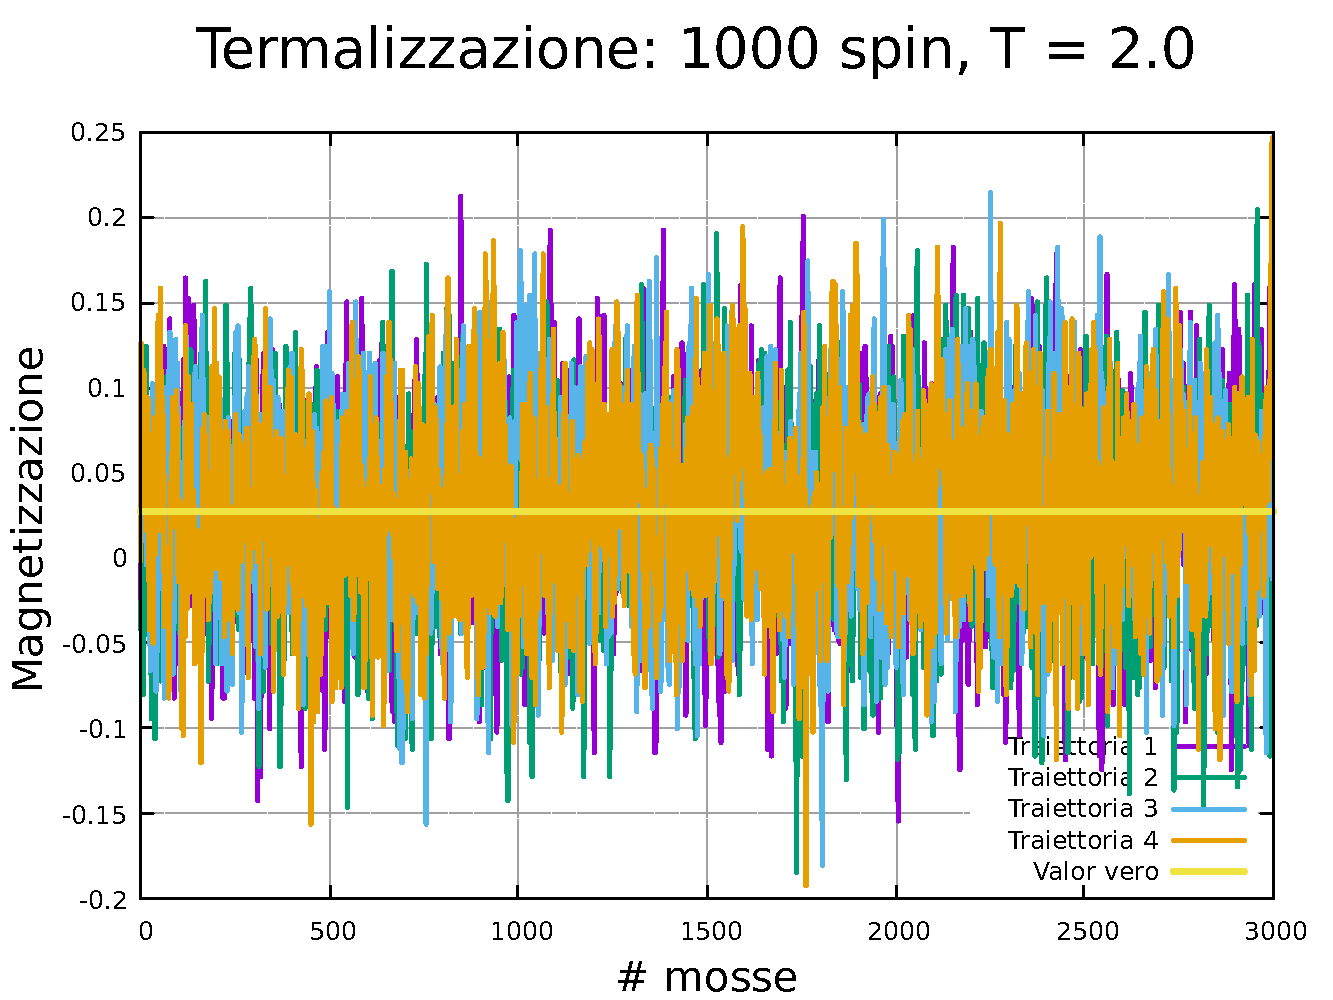
\includegraphics[page=1, width=\textwidth]{Immagini/simIsing1D/magn0.02/term/term_1000_2.0.pdf}
      \caption{$T\,=\,2.0$}
    \end{minipage}
    \caption{Studio della termalizzazione di un modello di Ising 1D: $N_s$ = 1000, h = 0.02.}
\end{figure}

\vspace*{\fill}

\newpage

\vspace*{\fill}

\begin{figure}[htbp]
    \centering
    \begin{minipage}{0.45\textwidth}  
      \centering
      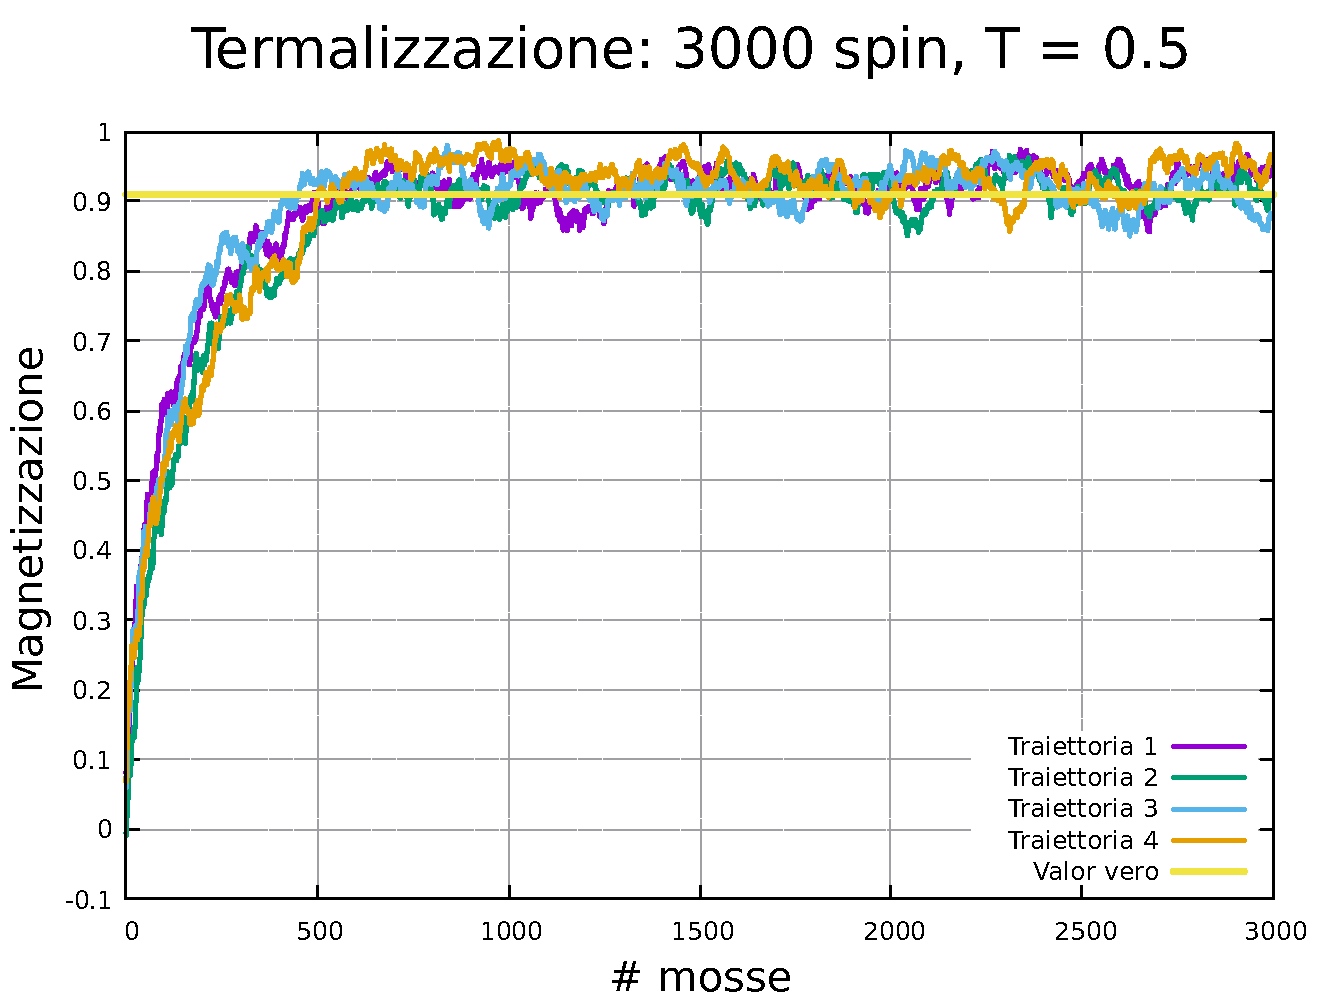
\includegraphics[page=1, width=\textwidth]{Immagini/simIsing1D/magn0.02/term/term_3000_0.5.pdf}
      \caption{$T\,=\,0.5$}
    \end{minipage}\hfill
    \begin{minipage}{0.45\textwidth}  
      \centering
      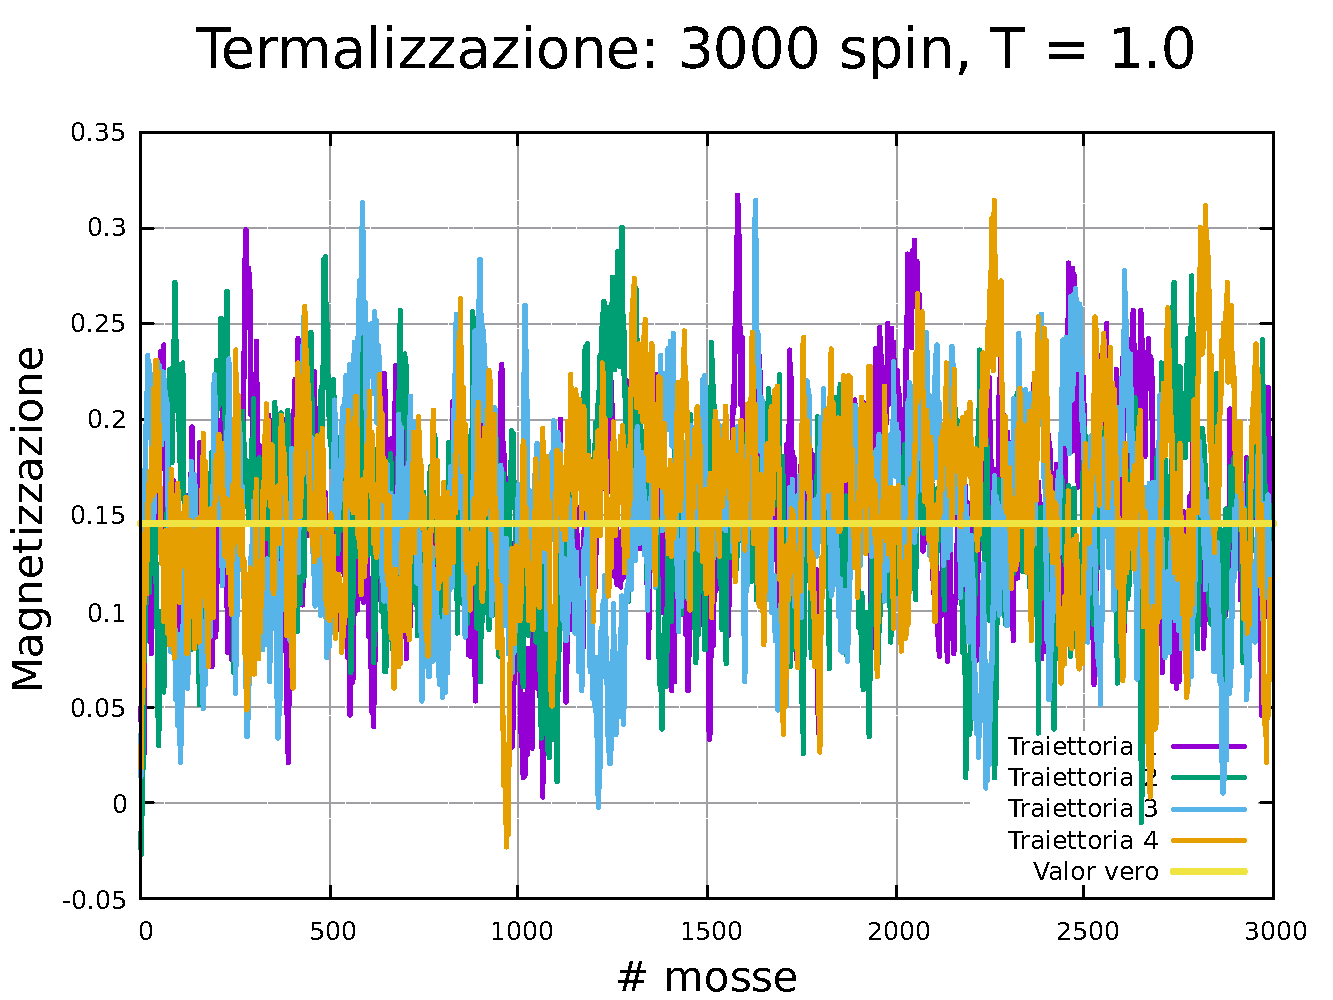
\includegraphics[page=1, width=\textwidth]{Immagini/simIsing1D/magn0.02/term/term_3000_1.0.pdf}
      \caption{$T\,=\,1.0$}
    \end{minipage}
    \vskip\baselineskip 
  
    \begin{minipage}{0.45\textwidth}  
      \centering
      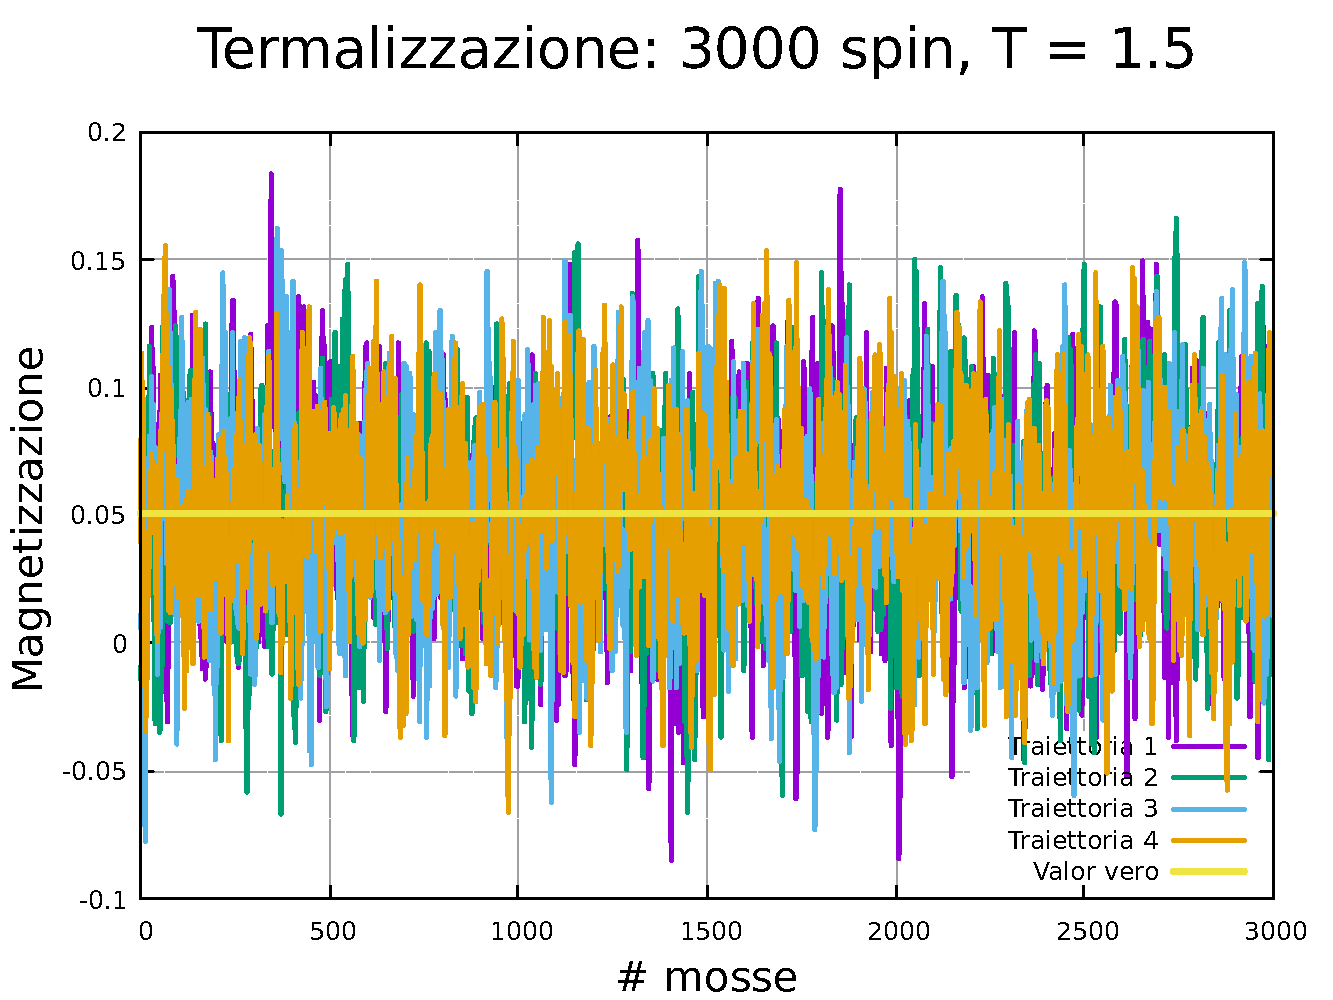
\includegraphics[page=1, width=\textwidth]{Immagini/simIsing1D/magn0.02/term/term_3000_1.5.pdf}
      \caption{$T\,=\,1.5$}
    \end{minipage}\hfill
    \begin{minipage}{0.45\textwidth}  
      \centering
      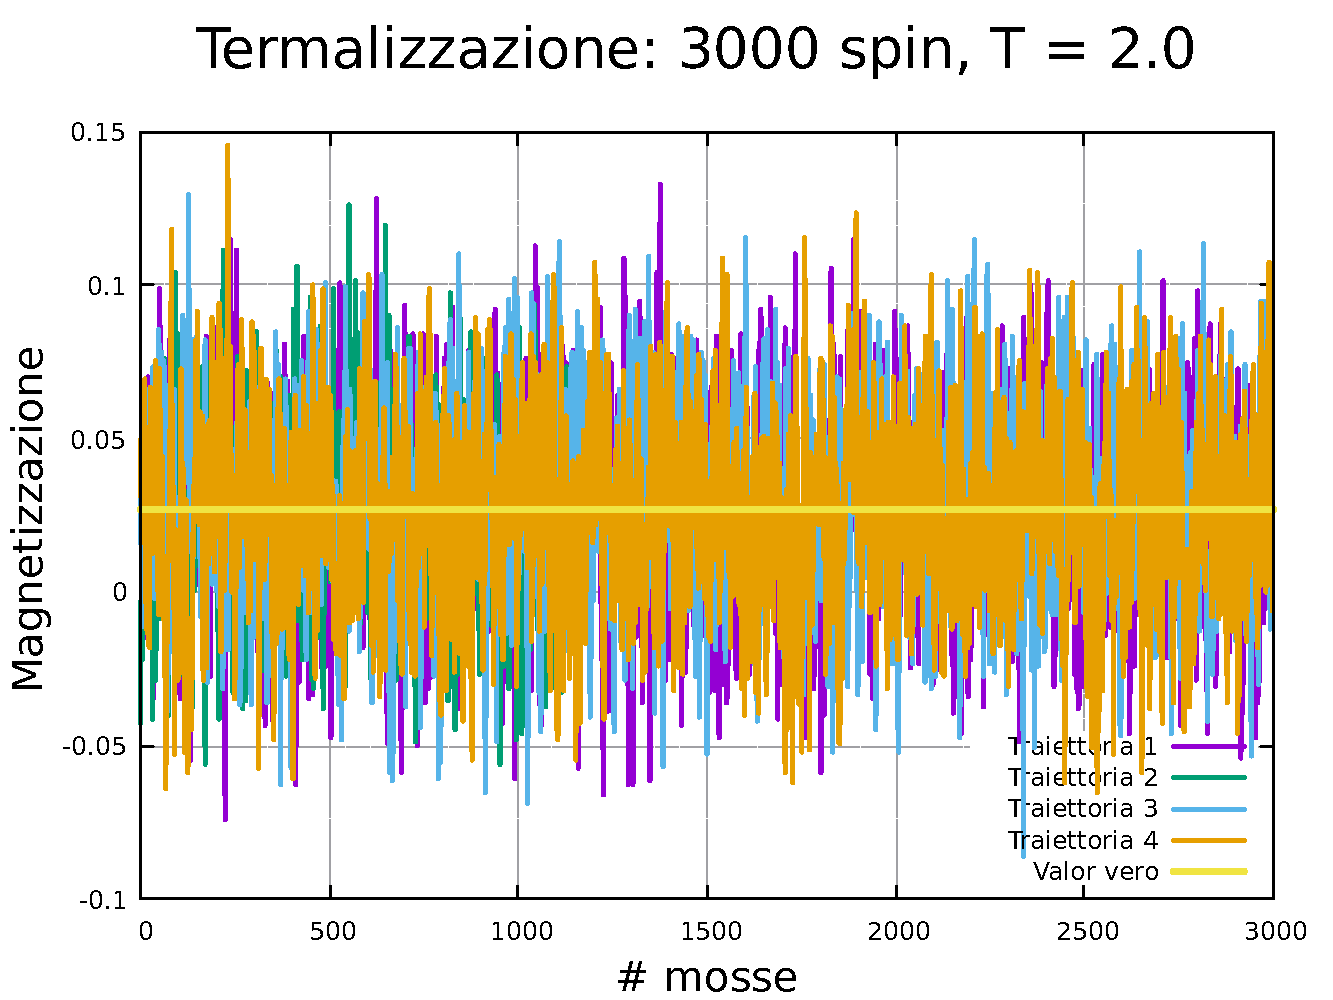
\includegraphics[page=1, width=\textwidth]{Immagini/simIsing1D/magn0.02/term/term_3000_2.0.pdf}
      \caption{$T\,=\,2.0$}
    \end{minipage}
    \caption{Studio della termalizzazione di un modello di Ising 1D: $N_s$ = 3000, h = 0.02.}
\end{figure}

\vspace*{\fill}

\newpage

\vspace*{\fill}

\begin{figure}[htbp]
    \centering
    \begin{minipage}{0.45\textwidth}  
      \centering
      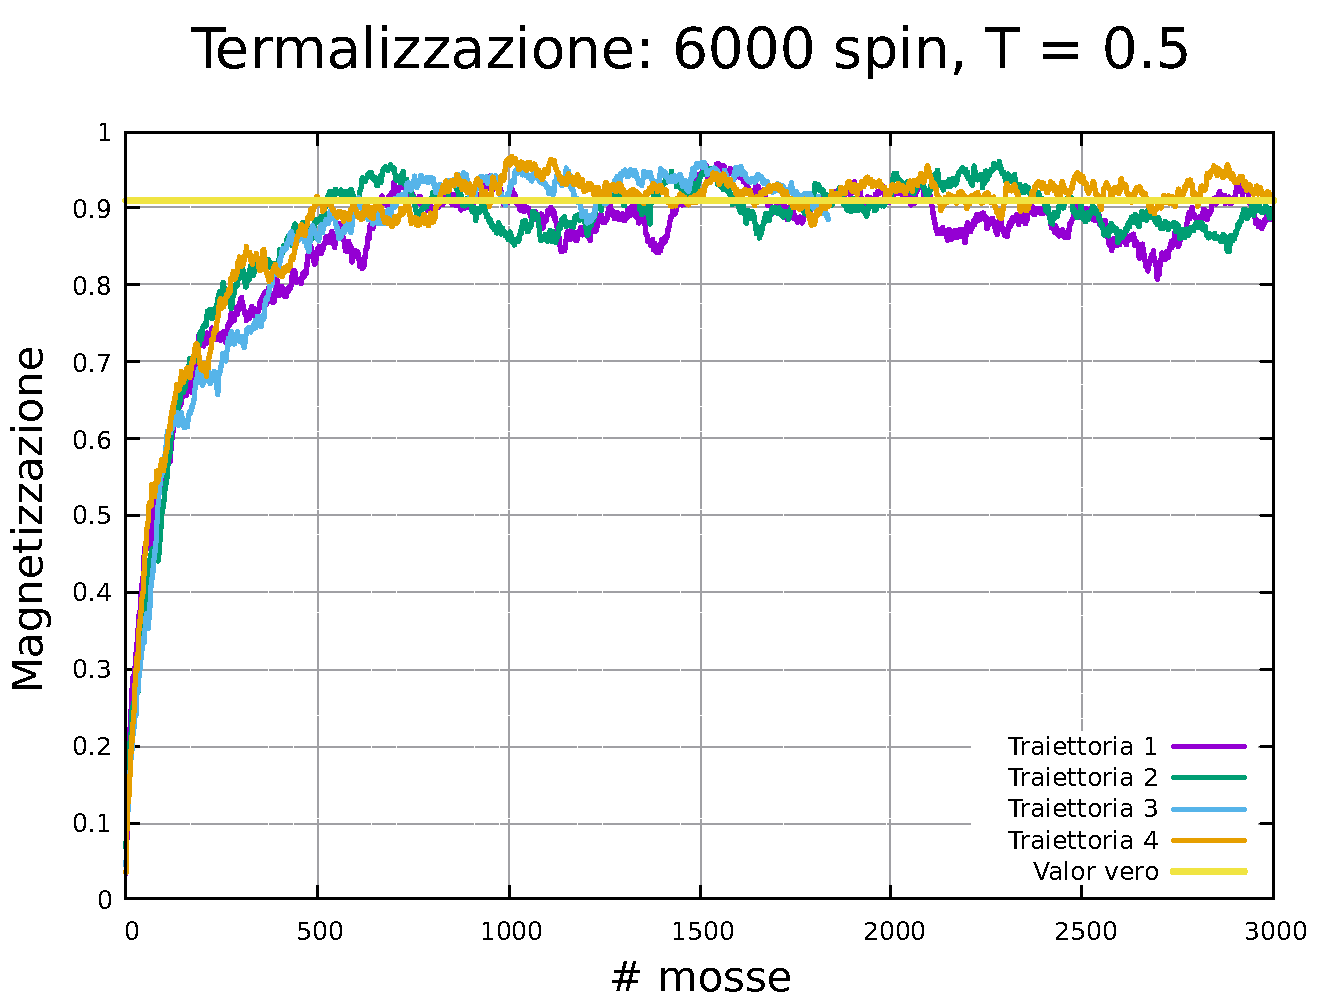
\includegraphics[page=1, width=\textwidth]{Immagini/simIsing1D/magn0.02/term/term_6000_0.5.pdf}
      \caption{$T\,=\,0.5$}
    \end{minipage}\hfill
    \begin{minipage}{0.45\textwidth}  
      \centering
      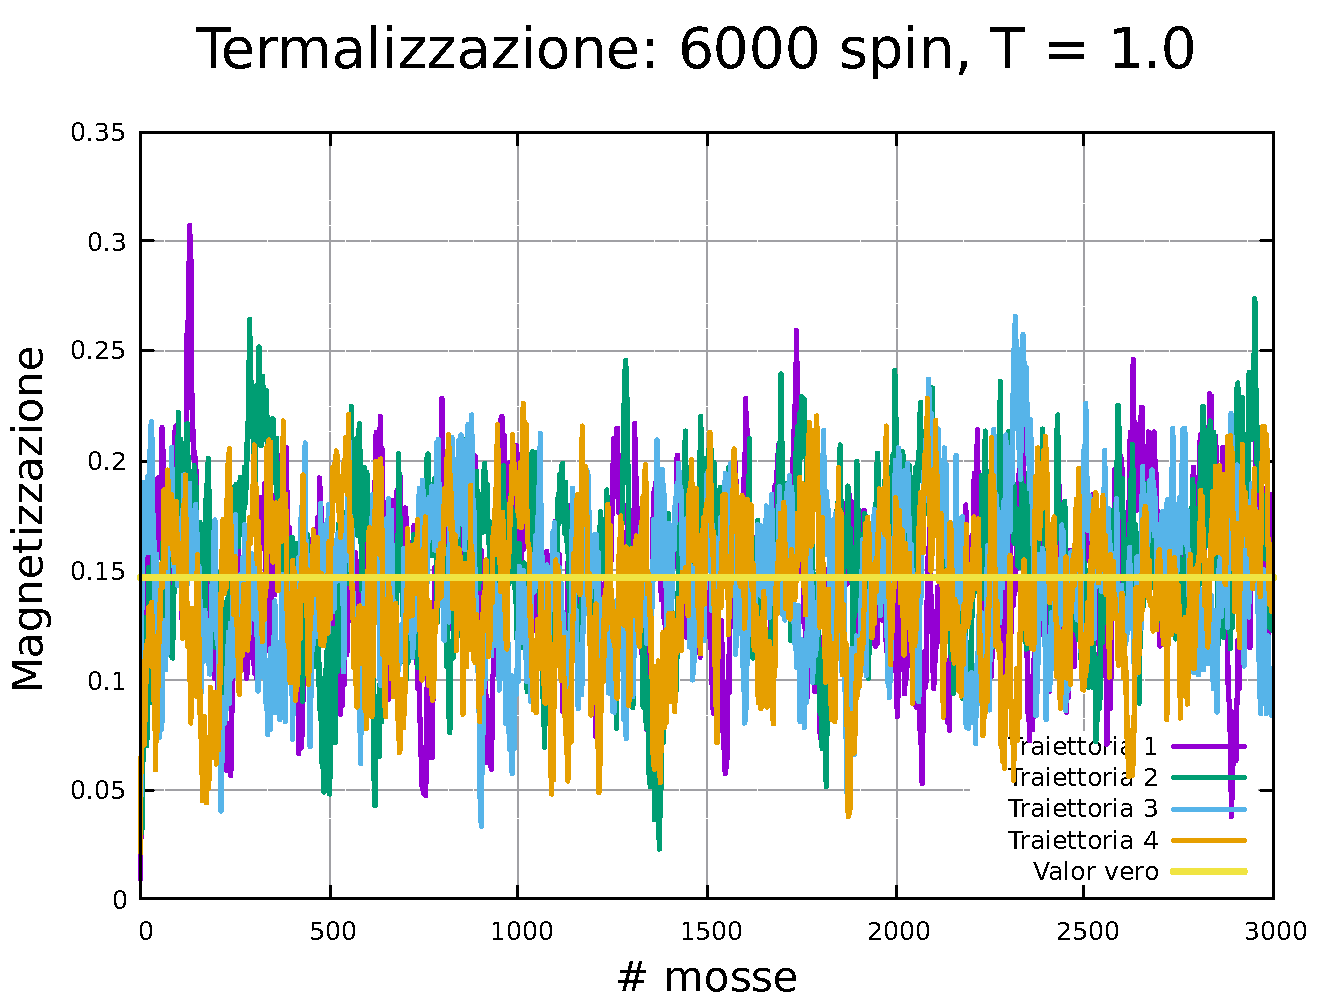
\includegraphics[page=1, width=\textwidth]{Immagini/simIsing1D/magn0.02/term/term_6000_1.0.pdf}
      \caption{$T\,=\,1.0$}
    \end{minipage}
    \vskip\baselineskip 
  
    \begin{minipage}{0.45\textwidth}  
      \centering
      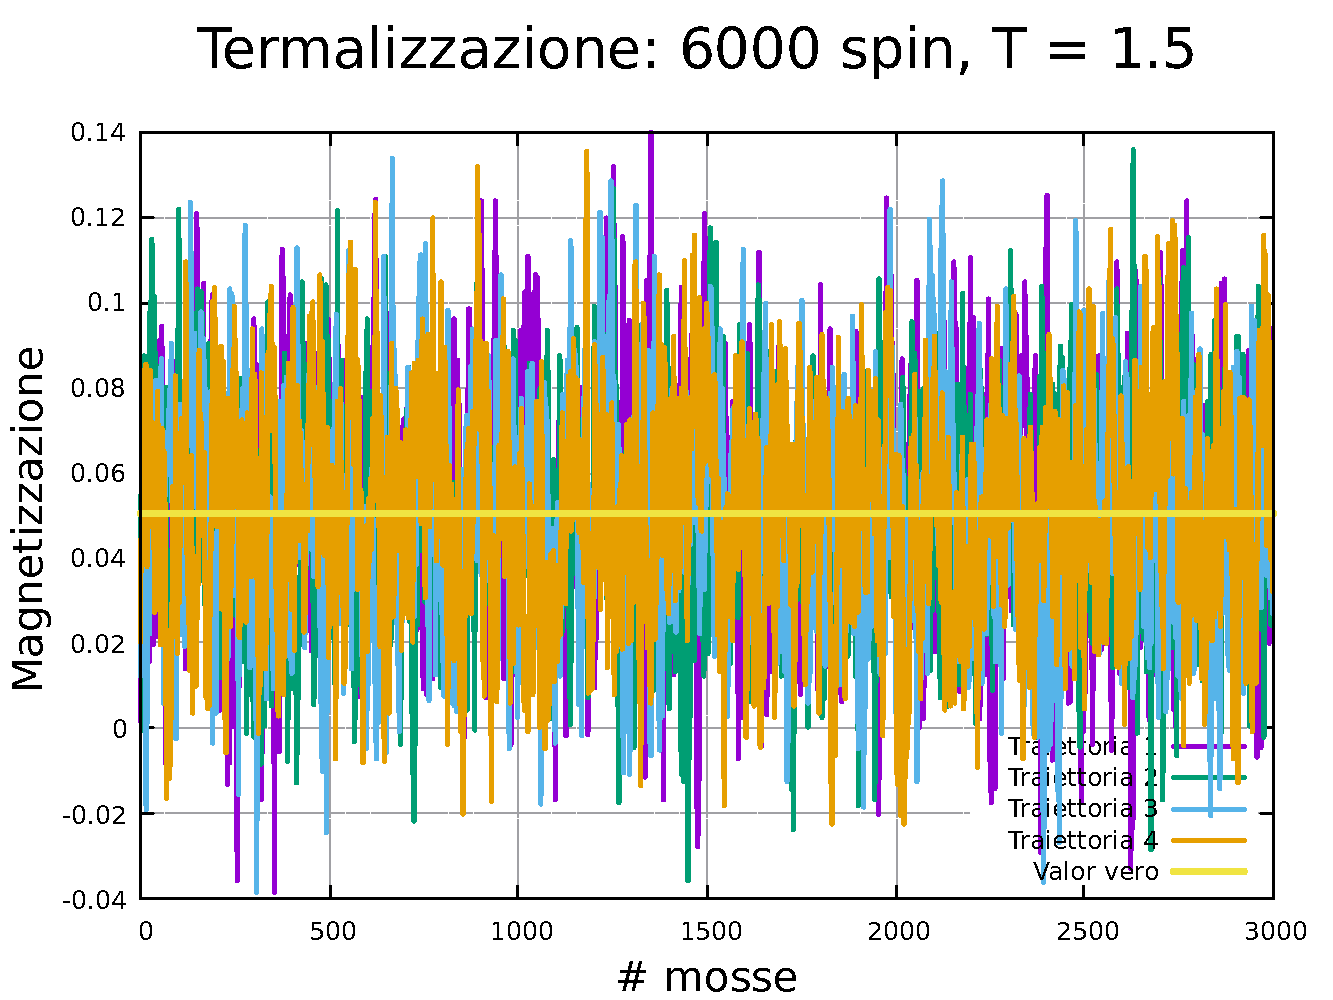
\includegraphics[page=1, width=\textwidth]{Immagini/simIsing1D/magn0.02/term/term_6000_1.5.pdf}
      \caption{$T\,=\,1.5$}
    \end{minipage}\hfill
    \begin{minipage}{0.45\textwidth}  
      \centering
      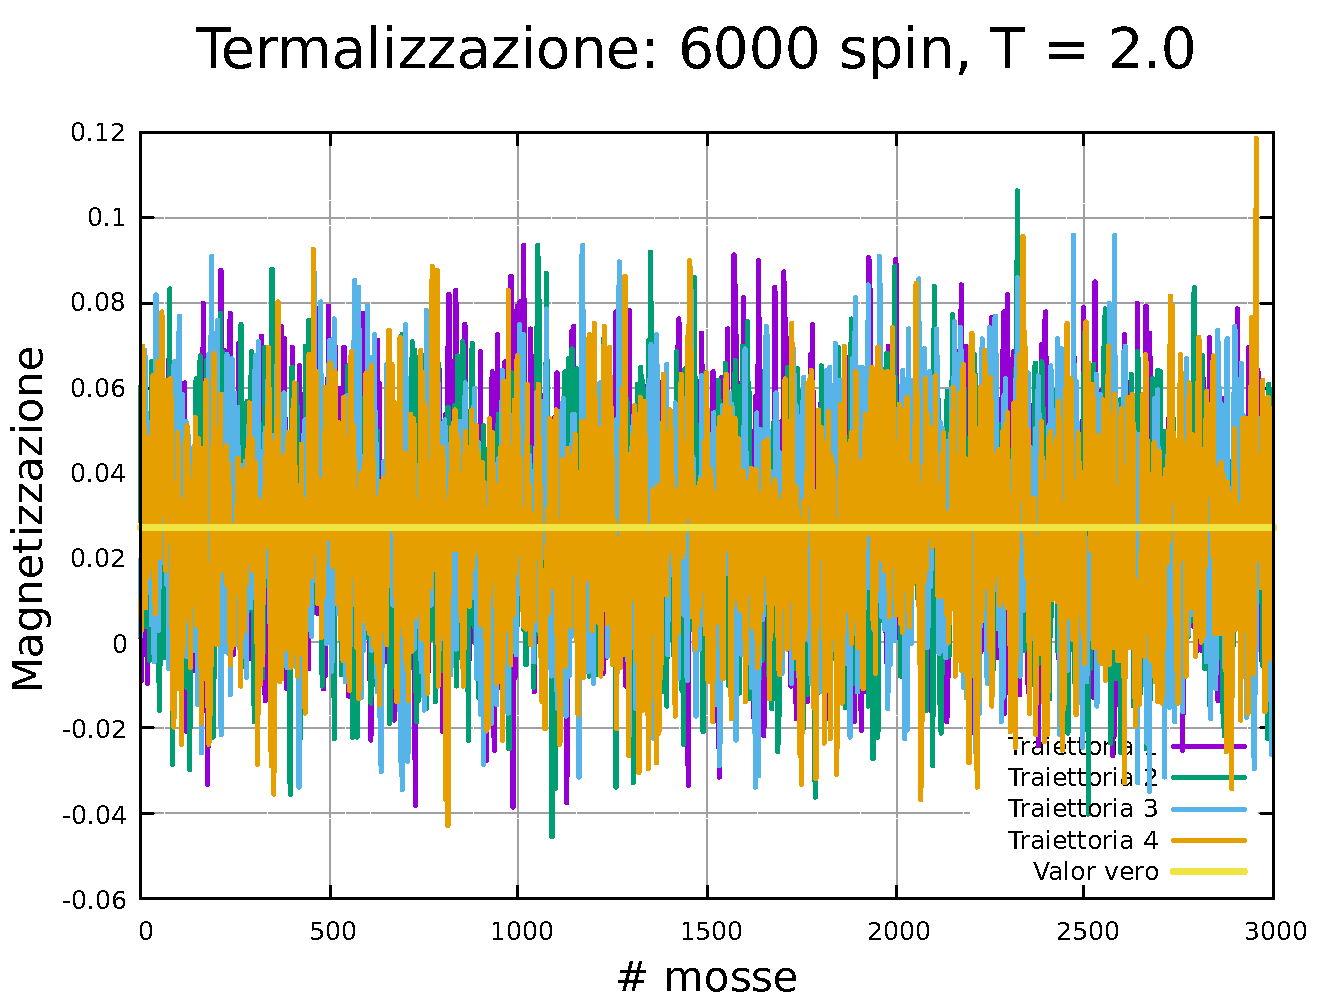
\includegraphics[page=1, width=\textwidth]{Immagini/simIsing1D/magn0.02/term/term_6000_2.0.pdf}
      \caption{$T\,=\,2.0$}
    \end{minipage}
    \caption{Studio della termalizzazione di un modello di Ising 1D: $N_s$ = 6000, h = 0.02.}
\end{figure}

\vspace*{\fill}

\newpage

\vspace*{\fill}

\begin{figure}[htbp]
    \centering
    \begin{minipage}{0.45\textwidth}  
      \centering
      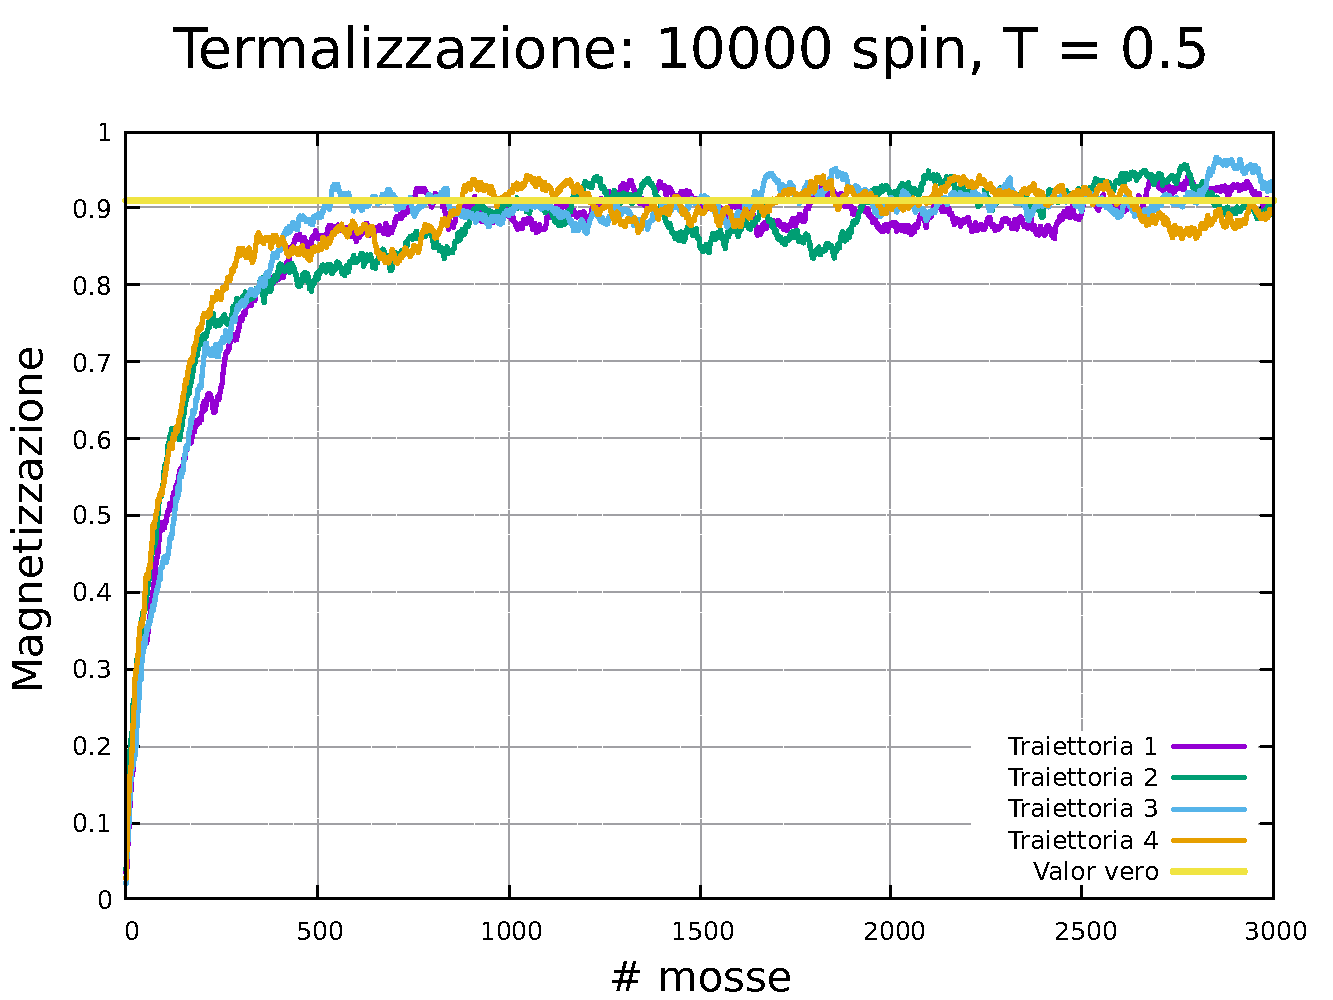
\includegraphics[page=1, width=\textwidth]{Immagini/simIsing1D/magn0.02/term/term_10000_0.5.pdf}
      \caption{$T\,=\,0.5$}
    \end{minipage}\hfill
    \begin{minipage}{0.45\textwidth}  
      \centering
      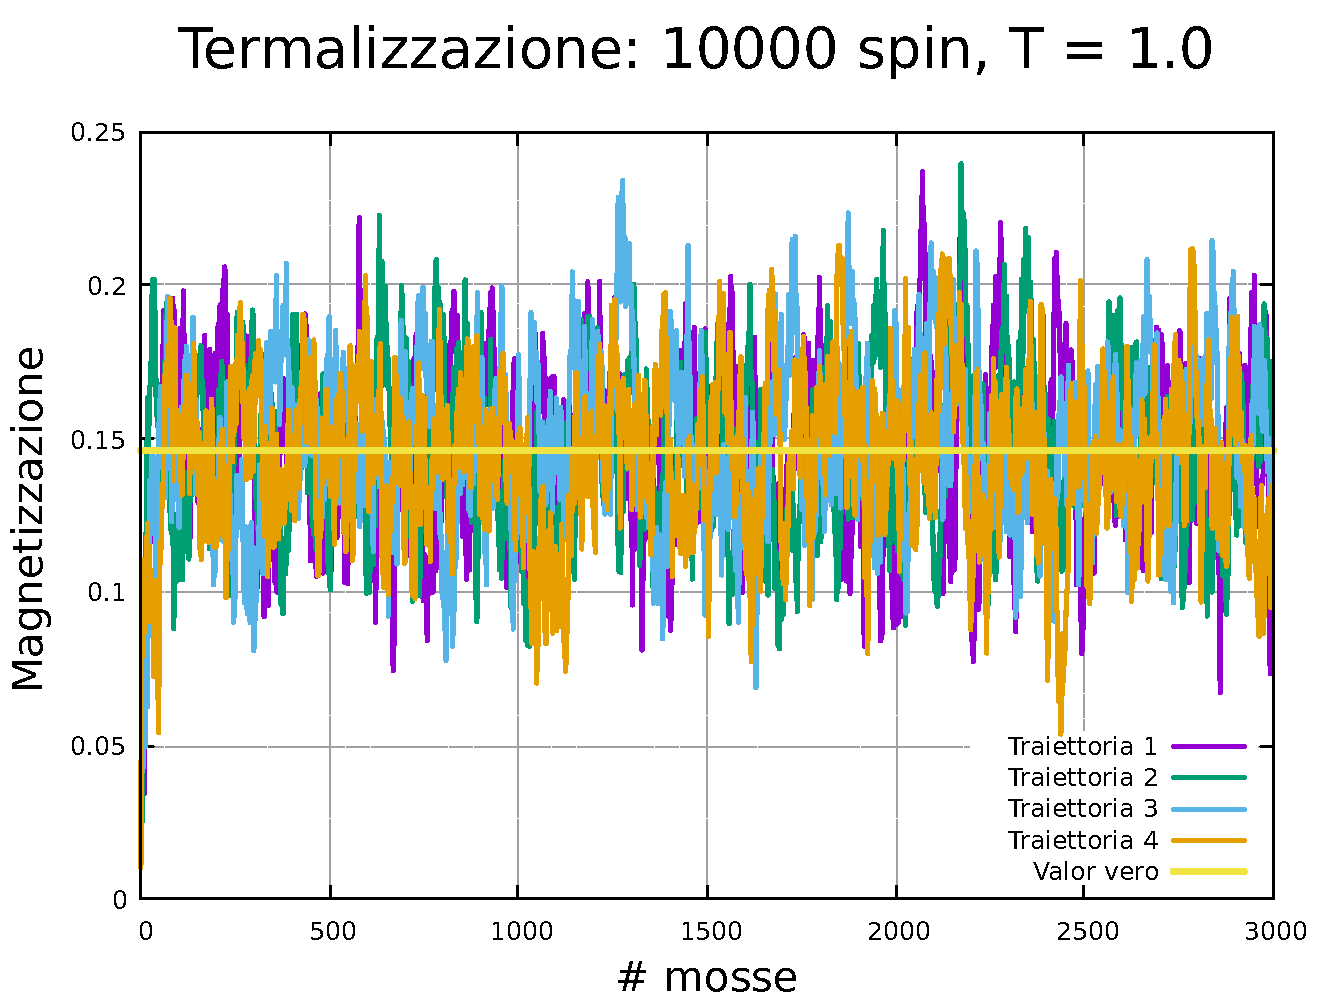
\includegraphics[page=1, width=\textwidth]{Immagini/simIsing1D/magn0.02/term/term_10000_1.0.pdf}
      \caption{$T\,=\,1.0$}
    \end{minipage}
    \vskip\baselineskip 
  
    \begin{minipage}{0.45\textwidth}  
      \centering
      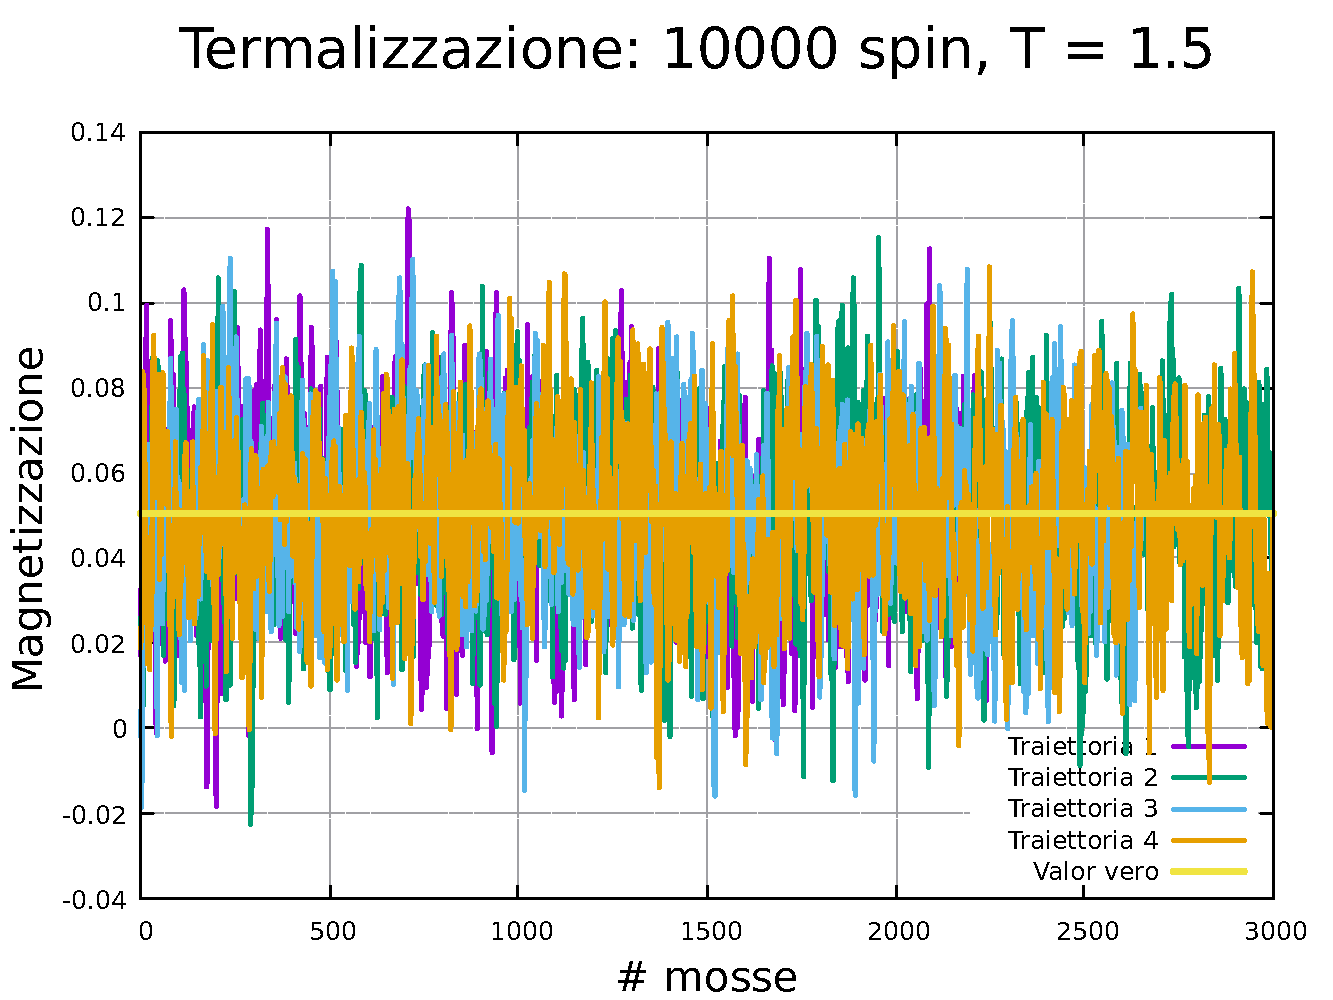
\includegraphics[page=1, width=\textwidth]{Immagini/simIsing1D/magn0.02/term/term_10000_1.5.pdf}
      \caption{$T\,=\,1.5$}
    \end{minipage}\hfill
    \begin{minipage}{0.45\textwidth}  
      \centering
      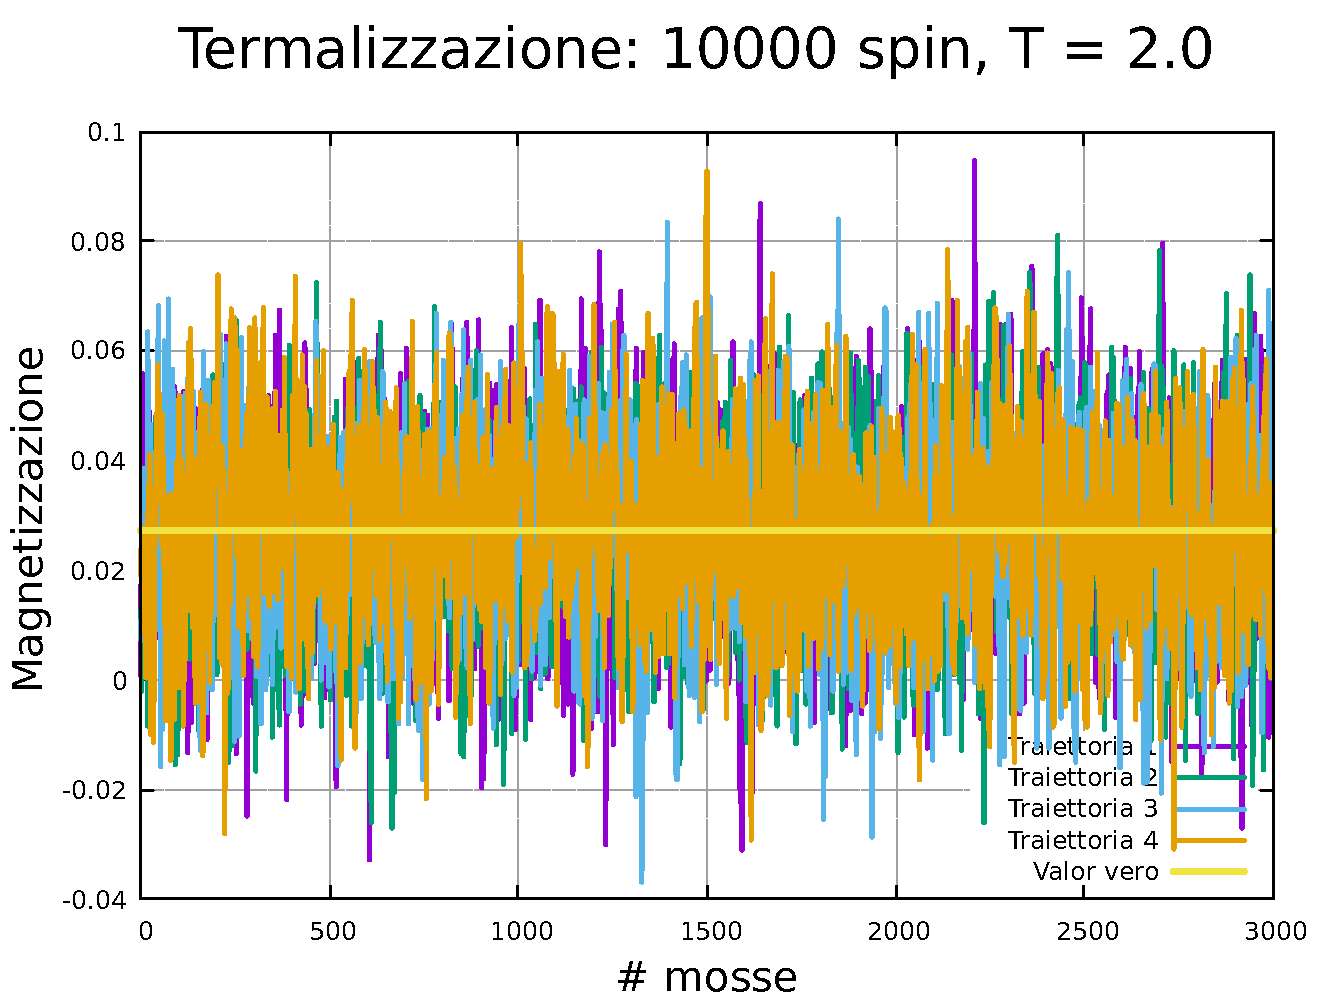
\includegraphics[page=1, width=\textwidth]{Immagini/simIsing1D/magn0.02/term/term_10000_2.0.pdf}
      \caption{$T\,=\,2.0$}
    \end{minipage}
    \caption{Studio della termalizzazione di un modello di Ising 1D: $N_s$ = 10000, h = 0.02.}
\end{figure}

\vspace*{\fill}

\newpage



\subsection{Auto-correlazione}

\vspace*{\fill}

\begin{figure}[htbp]
    \centering
    \begin{minipage}{0.45\textwidth}  
      \centering
      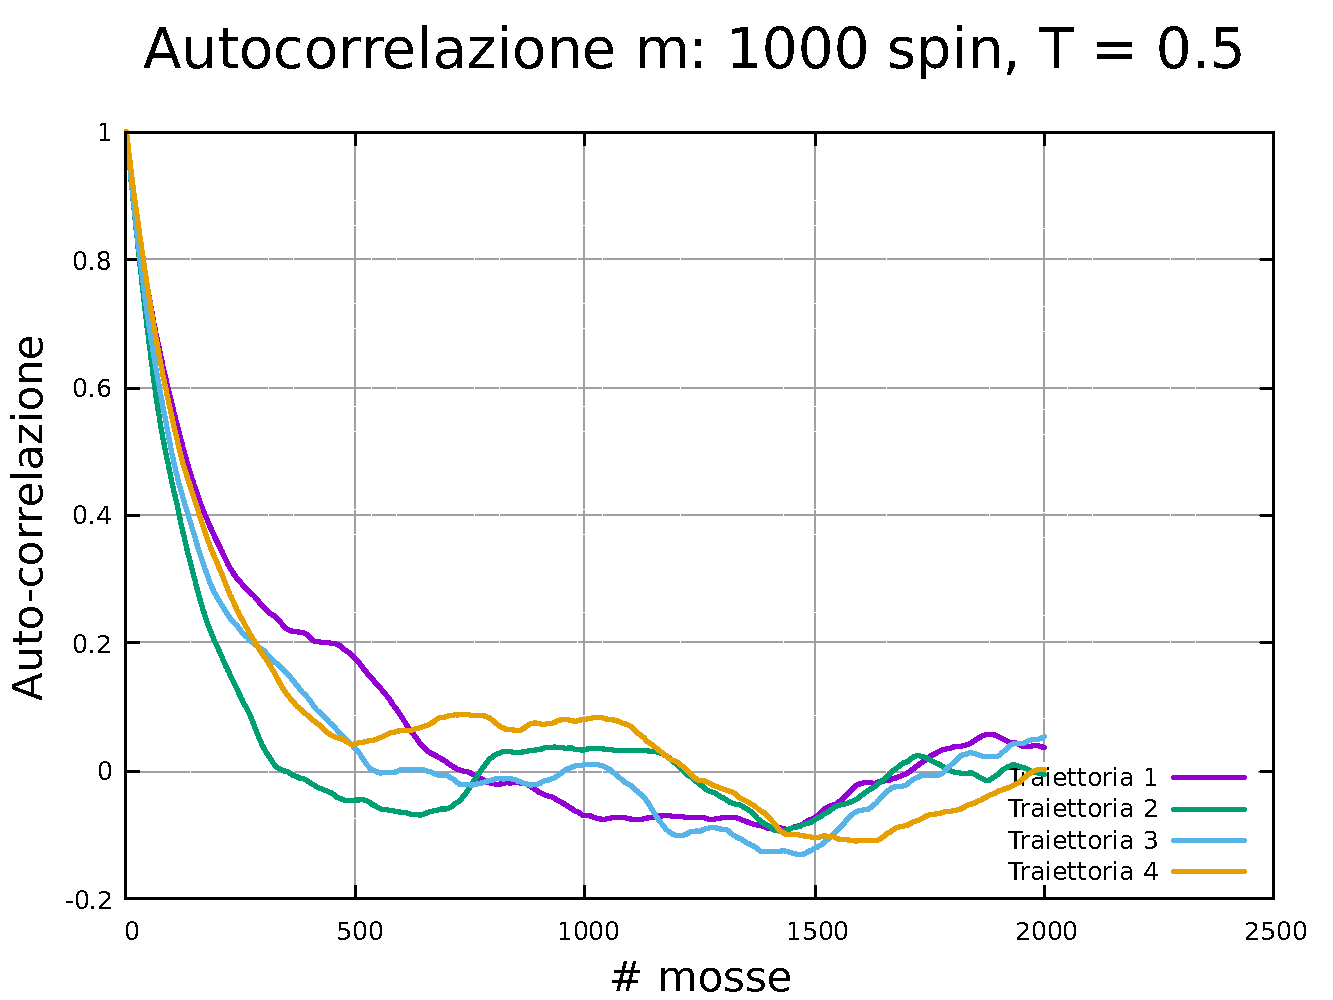
\includegraphics[page=1, width=\textwidth]{Immagini/simIsing1D/magn0.02/tcorr/tcorr_1000_0.5.pdf}
      \caption{$T\,=\,0.5$}
    \end{minipage}\hfill
    \begin{minipage}{0.45\textwidth}  
      \centering
      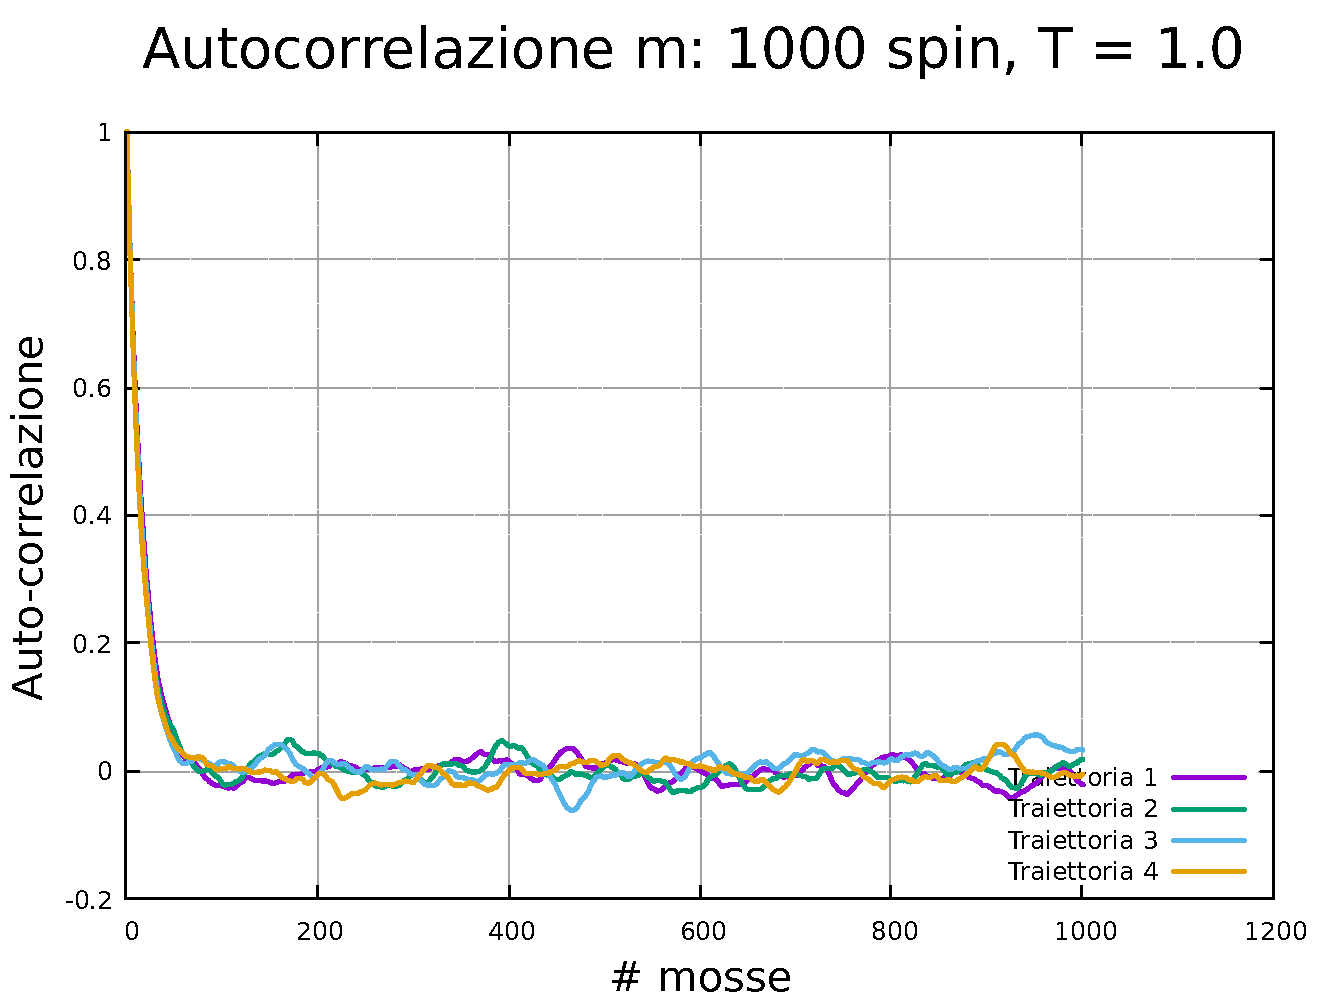
\includegraphics[page=1, width=\textwidth]{Immagini/simIsing1D/magn0.02/tcorr/tcorr_1000_1.0.pdf}
      \caption{$T\,=\,1.0$}
    \end{minipage}
    \vskip\baselineskip 
  
    \begin{minipage}{0.45\textwidth}  
      \centering
      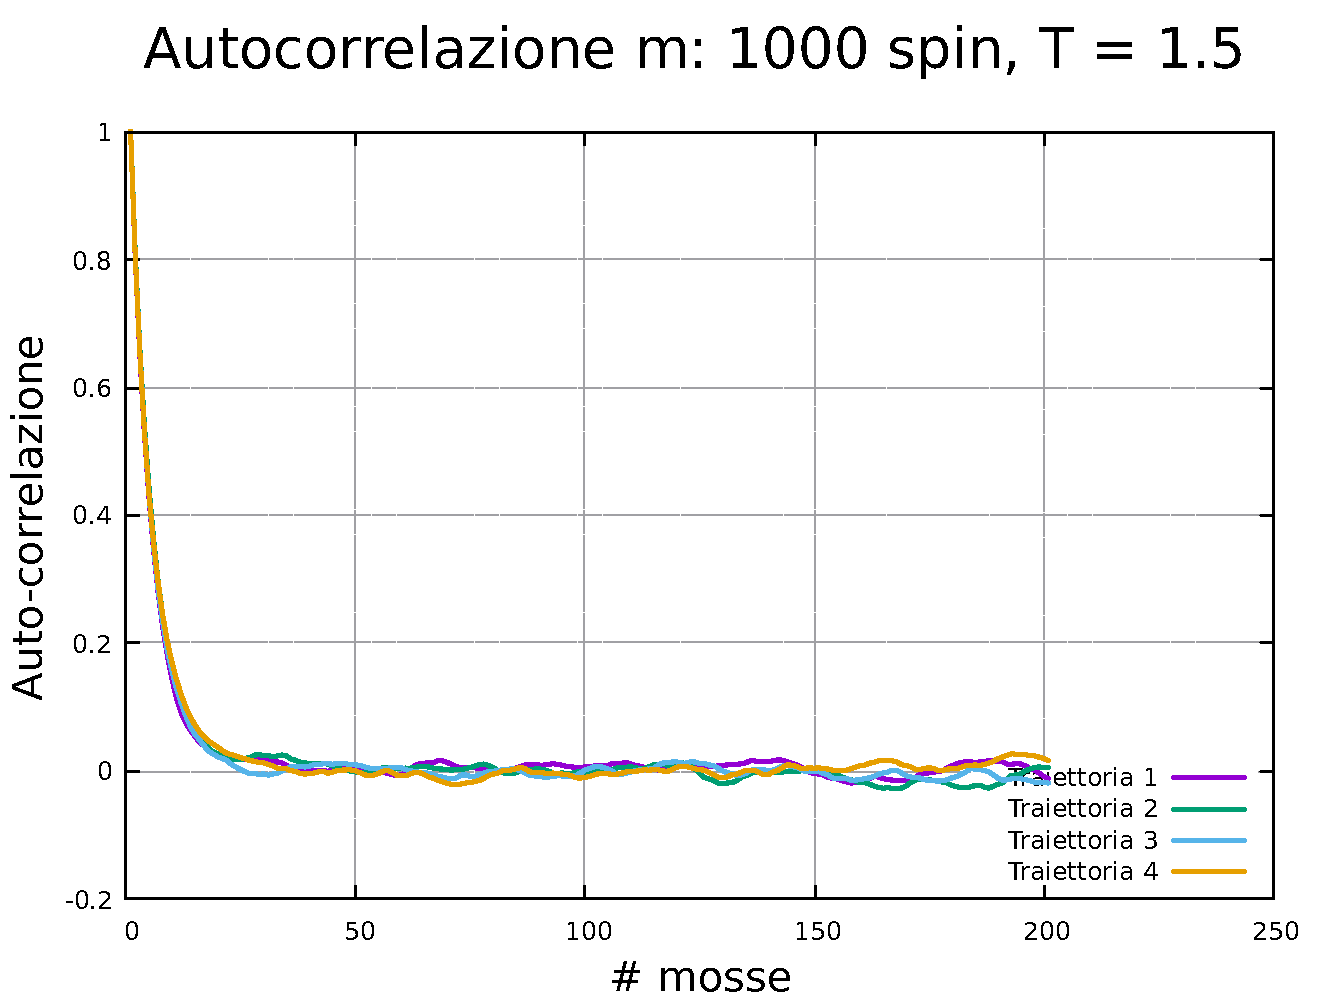
\includegraphics[page=1, width=\textwidth]{Immagini/simIsing1D/magn0.02/tcorr/tcorr_1000_1.5.pdf}
      \caption{$T\,=\,1.5$}
    \end{minipage}\hfill
    \begin{minipage}{0.45\textwidth}  
      \centering
      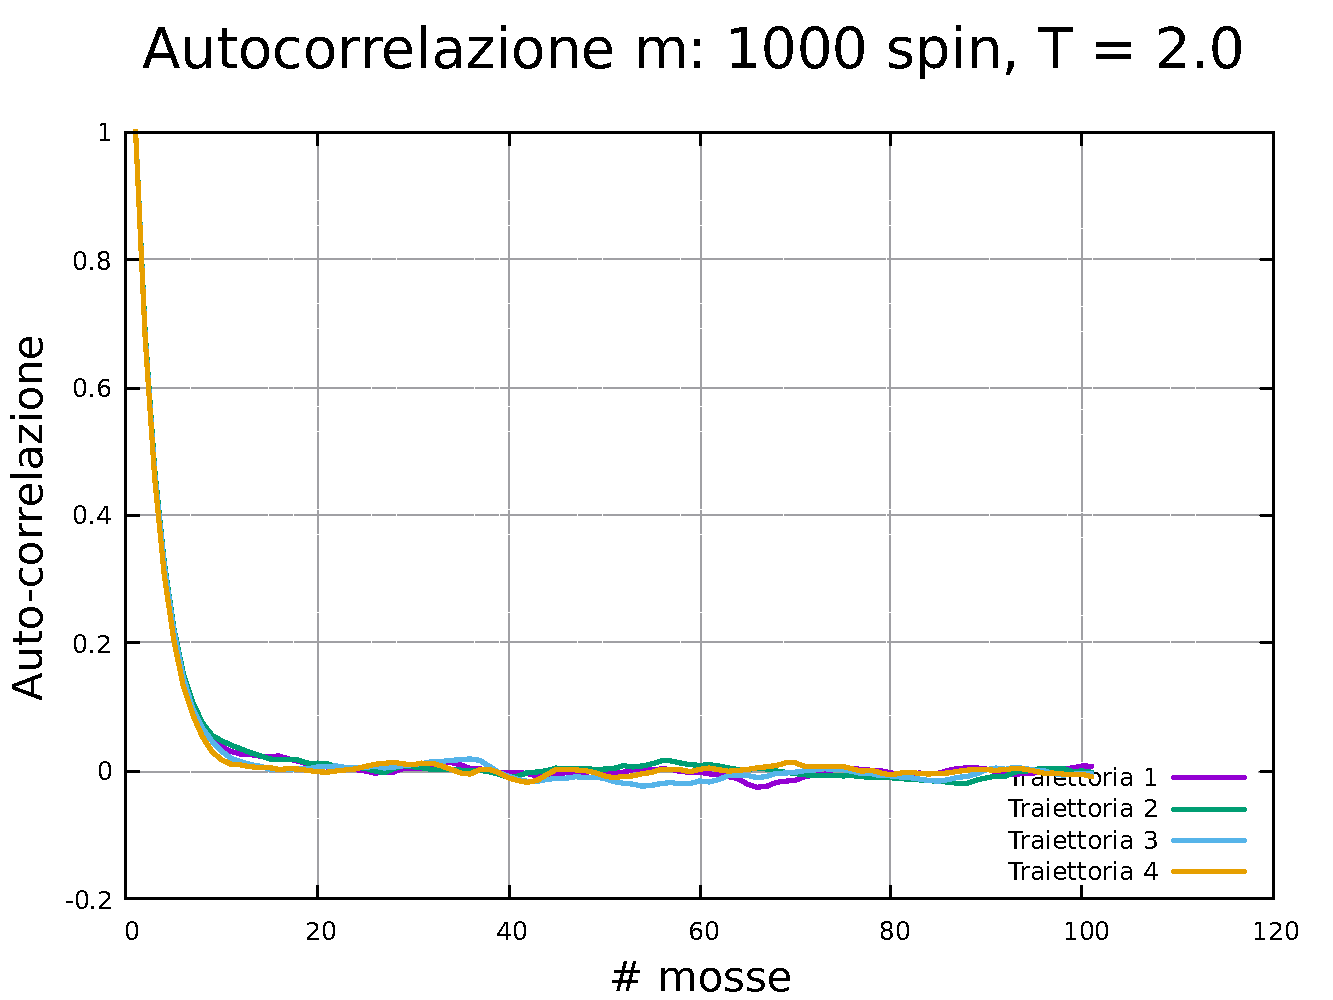
\includegraphics[page=1, width=\textwidth]{Immagini/simIsing1D/magn0.02/tcorr/tcorr_1000_2.0.pdf}
      \caption{$T\,=\,2.0$}
    \end{minipage}
    \caption{Studio dell'auto-correlazione per un modello di Ising 1D: $N_s$ = 1000, h = 0.02.}
\end{figure}

\vspace*{\fill}

\newpage

\vspace*{\fill}

\begin{figure}[htbp]
    \centering
    \begin{minipage}{0.45\textwidth}  
      \centering
      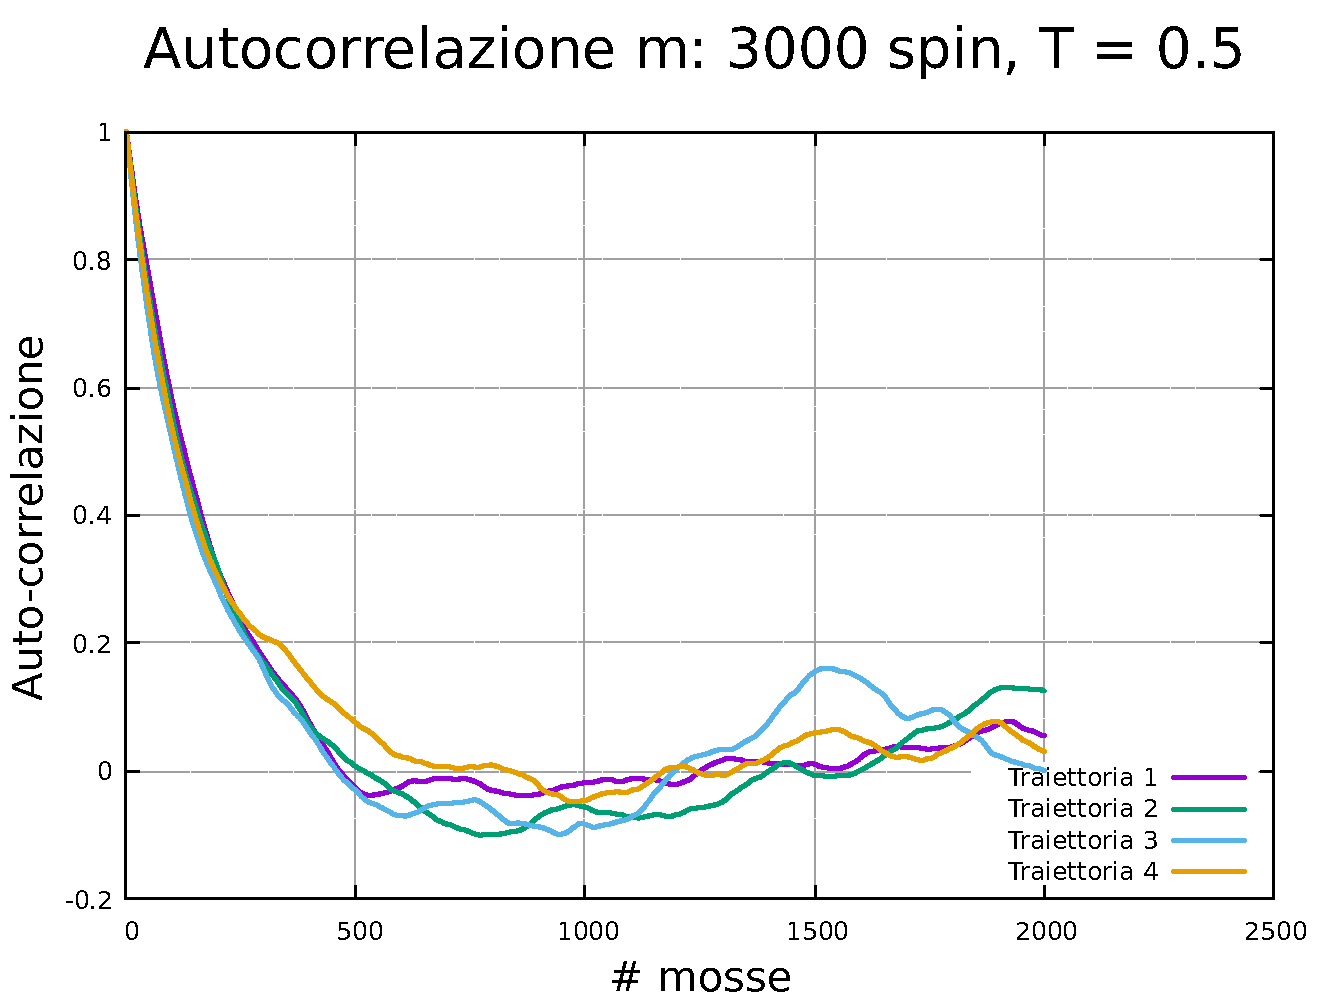
\includegraphics[page=1, width=\textwidth]{Immagini/simIsing1D/magn0.02/tcorr/tcorr_3000_0.5.pdf}
      \caption{$T\,=\,0.5$}
    \end{minipage}\hfill
    \begin{minipage}{0.45\textwidth}  
      \centering
      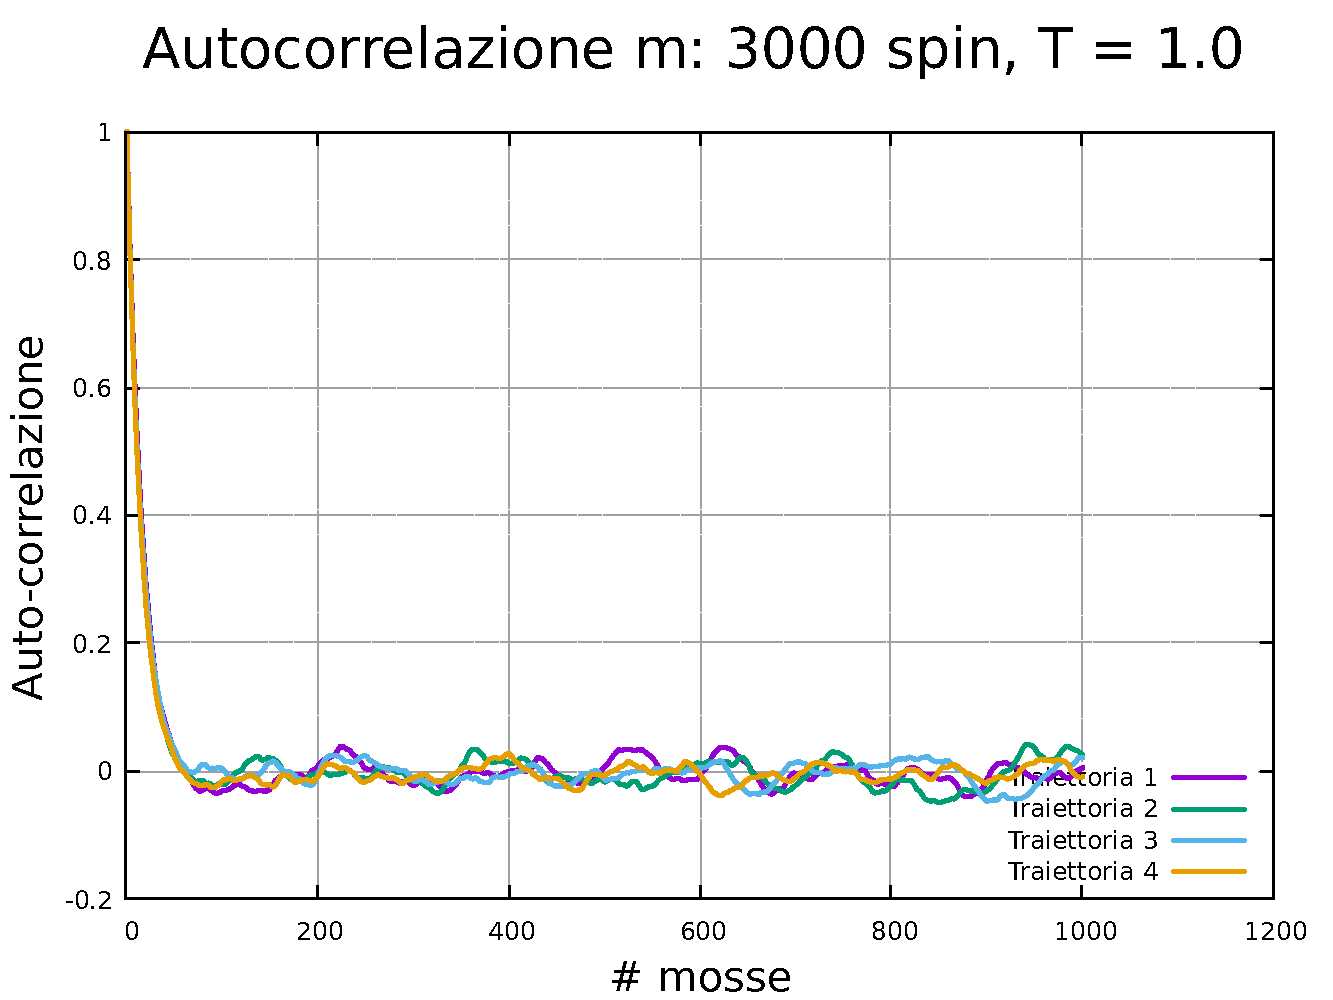
\includegraphics[page=1, width=\textwidth]{Immagini/simIsing1D/magn0.02/tcorr/tcorr_3000_1.0.pdf}
      \caption{$T\,=\,1.0$}
    \end{minipage}
    \vskip\baselineskip 
  
    \begin{minipage}{0.45\textwidth}  
      \centering
      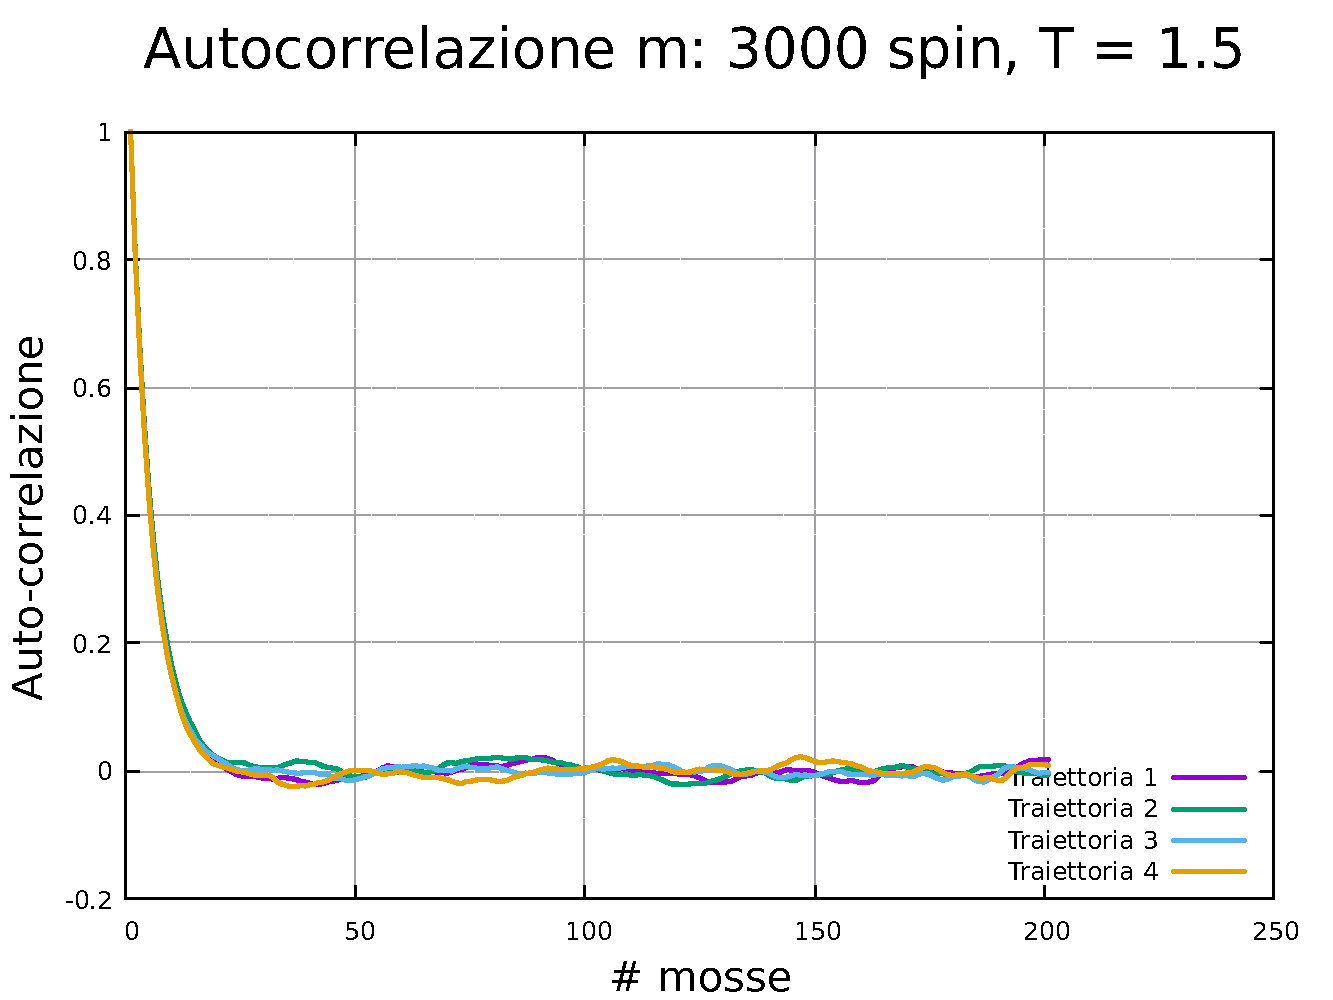
\includegraphics[page=1, width=\textwidth]{Immagini/simIsing1D/magn0.02/tcorr/tcorr_3000_1.5.pdf}
      \caption{$T\,=\,1.5$}
    \end{minipage}\hfill
    \begin{minipage}{0.45\textwidth}  
      \centering
      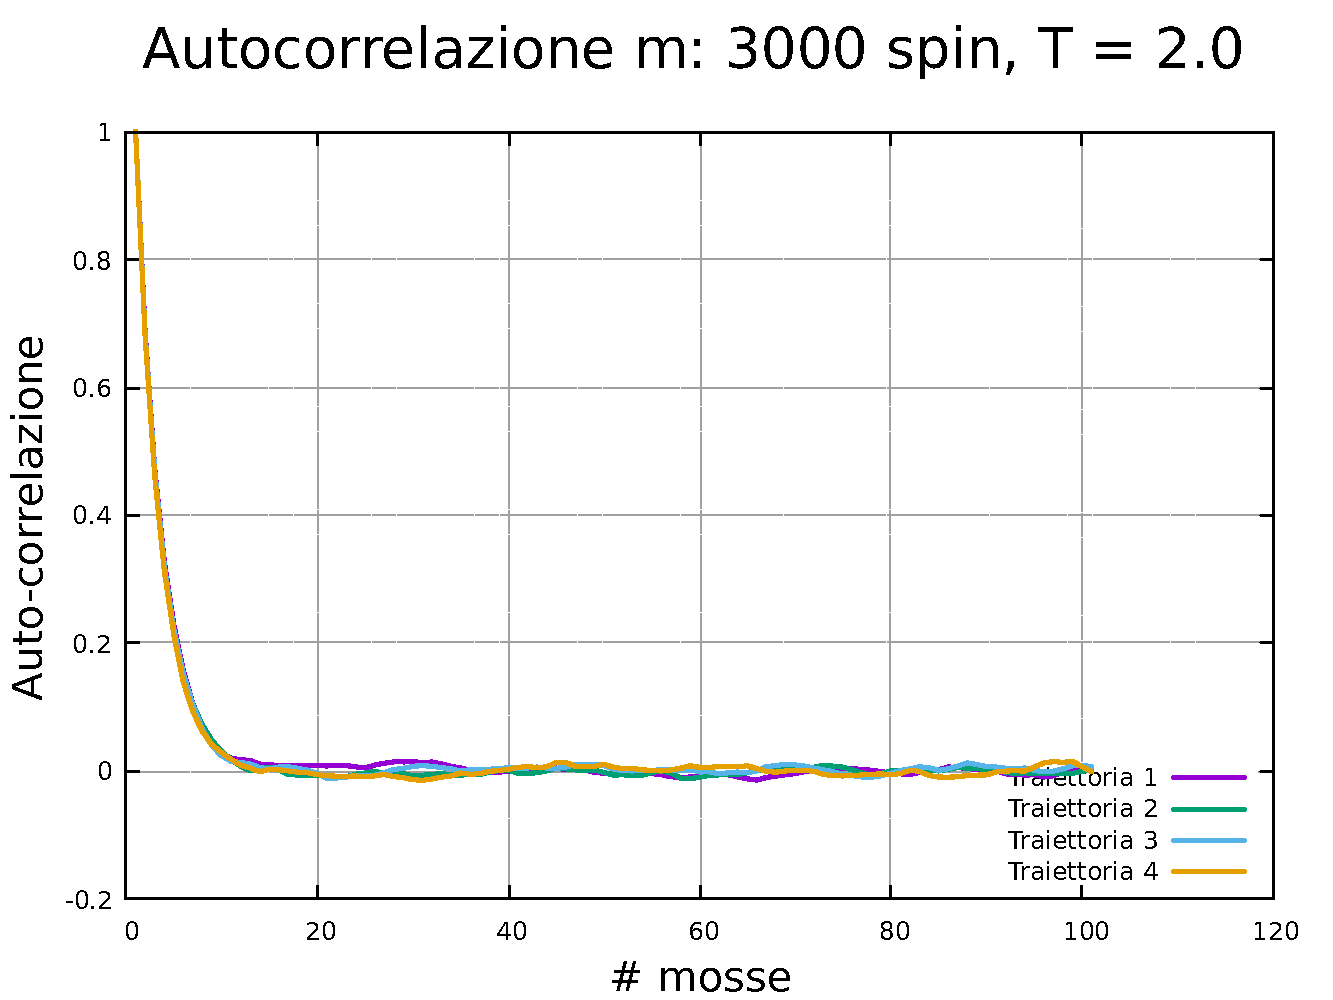
\includegraphics[page=1, width=\textwidth]{Immagini/simIsing1D/magn0.02/tcorr/tcorr_3000_2.0.pdf}
      \caption{$T\,=\,2.0$}
    \end{minipage}
    \caption{Studio dell'auto-correlazione per un modello di Ising 1D: $N_s$ = 3000, h = 0.02.}
\end{figure}

\vspace*{\fill}

\newpage

\vspace*{\fill}

\begin{figure}[htbp]
    \centering
    \begin{minipage}{0.45\textwidth}  
      \centering
      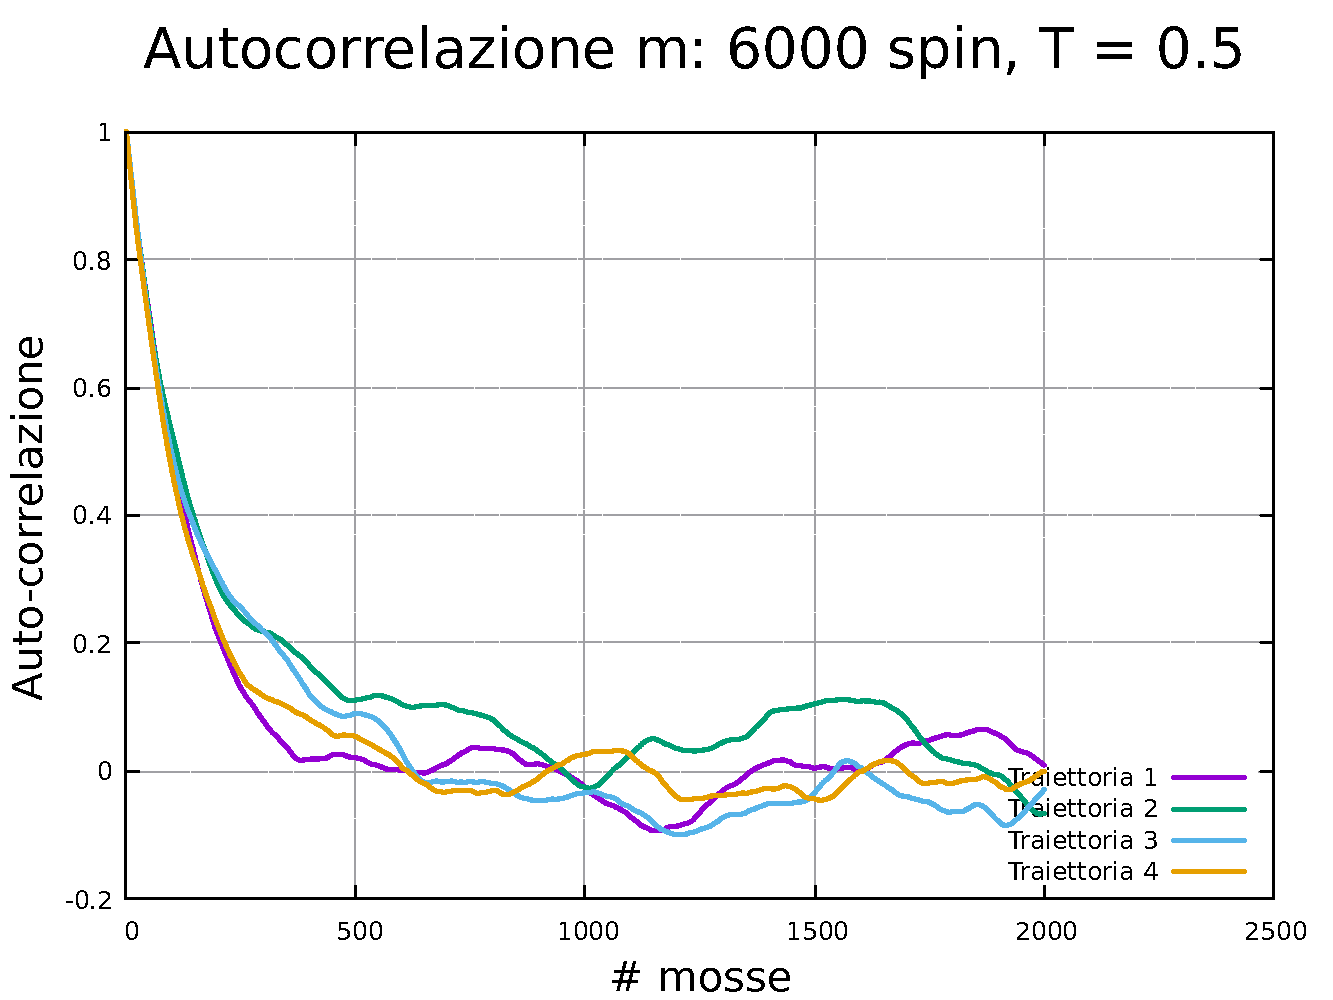
\includegraphics[page=1, width=\textwidth]{Immagini/simIsing1D/magn0.02/tcorr/tcorr_6000_0.5.pdf}
      \caption{$T\,=\,0.5$}
    \end{minipage}\hfill
    \begin{minipage}{0.45\textwidth}  
      \centering
      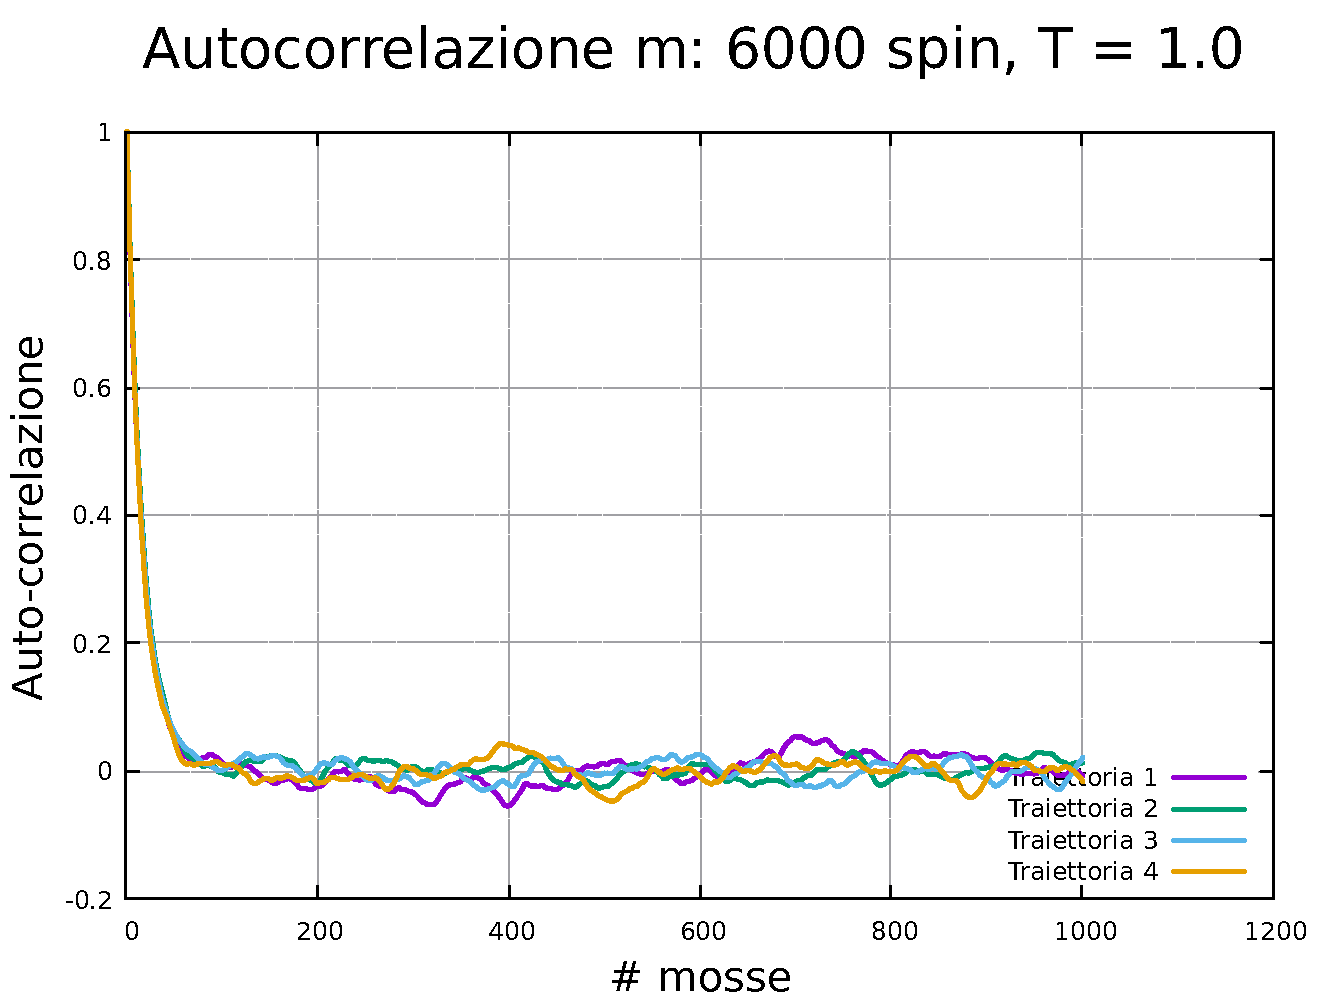
\includegraphics[page=1, width=\textwidth]{Immagini/simIsing1D/magn0.02/tcorr/tcorr_6000_1.0.pdf}
      \caption{$T\,=\,1.0$}
    \end{minipage}
    \vskip\baselineskip 
  
    \begin{minipage}{0.45\textwidth}  
      \centering
      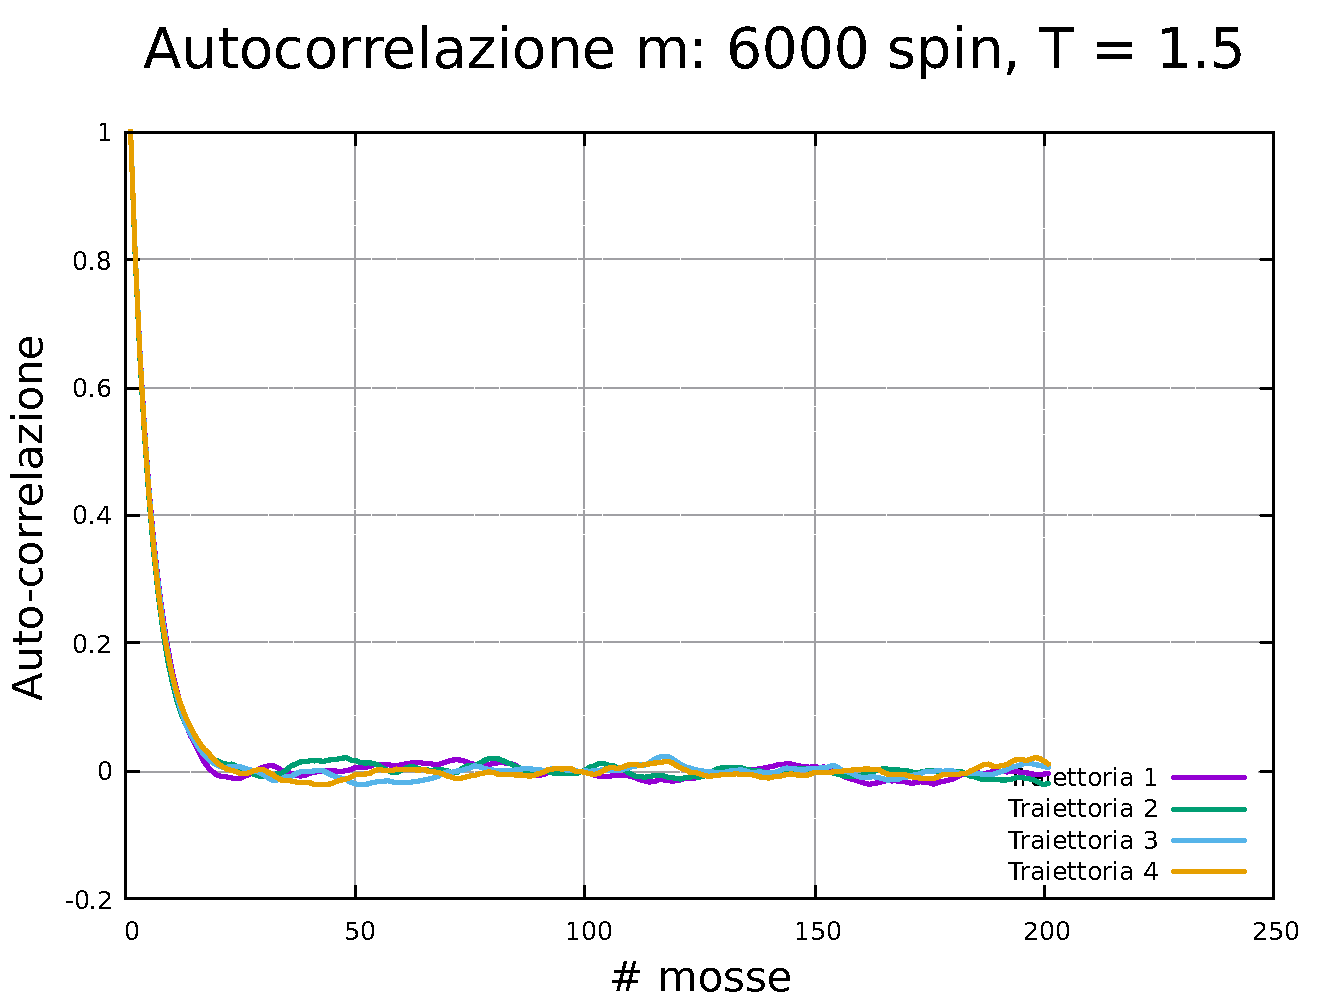
\includegraphics[page=1, width=\textwidth]{Immagini/simIsing1D/magn0.02/tcorr/tcorr_6000_1.5.pdf}
      \caption{$T\,=\,1.5$}
    \end{minipage}\hfill
    \begin{minipage}{0.45\textwidth}  
      \centering
      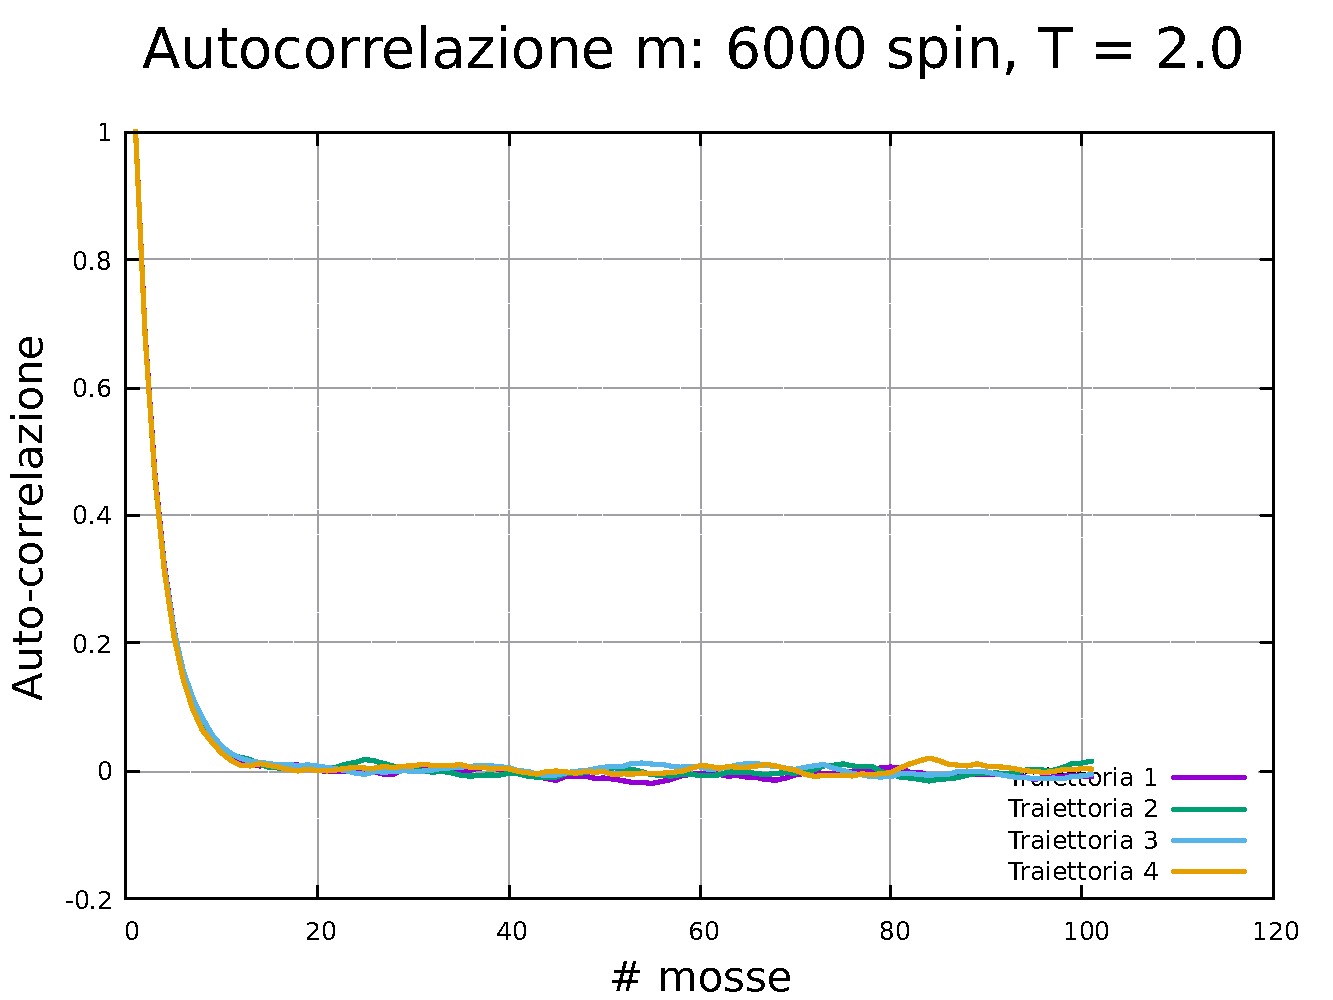
\includegraphics[page=1, width=\textwidth]{Immagini/simIsing1D/magn0.02/tcorr/tcorr_6000_2.0.pdf}
      \caption{$T\,=\,2.0$}
    \end{minipage}
    \caption{Studio dell'auto-correlazione per un modello di Ising 1D: $N_s$ = 6000, h = 0.02.}
\end{figure}

\vspace*{\fill}

\newpage

\vspace*{\fill}

\begin{figure}[htbp]
    \centering
    \begin{minipage}{0.45\textwidth}  
      \centering
      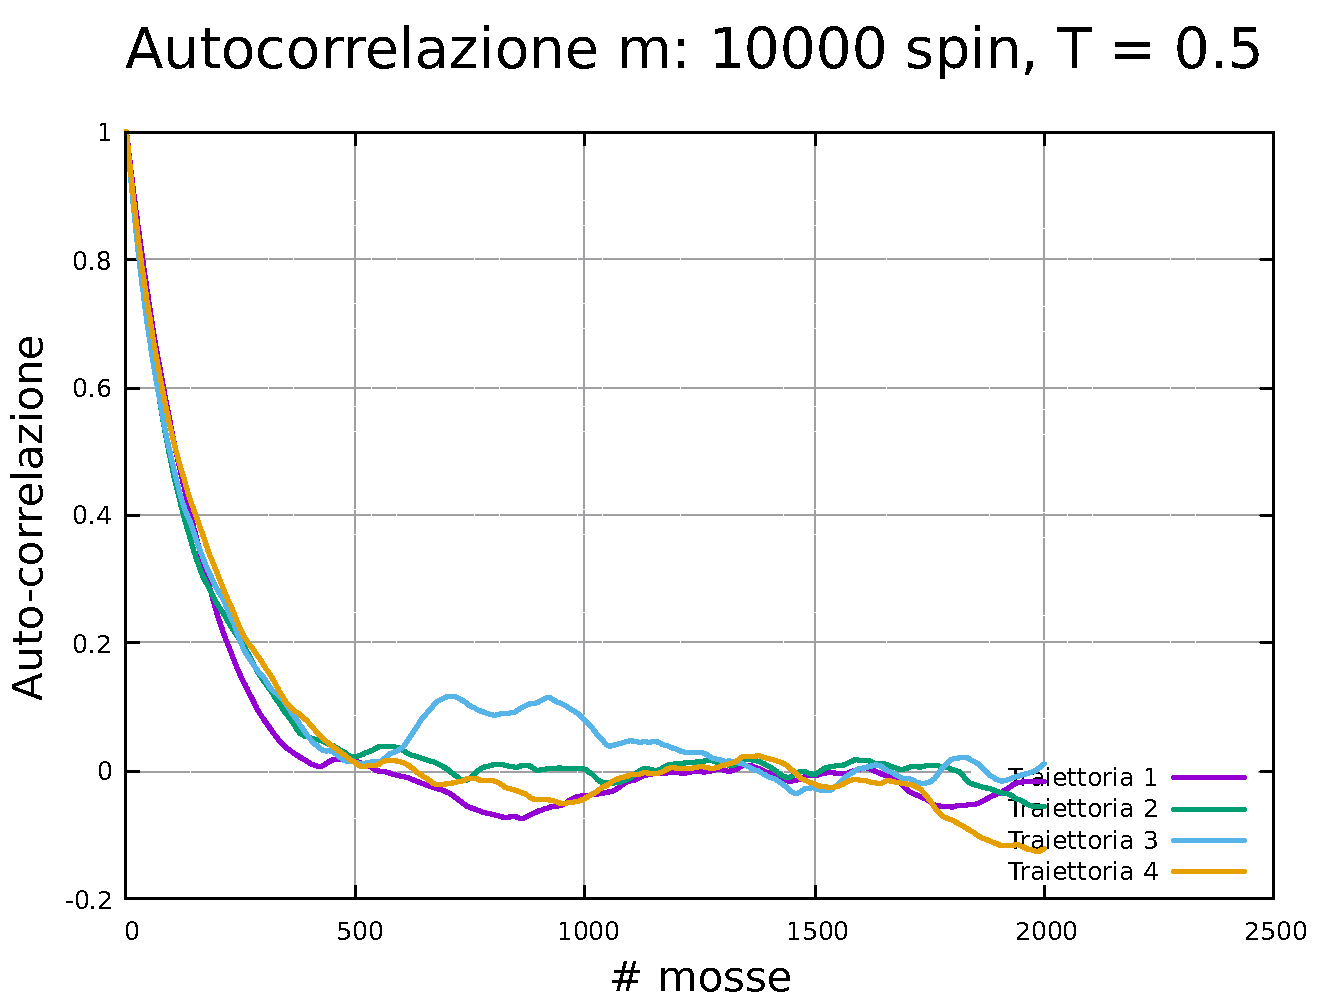
\includegraphics[page=1, width=\textwidth]{Immagini/simIsing1D/magn0.02/tcorr/tcorr_10000_0.5.pdf}
      \caption{$T\,=\,0.5$}
    \end{minipage}\hfill
    \begin{minipage}{0.45\textwidth}  
      \centering
      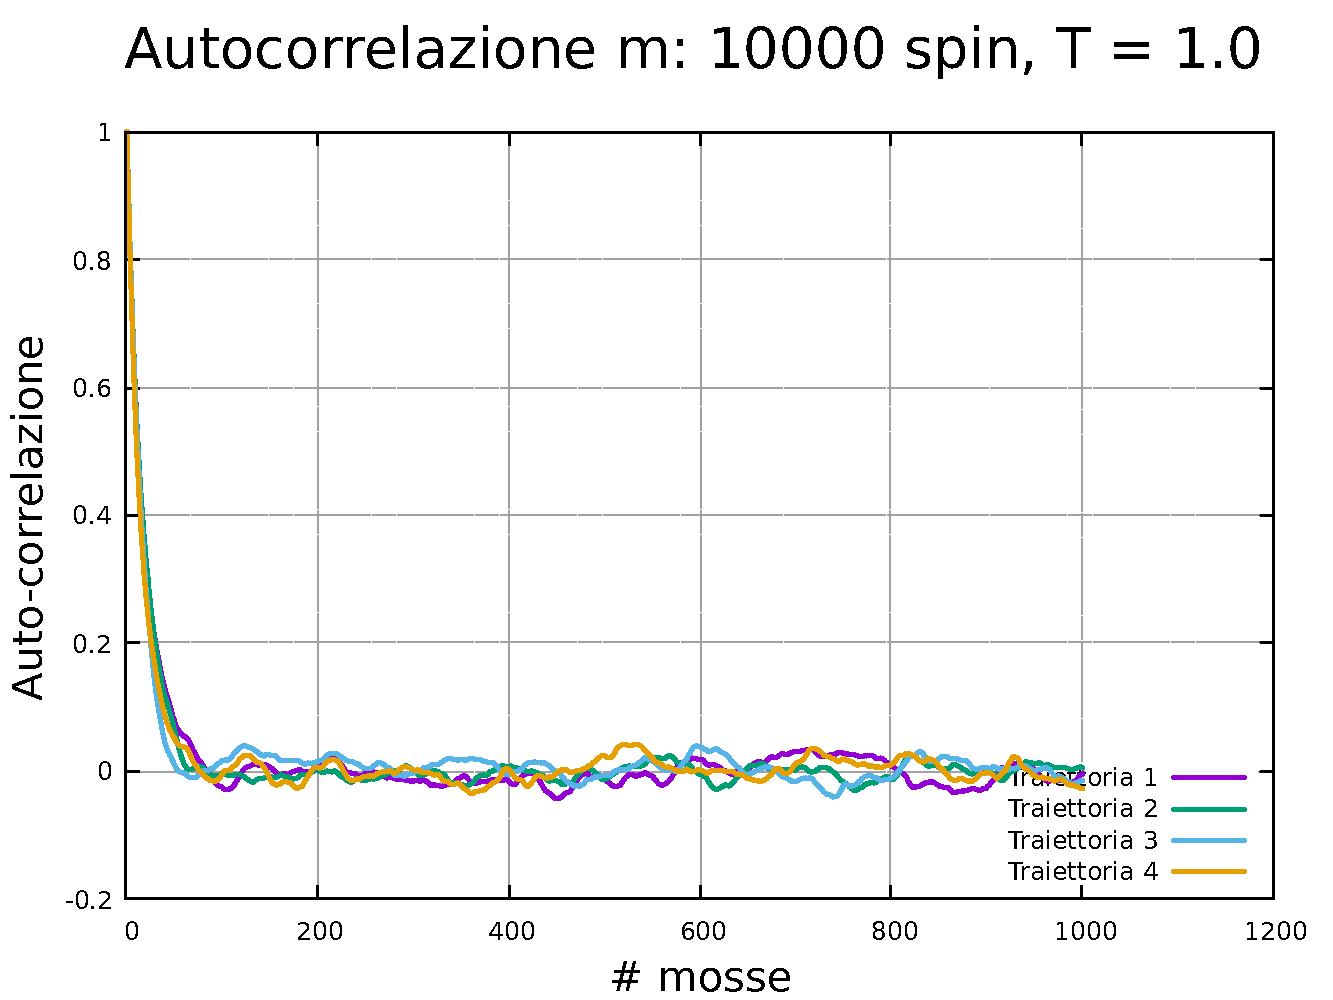
\includegraphics[page=1, width=\textwidth]{Immagini/simIsing1D/magn0.02/tcorr/tcorr_10000_1.0.pdf}
      \caption{$T\,=\,1.0$}
    \end{minipage}
    \vskip\baselineskip 
  
    \begin{minipage}{0.45\textwidth}  
      \centering
      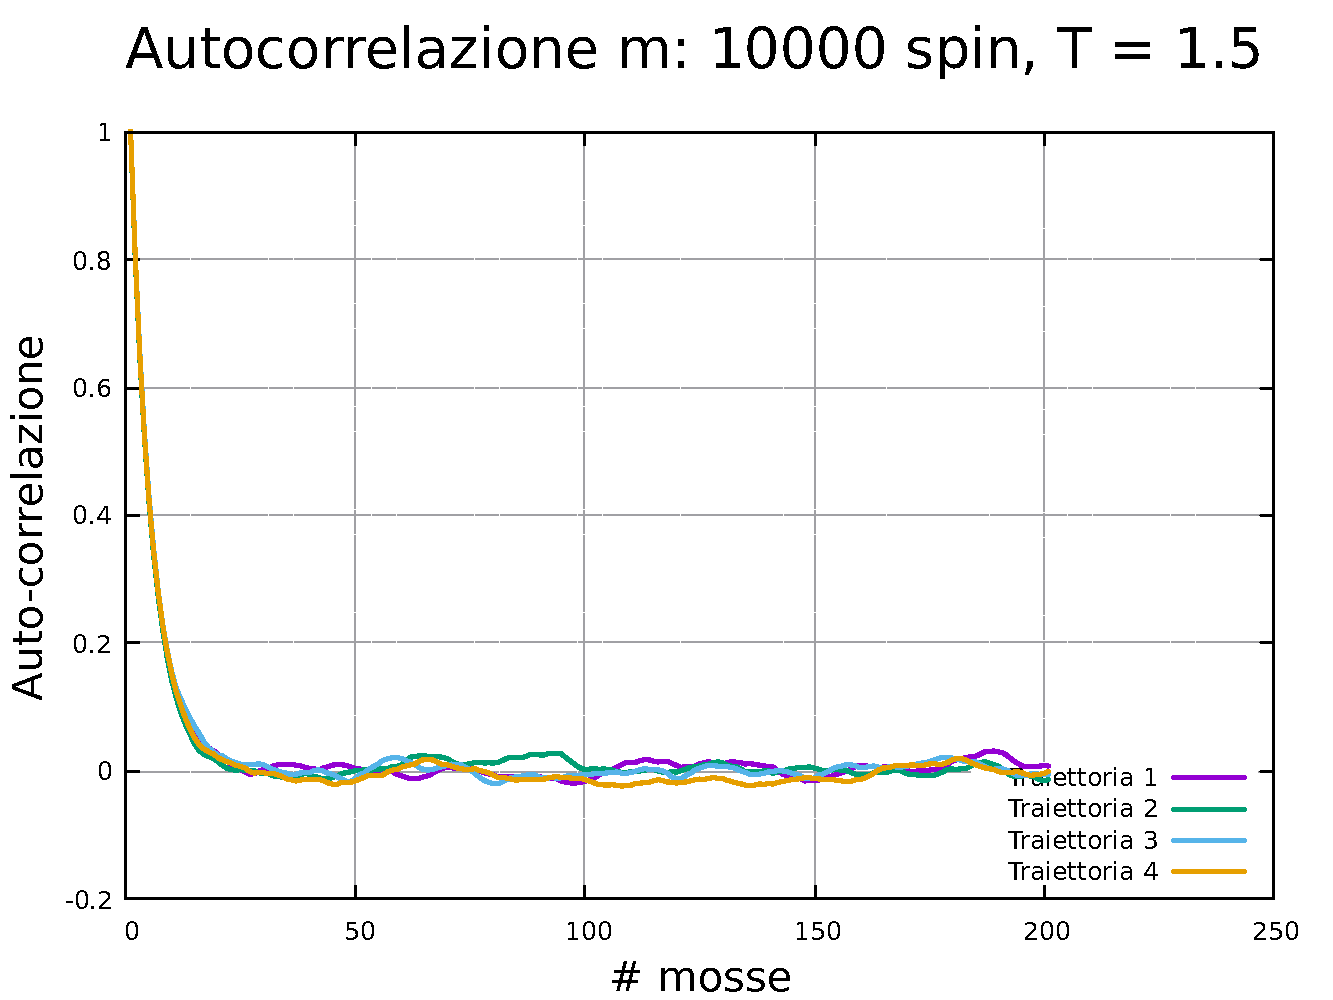
\includegraphics[page=1, width=\textwidth]{Immagini/simIsing1D/magn0.02/tcorr/tcorr_10000_1.5.pdf}
      \caption{$T\,=\,1.5$}
    \end{minipage}\hfill
    \begin{minipage}{0.45\textwidth}  
      \centering
      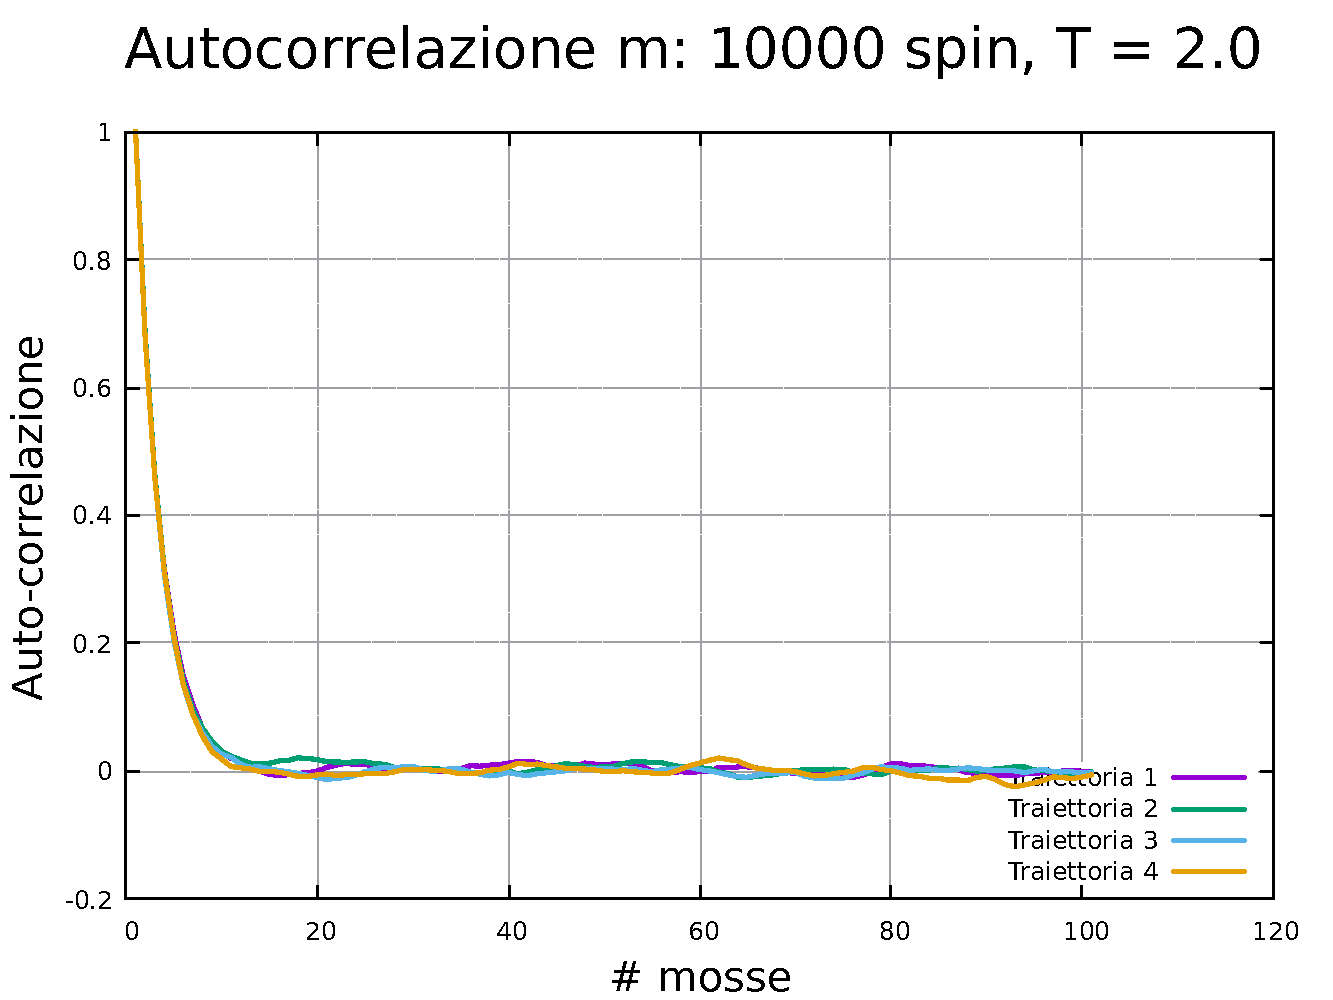
\includegraphics[page=1, width=\textwidth]{Immagini/simIsing1D/magn0.02/tcorr/tcorr_10000_2.0.pdf}
      \caption{$T\,=\,2.0$}
    \end{minipage}
    \caption{Studio dell'auto-correlazione per un modello di Ising 1D: $N_s$ = 10000, h = 0.02.}
\end{figure}

\vspace*{\fill}

\newpage



\subsection{Dimensione dei blocchi}

\vspace*{\fill}

\begin{figure}[htbp]
    \centering
    \begin{minipage}{0.45\textwidth}  
      \centering
      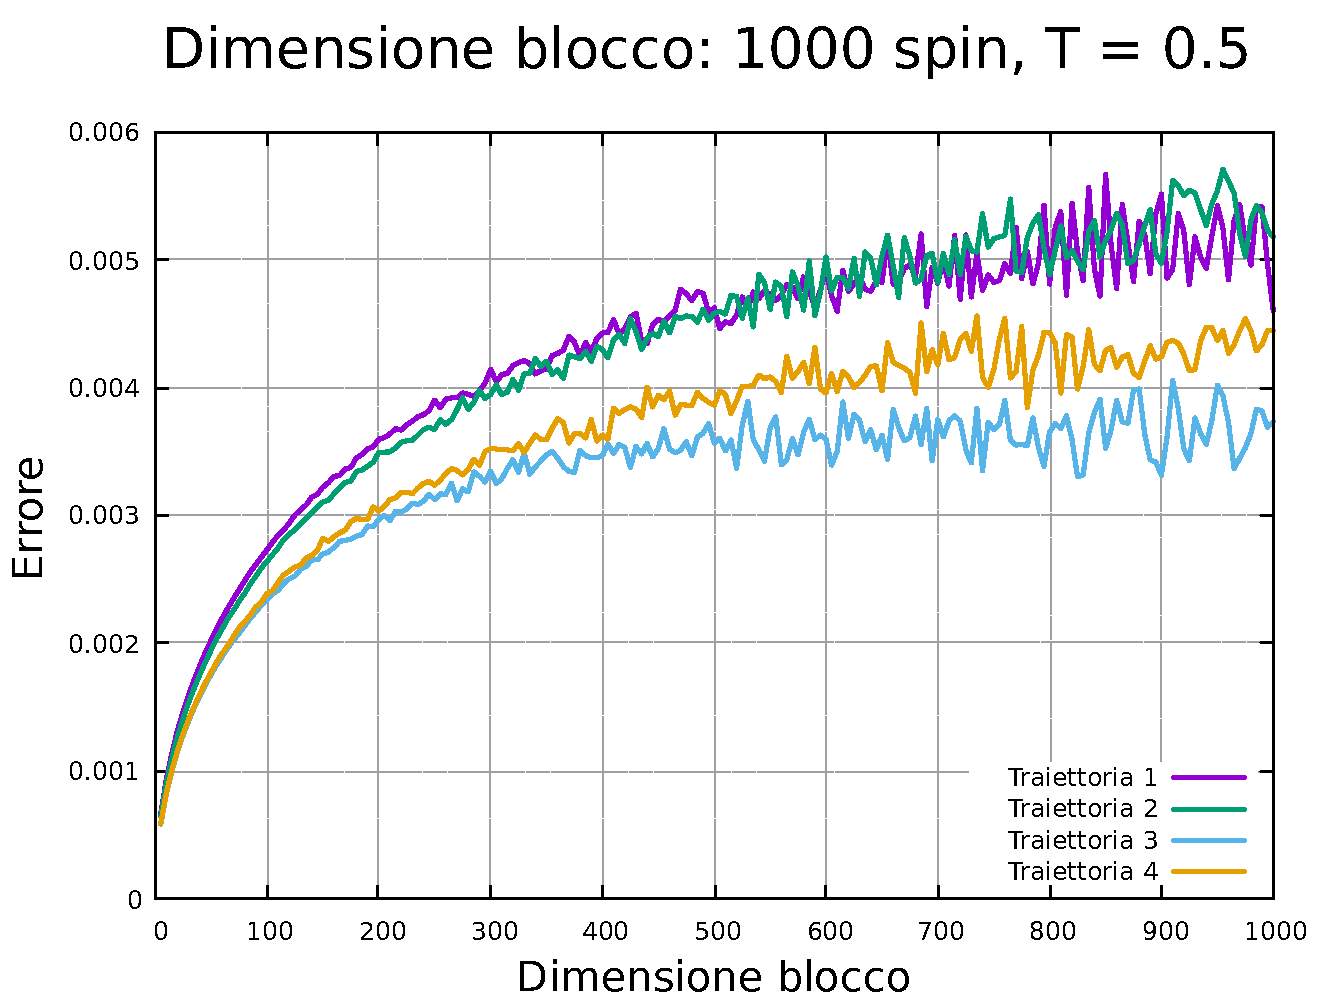
\includegraphics[page=1, width=\textwidth]{Immagini/simIsing1D/magn0.02/lblk/err_1000_0.5.pdf}
      \caption{$T\,=\,0.5$}
    \end{minipage}\hfill
    \begin{minipage}{0.45\textwidth}  
      \centering
      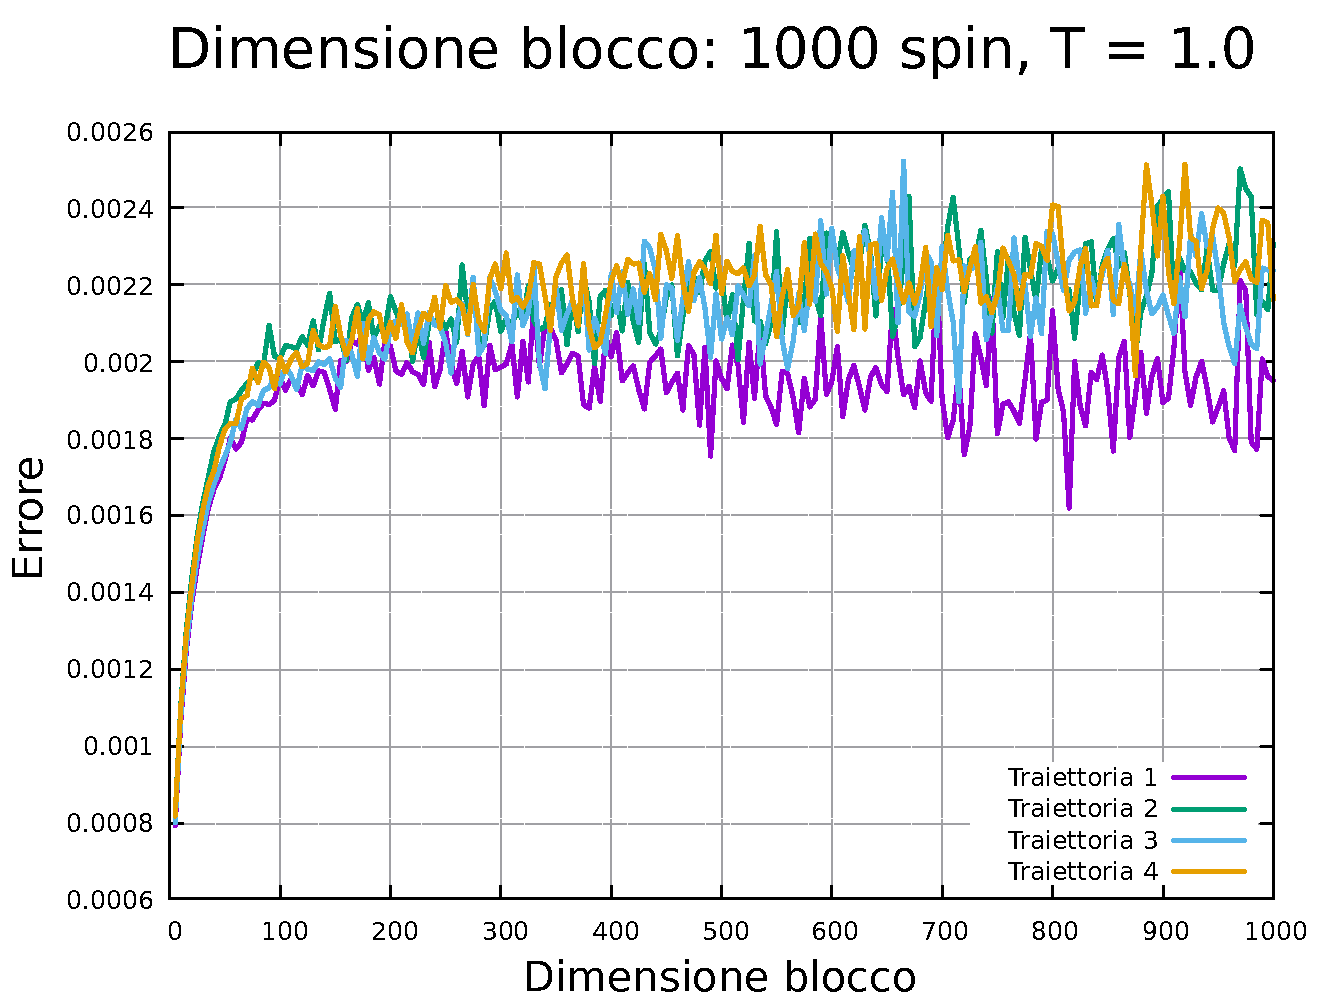
\includegraphics[page=1, width=\textwidth]{Immagini/simIsing1D/magn0.02/lblk/err_1000_1.0.pdf}
      \caption{$T\,=\,1.0$}
    \end{minipage}
    \vskip\baselineskip 
  
    \begin{minipage}{0.45\textwidth}  
      \centering
      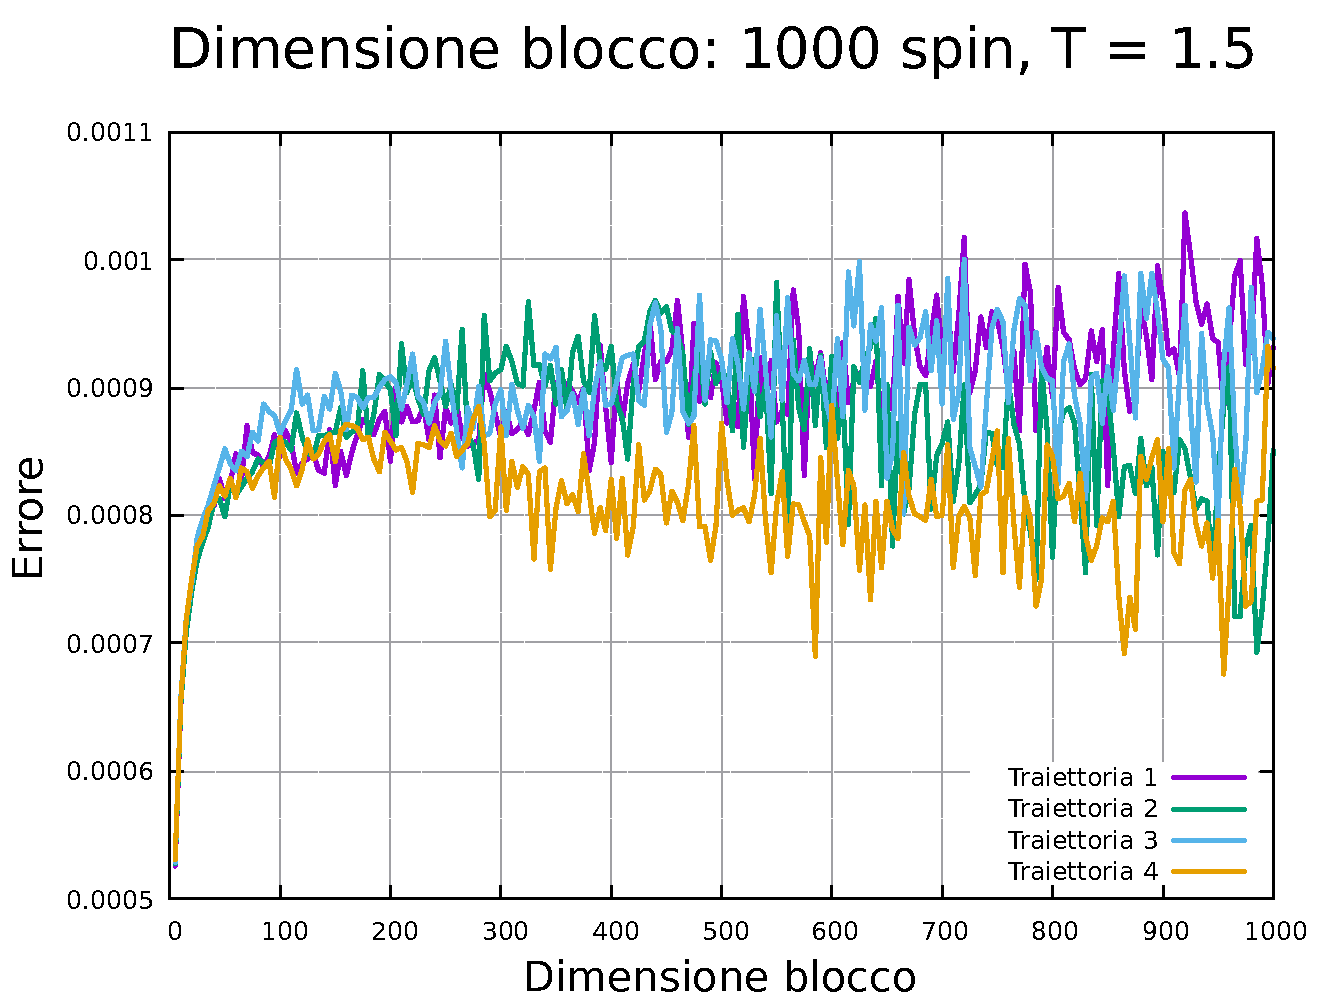
\includegraphics[page=1, width=\textwidth]{Immagini/simIsing1D/magn0.02/lblk/err_1000_1.5.pdf}
      \caption{$T\,=\,1.5$}
    \end{minipage}\hfill
    \begin{minipage}{0.45\textwidth}  
      \centering
      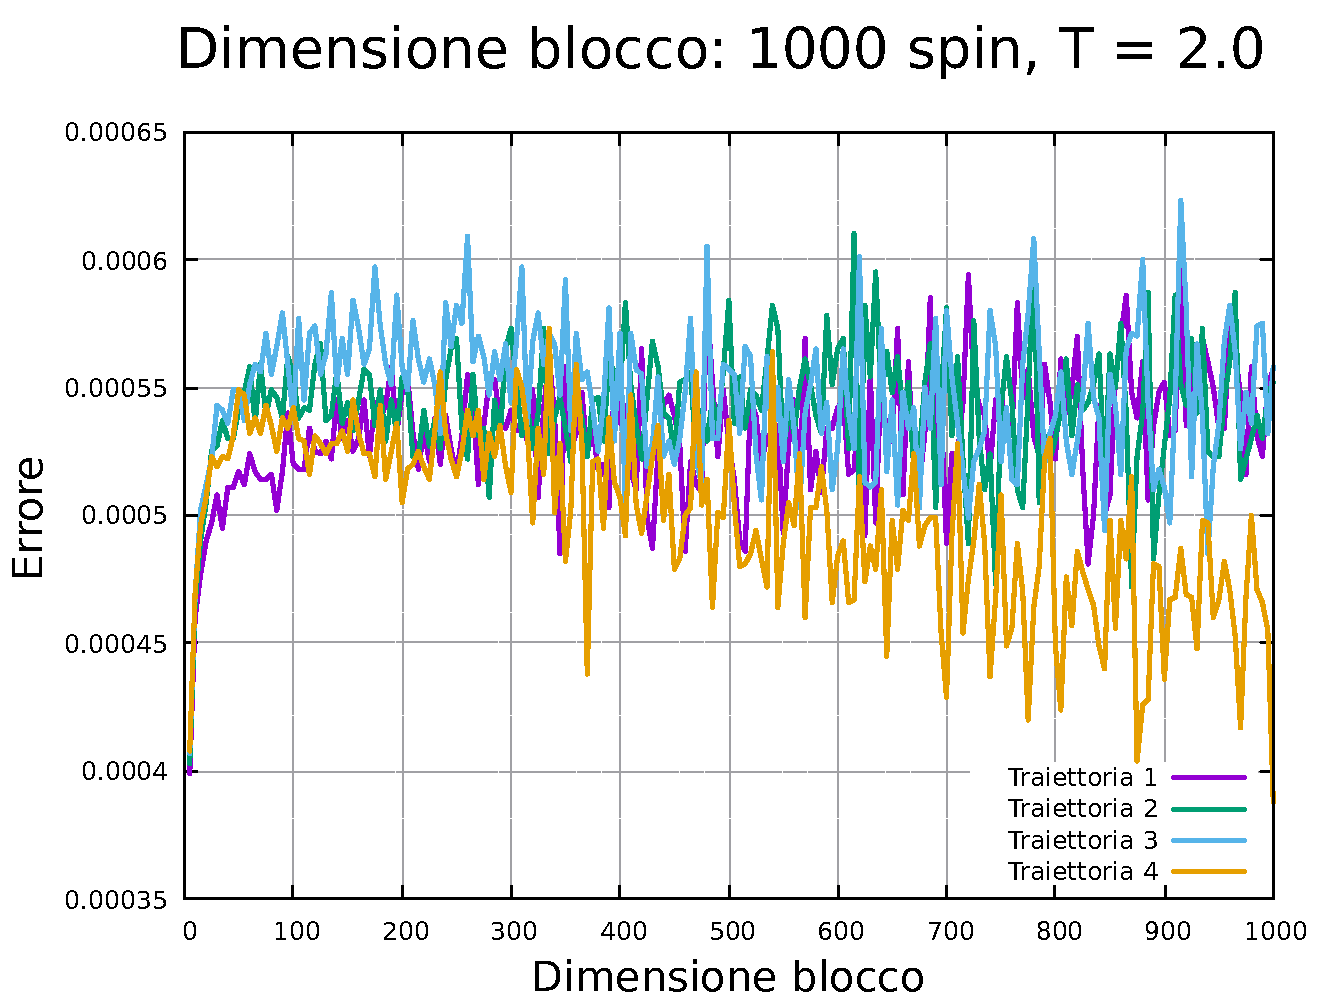
\includegraphics[page=1, width=\textwidth]{Immagini/simIsing1D/magn0.02/lblk/err_1000_2.0.pdf}
      \caption{$T\,=\,2.0$}
    \end{minipage}
    \caption{Errore in funzione della lunghezza dei blocchi per un modello di Ising 1D: $N_s$ = 1000, h = 0.02.}
\end{figure}

\vspace*{\fill}

\newpage

\vspace*{\fill}

\begin{figure}[htbp]
    \centering
    \begin{minipage}{0.45\textwidth}  
      \centering
      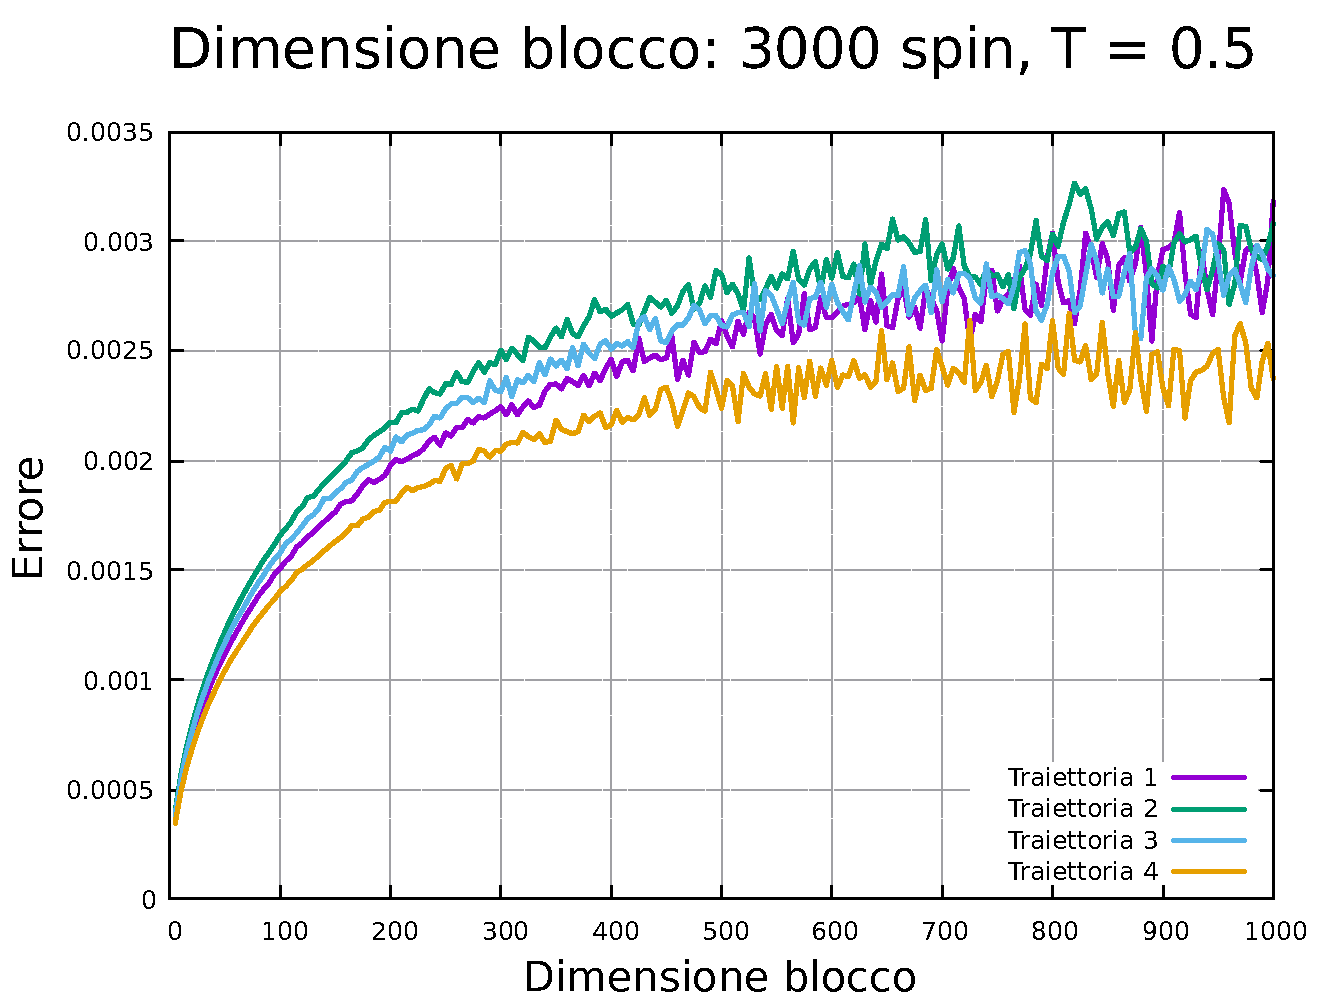
\includegraphics[page=1, width=\textwidth]{Immagini/simIsing1D/magn0.02/lblk/err_3000_0.5.pdf}
      \caption{$T\,=\,0.5$}
    \end{minipage}\hfill
    \begin{minipage}{0.45\textwidth}  
      \centering
      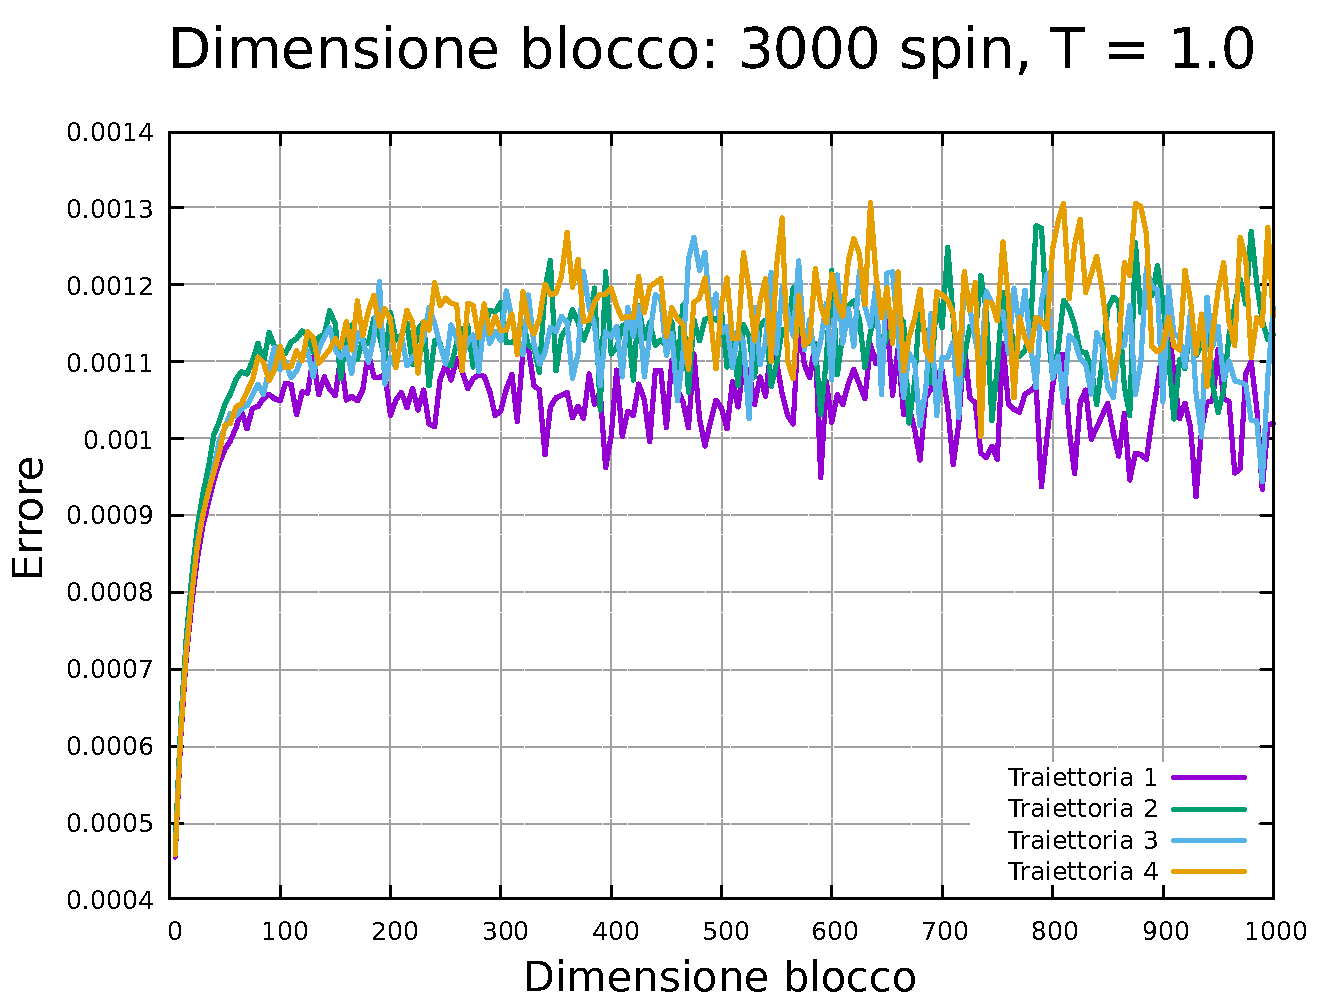
\includegraphics[page=1, width=\textwidth]{Immagini/simIsing1D/magn0.02/lblk/err_3000_1.0.pdf}
      \caption{$T\,=\,1.0$}
    \end{minipage}
    \vskip\baselineskip 
  
    \begin{minipage}{0.45\textwidth}  
      \centering
      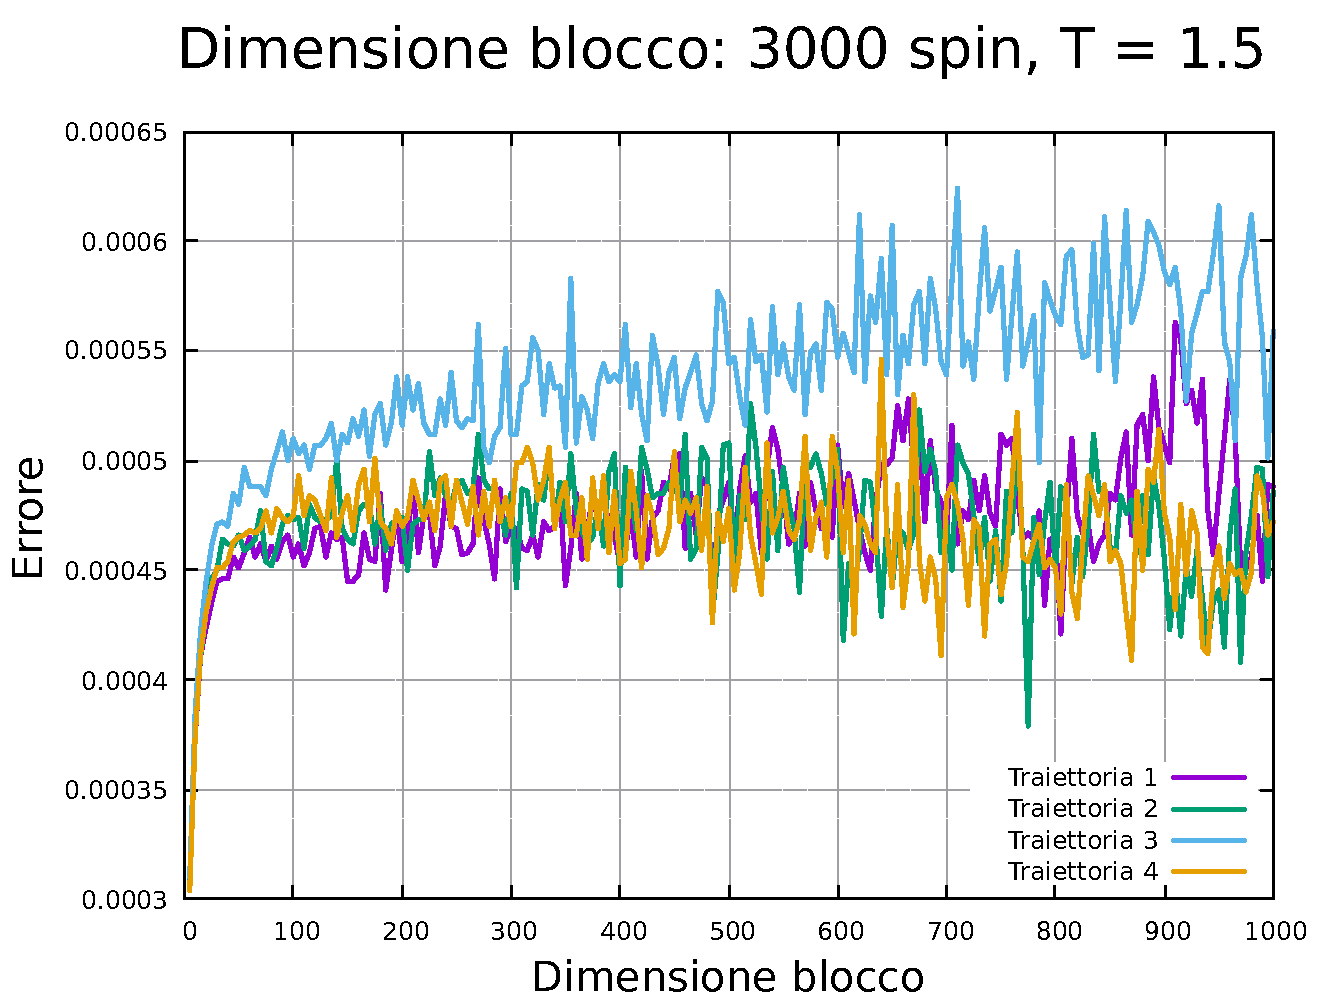
\includegraphics[page=1, width=\textwidth]{Immagini/simIsing1D/magn0.02/lblk/err_3000_1.5.pdf}
      \caption{$T\,=\,1.5$}
    \end{minipage}\hfill
    \begin{minipage}{0.45\textwidth}  
      \centering
      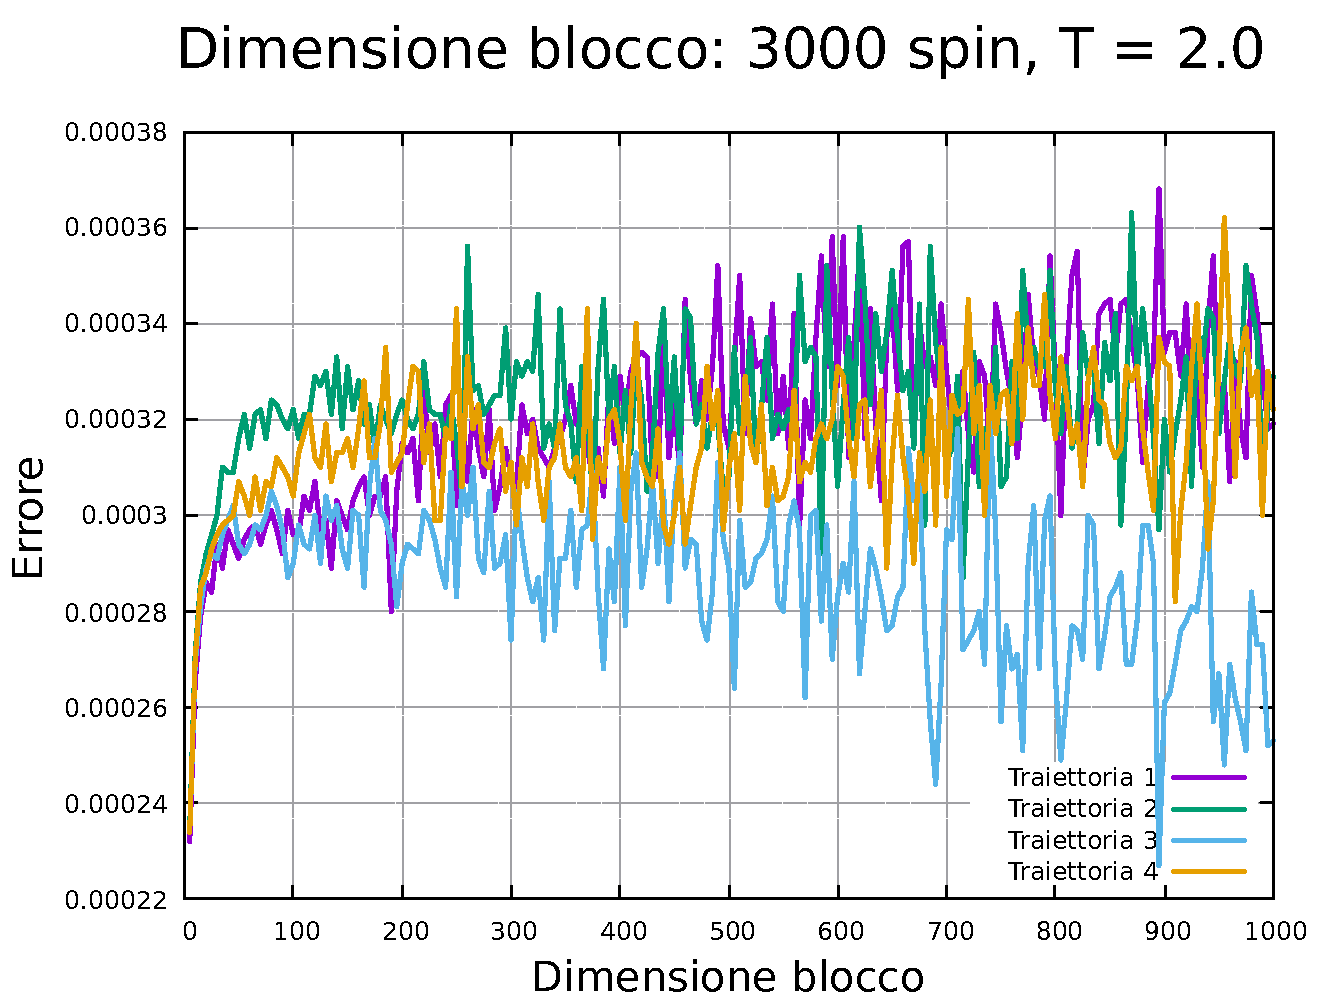
\includegraphics[page=1, width=\textwidth]{Immagini/simIsing1D/magn0.02/lblk/err_3000_2.0.pdf}
      \caption{$T\,=\,2.0$}
    \end{minipage}
    \caption{Errore in funzione della lunghezza dei blocchi per un modello di Ising 1D: $N_s$ = 3000, h = 0.02.}
\end{figure}

\vspace*{\fill}

\newpage

\vspace*{\fill}

\begin{figure}[htbp]
    \centering
    \begin{minipage}{0.45\textwidth}  
      \centering
      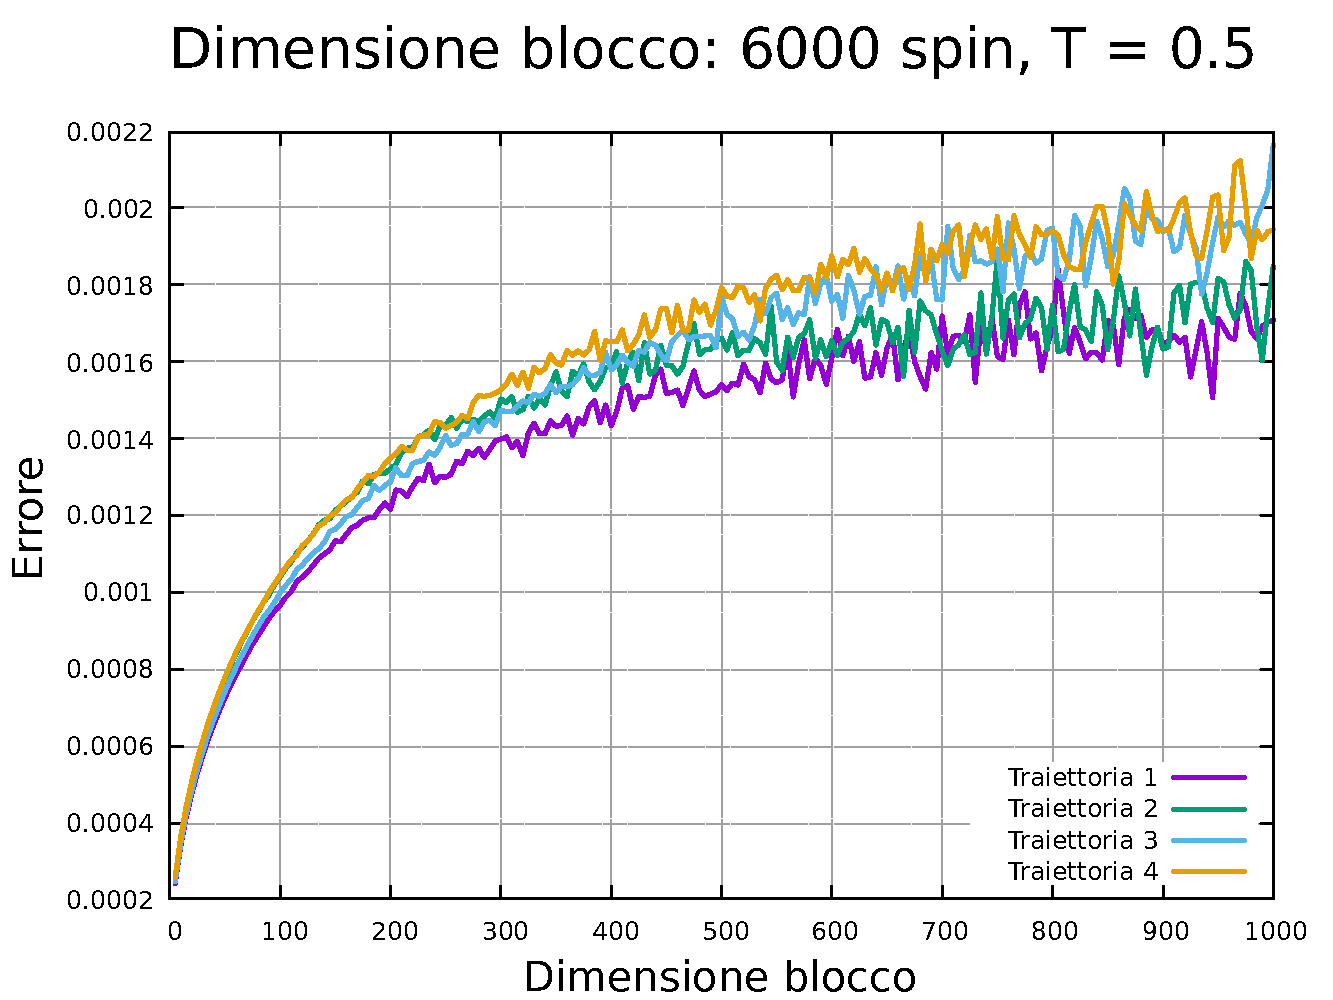
\includegraphics[page=1, width=\textwidth]{Immagini/simIsing1D/magn0.02/lblk/err_6000_0.5.pdf}
      \caption{$T\,=\,0.5$}
    \end{minipage}\hfill
    \begin{minipage}{0.45\textwidth}  
      \centering
      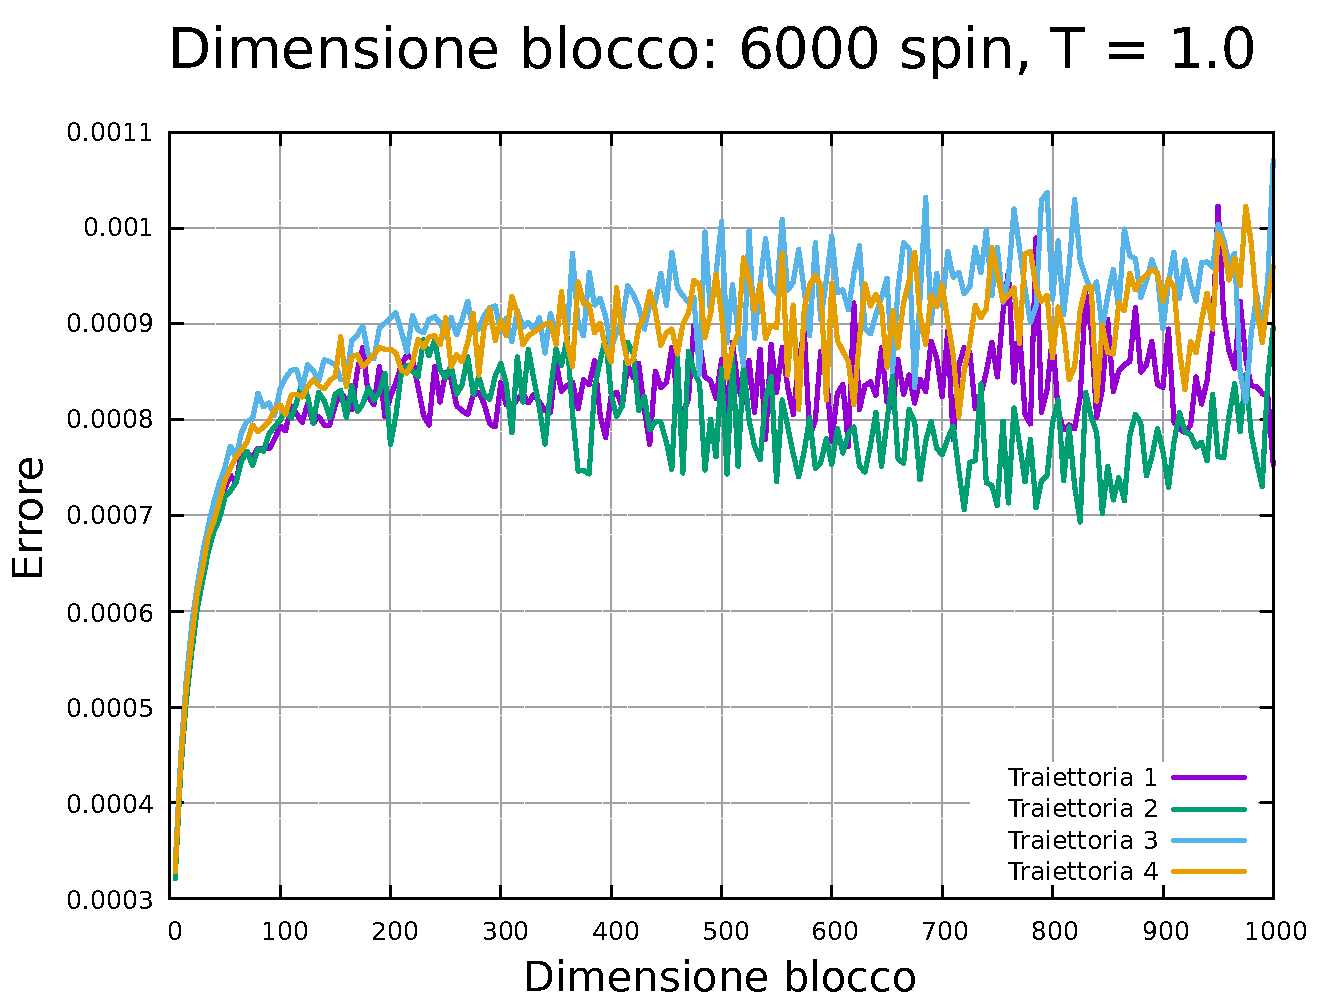
\includegraphics[page=1, width=\textwidth]{Immagini/simIsing1D/magn0.02/lblk/err_6000_1.0.pdf}
      \caption{$T\,=\,1.0$}
    \end{minipage}
    \vskip\baselineskip 
  
    \begin{minipage}{0.45\textwidth}  
      \centering
      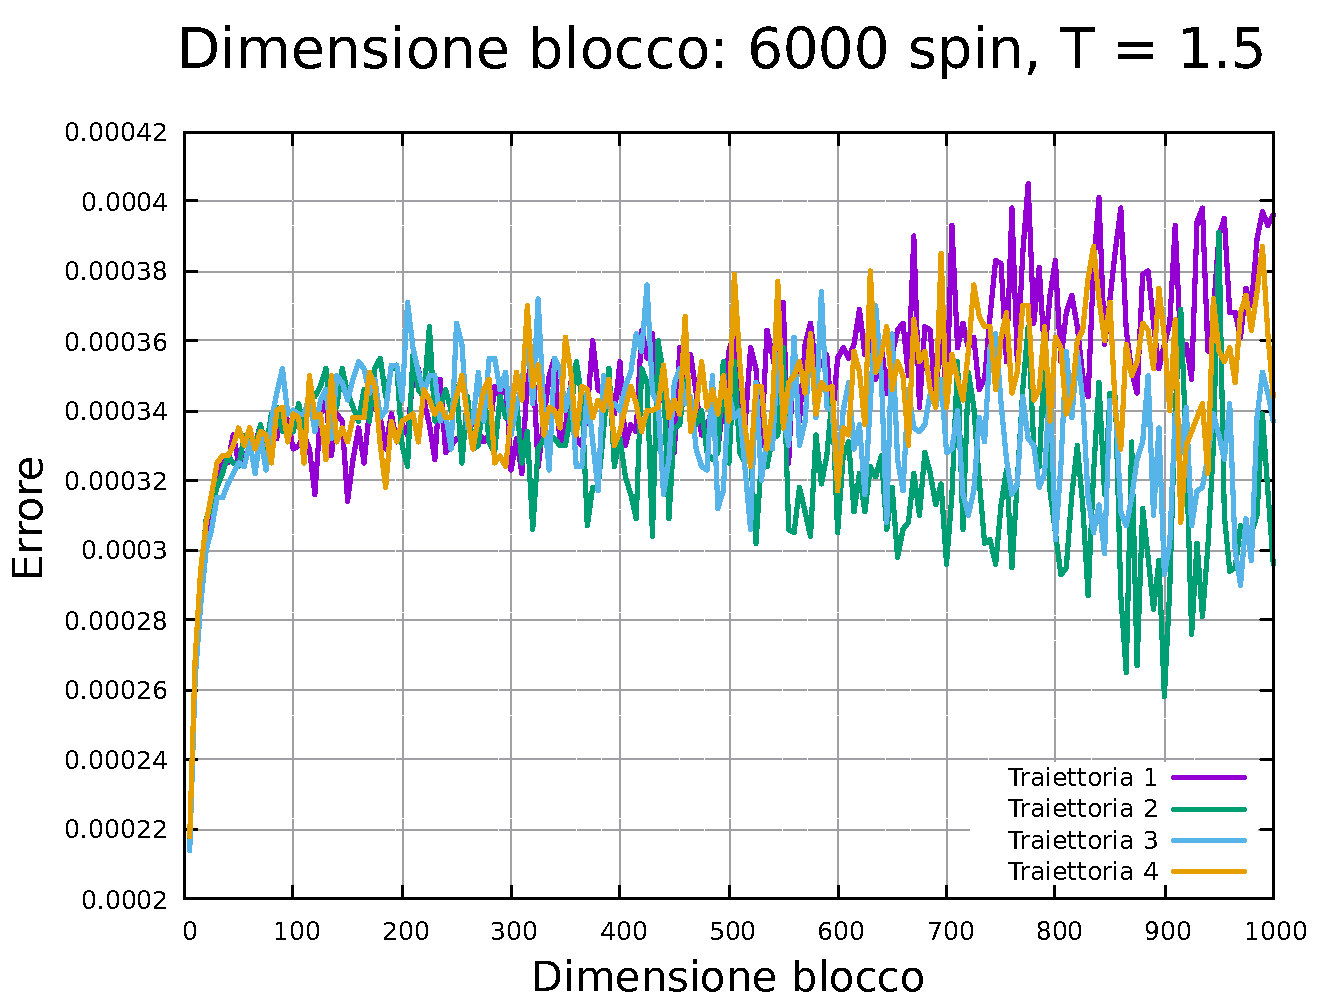
\includegraphics[page=1, width=\textwidth]{Immagini/simIsing1D/magn0.02/lblk/err_6000_1.5.pdf}
      \caption{$T\,=\,1.5$}
    \end{minipage}\hfill
    \begin{minipage}{0.45\textwidth}  
      \centering
      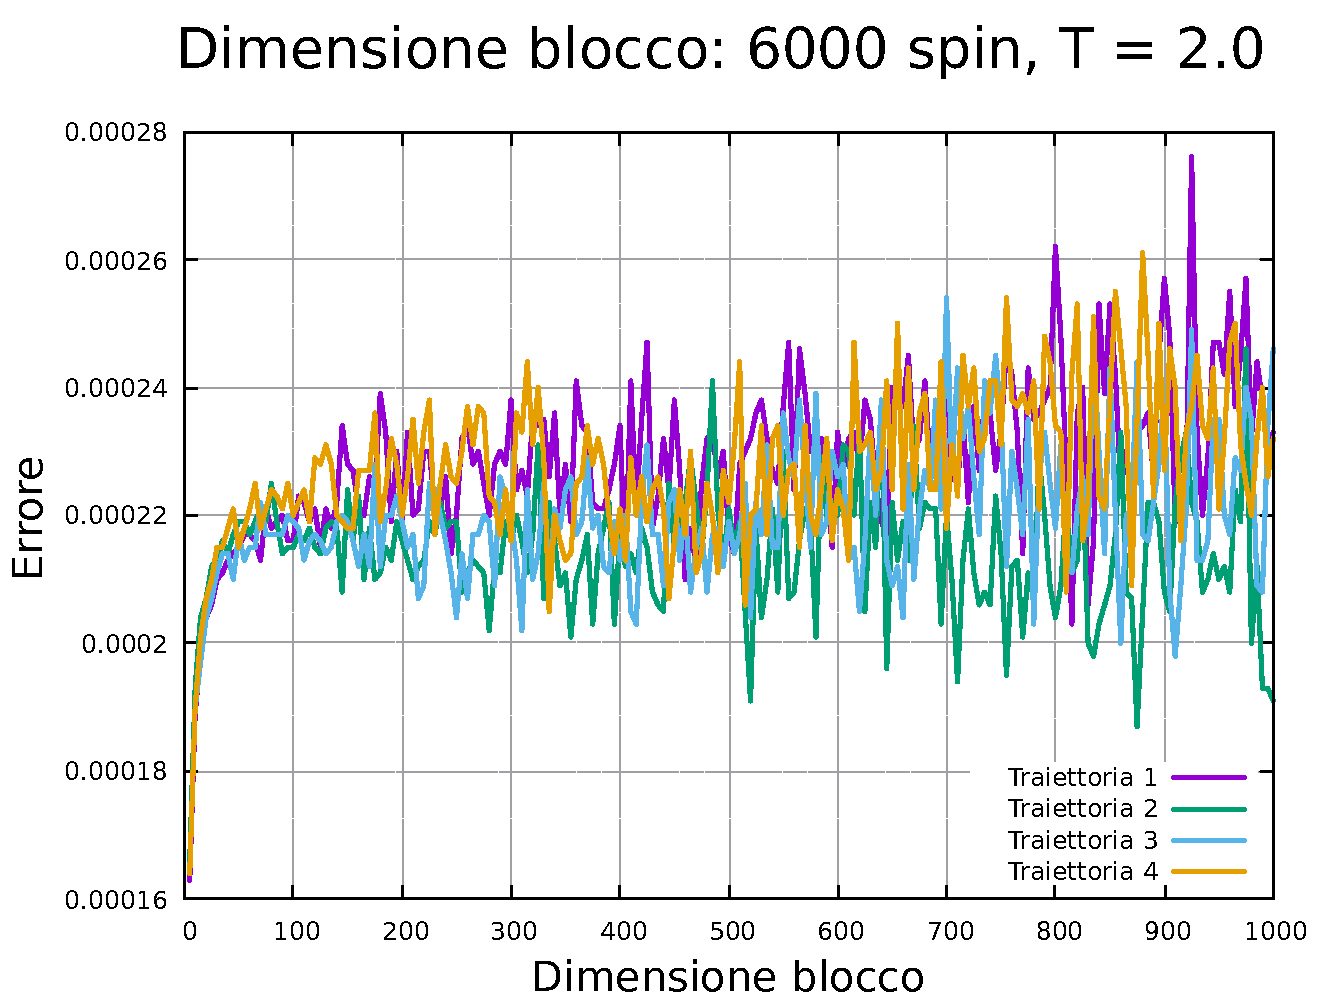
\includegraphics[page=1, width=\textwidth]{Immagini/simIsing1D/magn0.02/lblk/err_6000_2.0.pdf}
      \caption{$T\,=\,2.0$}
    \end{minipage}
    \caption{Errore in funzione della lunghezza dei blocchi per un modello di Ising 1D: $N_s$ = 6000, h = 0.02.}
\end{figure}

\vspace*{\fill}

\newpage

\vspace*{\fill}

\begin{figure}[htbp]
    \centering
    \begin{minipage}{0.45\textwidth}  
      \centering
      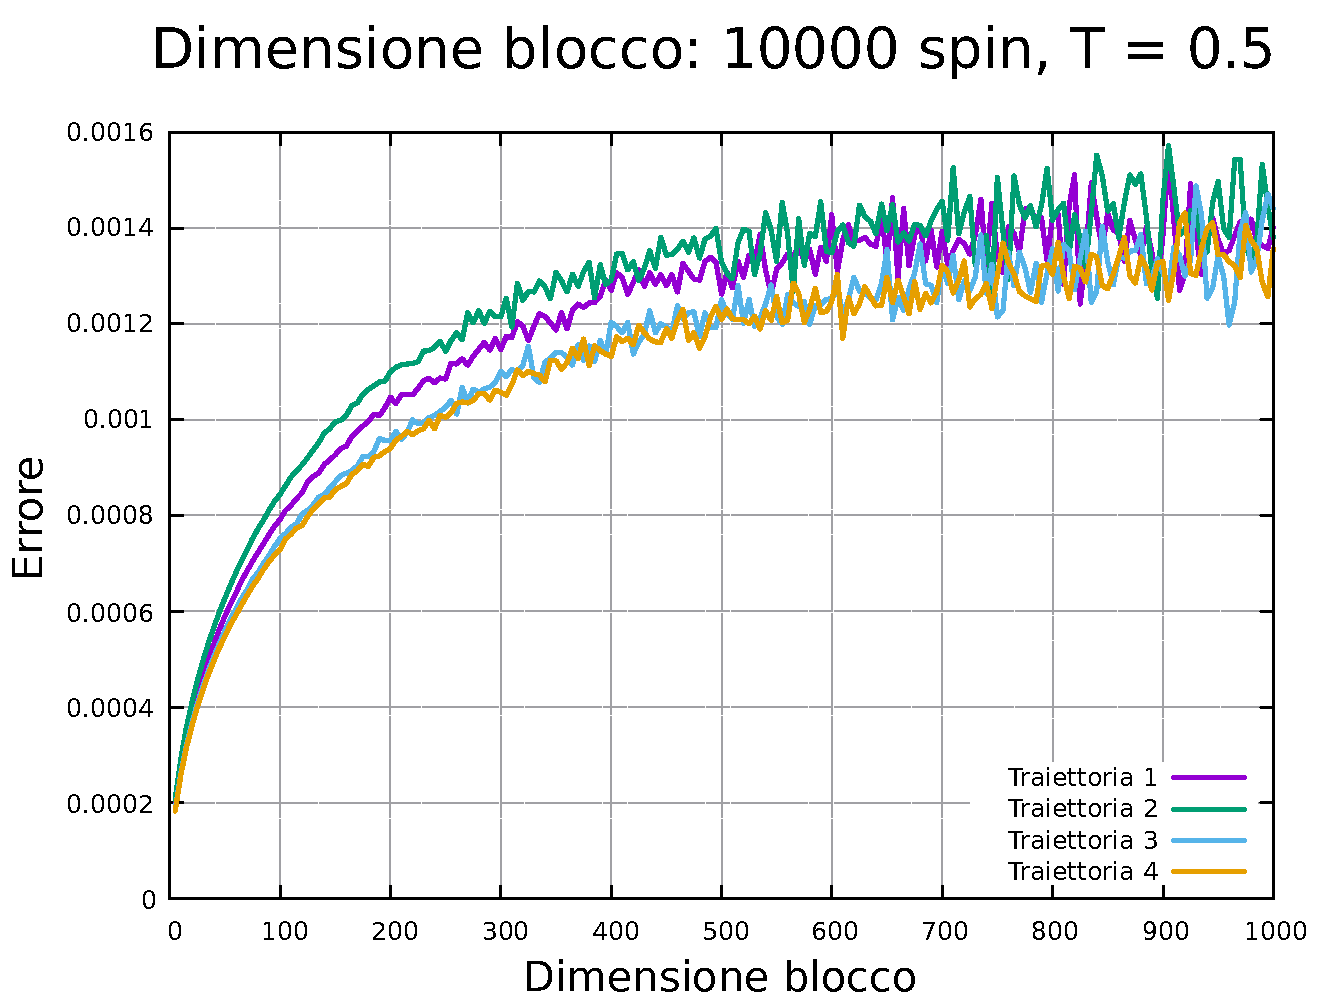
\includegraphics[page=1, width=\textwidth]{Immagini/simIsing1D/magn0.02/lblk/err_10000_0.5.pdf}
      \caption{$T\,=\,0.5$}
    \end{minipage}\hfill
    \begin{minipage}{0.45\textwidth}  
      \centering
      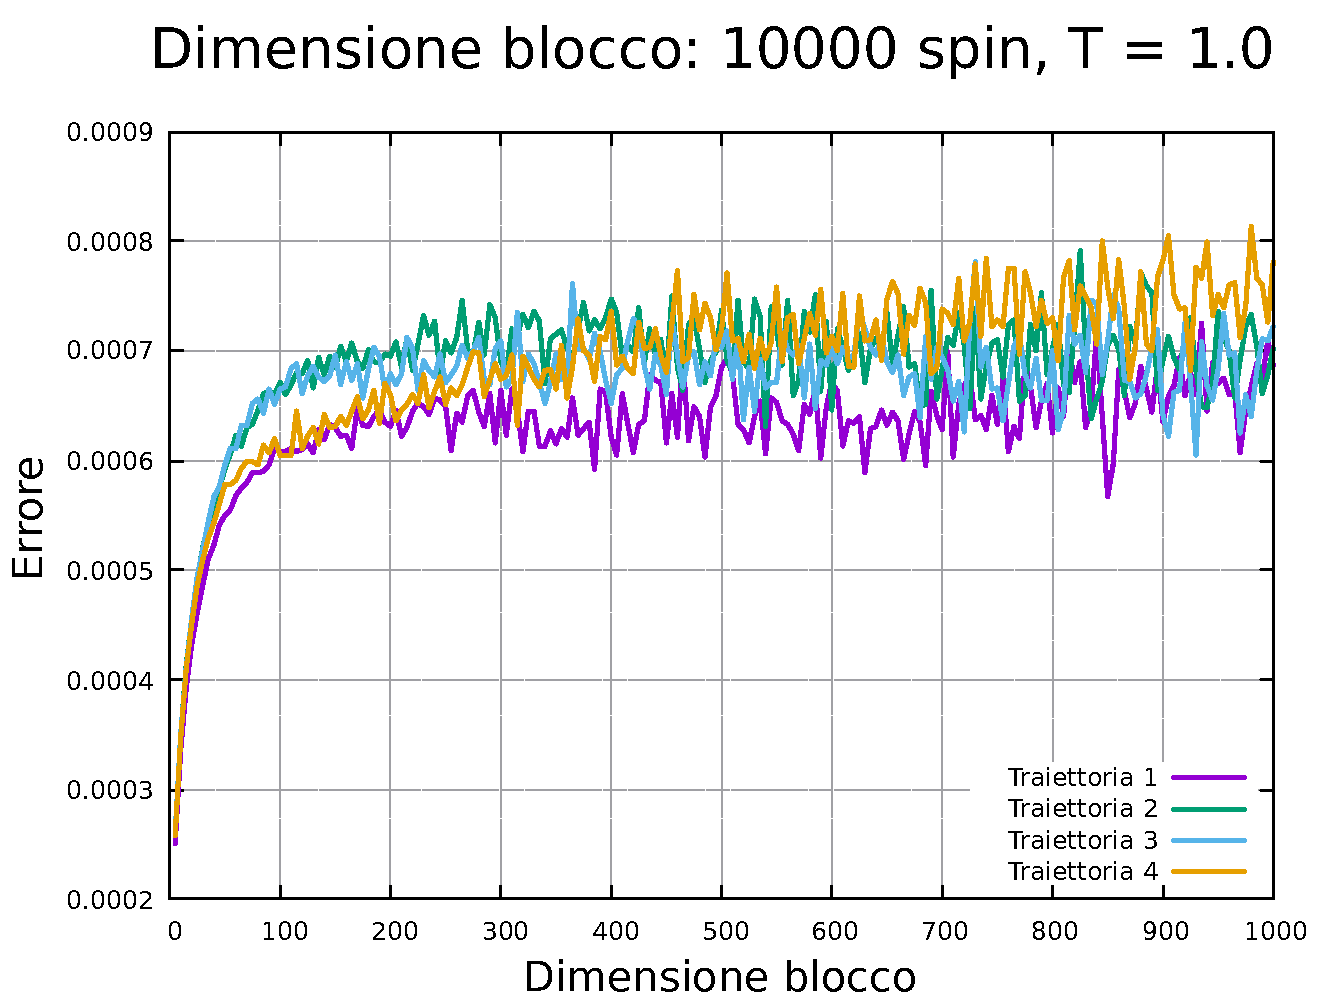
\includegraphics[page=1, width=\textwidth]{Immagini/simIsing1D/magn0.02/lblk/err_10000_1.0.pdf}
      \caption{$T\,=\,1.0$}
    \end{minipage}
    \vskip\baselineskip 
  
    \begin{minipage}{0.45\textwidth}  
      \centering
      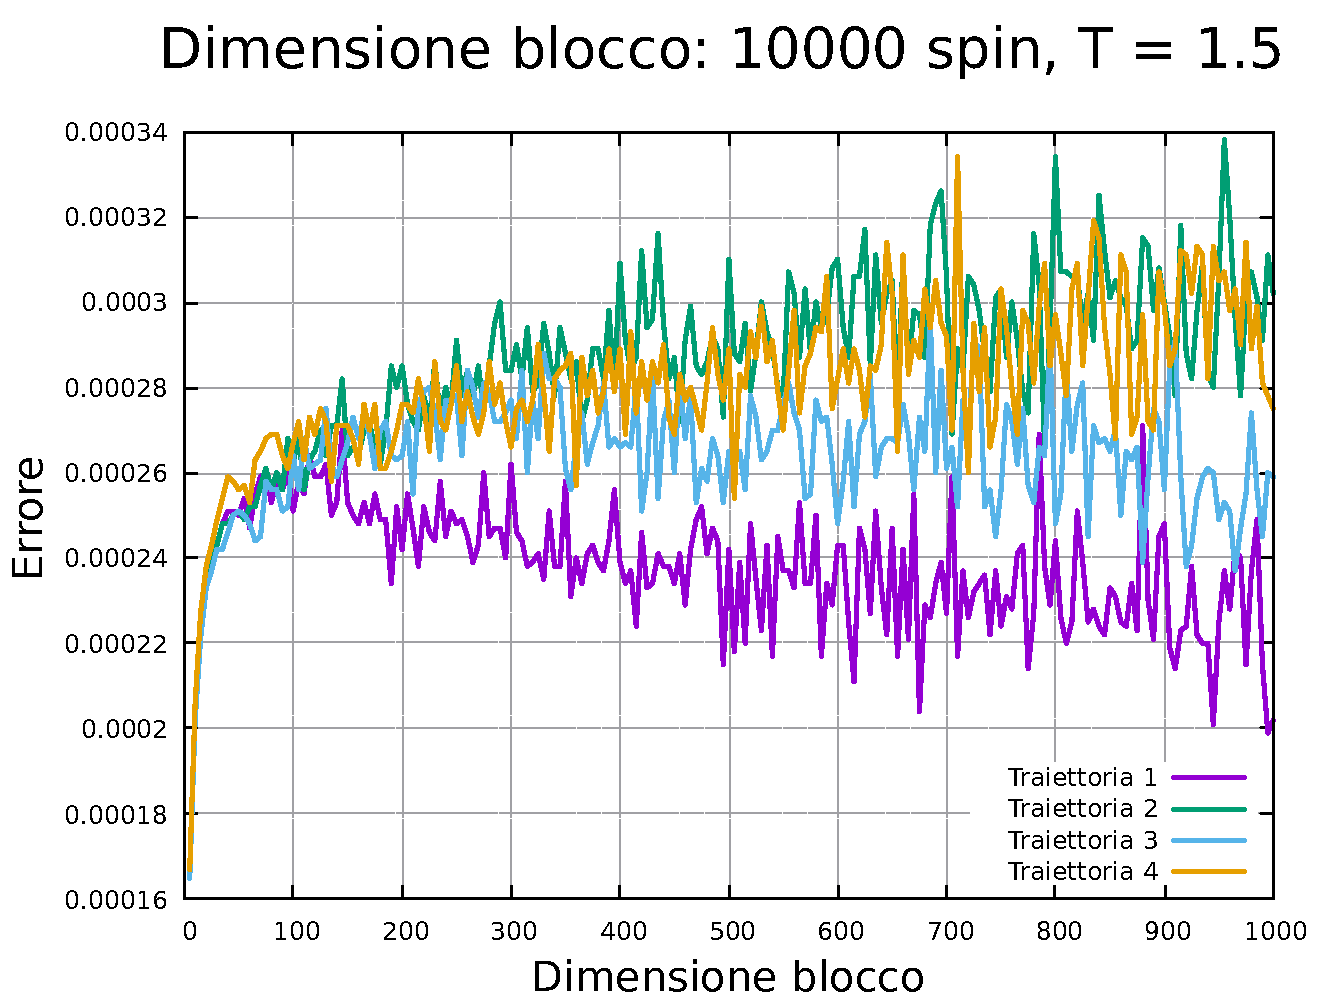
\includegraphics[page=1, width=\textwidth]{Immagini/simIsing1D/magn0.02/lblk/err_10000_1.5.pdf}
      \caption{$T\,=\,1.5$}
    \end{minipage}\hfill
    \begin{minipage}{0.45\textwidth}  
      \centering
      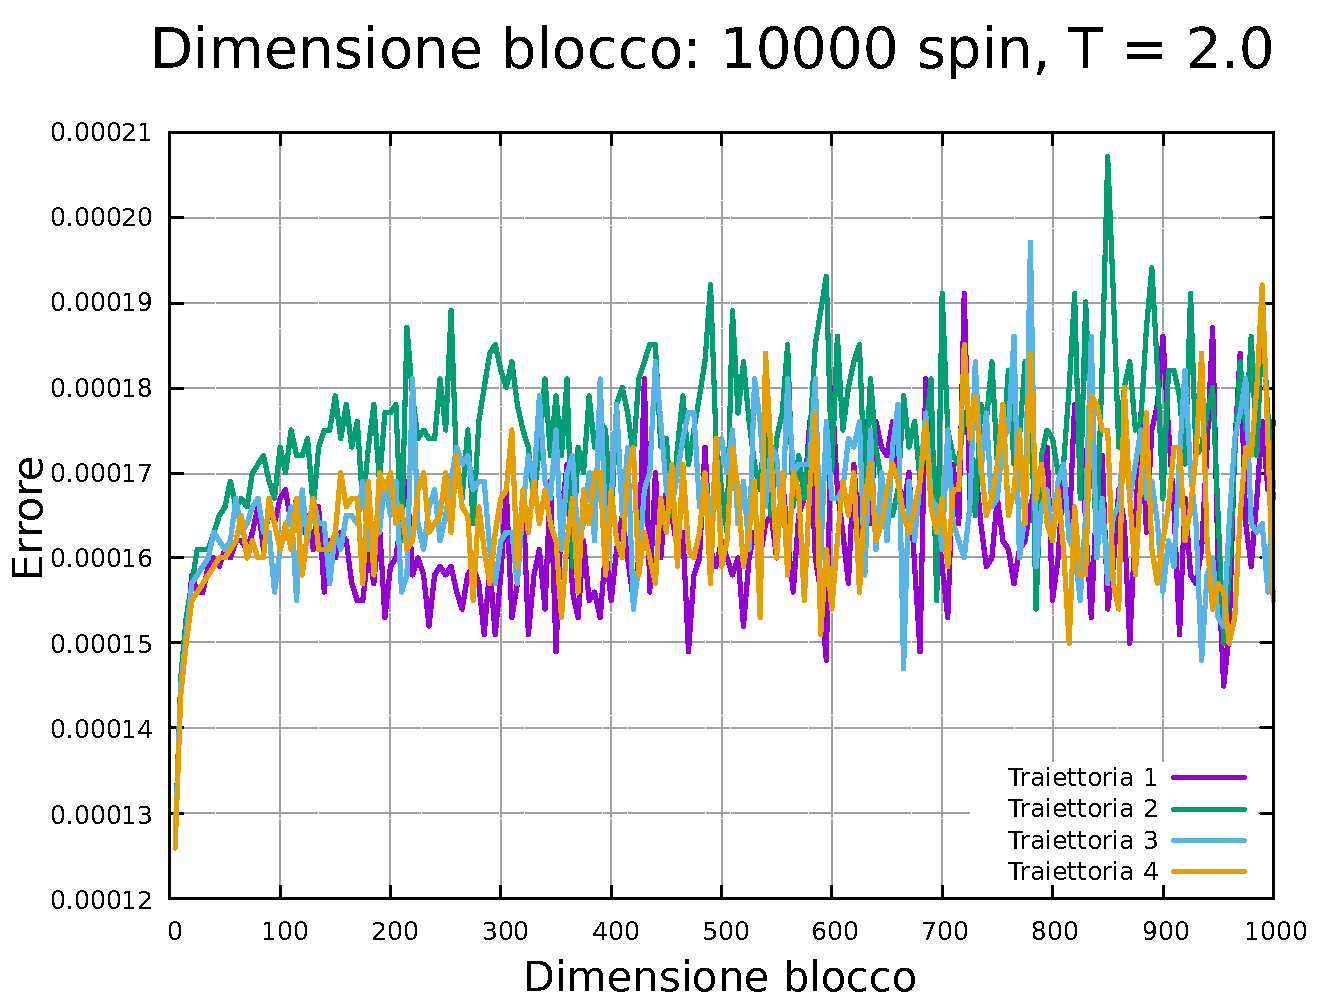
\includegraphics[page=1, width=\textwidth]{Immagini/simIsing1D/magn0.02/lblk/err_10000_2.0.pdf}
      \caption{$T\,=\,2.0$}
    \end{minipage}
    \caption{Errore in funzione della lunghezza dei blocchi per un modello di Ising 1D: $N_s$ = 10000, h = 0.02.}
\end{figure}

\vspace*{\fill}

\newpage



\subsection{Osservabili}

\vspace*{\fill}

\begin{figure}[htbp]
    \centering
    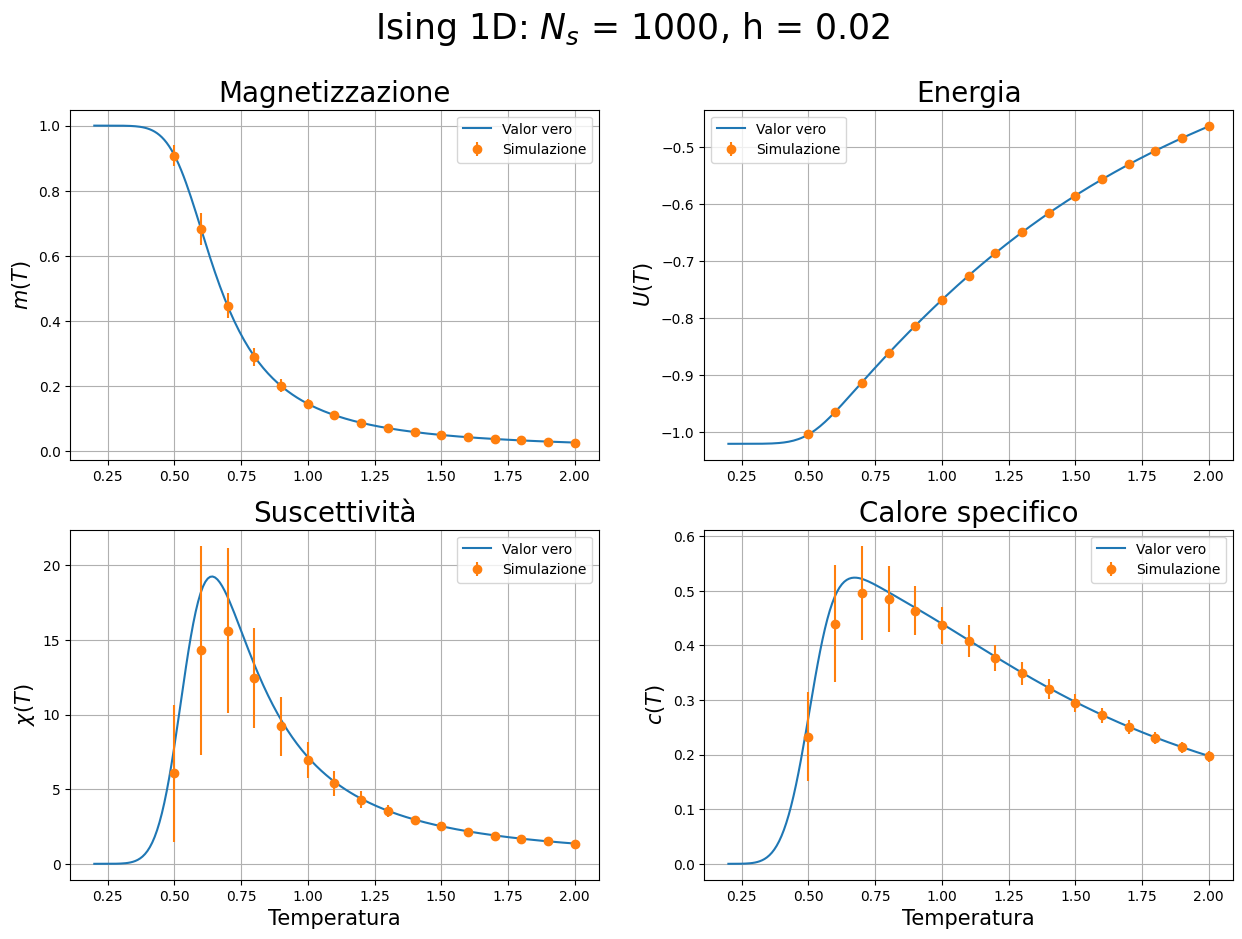
\includegraphics[page=1, width=\textwidth]{Immagini/simIsing1D/obs/obs_1000_0.02.png}
    \caption{Osservabili di un modello di Ising 1D: $N_s$ = 1000, h = 0.02.}
\end{figure}

\vspace*{\fill}

\newpage

\vspace*{\fill}

\begin{figure}[htbp]
    \centering
    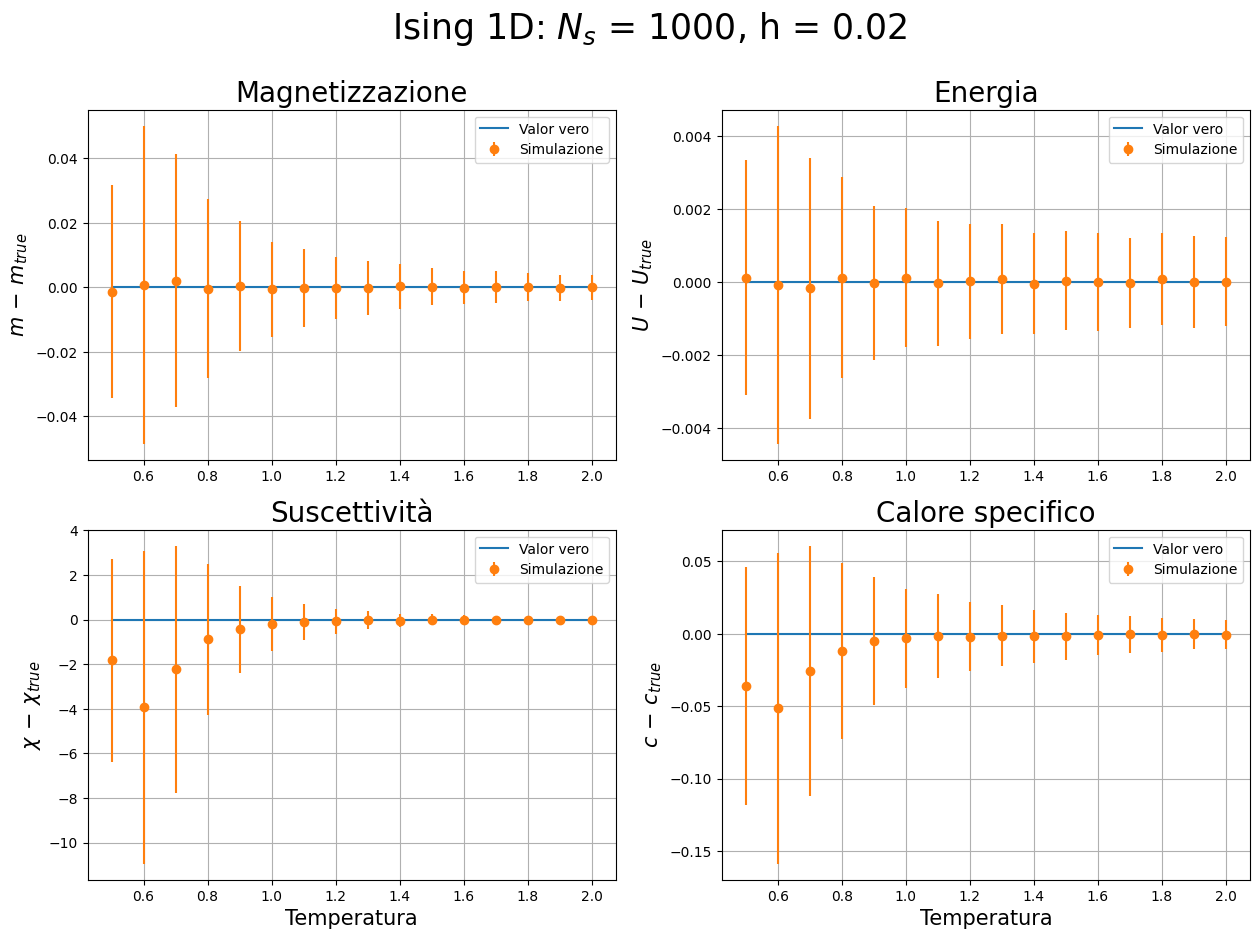
\includegraphics[page=1, width=\textwidth]{Immagini/simIsing1D/obs/obs_1000_0.02_diff.png}
    \caption{Differenza dal valor vero per un modello di Ising 1D: $N_s$ = 1000, h = 0.02.}
\end{figure}

\vspace*{\fill}

\newpage

\vspace*{\fill}

\begin{figure}[htbp]
    \centering
    \includegraphics[page=1, width=\textwidth]{Immagini/simIsing1D/obs/obs_3000_0.02.png}
    \caption{Osservabili di un modello di Ising 1D: $N_s$ = 3000, h = 0.02.}
\end{figure}

\vspace*{\fill}

\newpage

\vspace*{\fill}

\begin{figure}[htbp]
    \centering
    \includegraphics[page=1, width=\textwidth]{Immagini/simIsing1D/obs/obs_3000_0.02_diff.png}
    \caption{Differenza dal valor vero per un modello di Ising 1D: $N_s$ = 3000, h = 0.02.}
\end{figure}

\vspace*{\fill}

\newpage

\vspace*{\fill}

\begin{figure}[htbp]
    \centering
    \includegraphics[page=1, width=\textwidth]{Immagini/simIsing1D/obs/obs_6000_0.02.png}
    \caption{Osservabili di un modello di Ising 1D: $N_s$ = 6000, h = 0.02.}
\end{figure}

\vspace*{\fill}

\newpage

\vspace*{\fill}

\begin{figure}[htbp]
    \centering
    \includegraphics[page=1, width=\textwidth]{Immagini/simIsing1D/obs/obs_6000_0.02_diff.png}
    \caption{Differenza dal valor vero per un modello di Ising 1D: $N_s$ = 6000, h = 0.02.}
\end{figure}

\vspace*{\fill}

\newpage

\vspace*{\fill}

\begin{figure}[htbp]
    \centering
    \includegraphics[page=1, width=\textwidth]{Immagini/simIsing1D/obs/obs_10000_0.02.png}
    \caption{Osservabili di un modello di Ising 1D: $N_s$ = 10000, h = 0.02.}
\end{figure}

\vspace*{\fill}

\newpage

\vspace*{\fill}

\begin{figure}[htbp]
    \centering
    \includegraphics[page=1, width=\textwidth]{Immagini/simIsing1D/obs/obs_10000_0.02_diff.png}
    \caption{Differenza dal valor vero per un modello di Ising 1D: $N_s$ = 10000, h = 0.02.}
\end{figure}

\vspace*{\fill}

\newpage